% this file is encoded in utf-8
% v1.7

\documentclass[13pt, a4paper]{ntust_report} 

\usepackage{fontspec}   %加這個就可以設定字體 
\usepackage{xeCJK}       %讓中英文字體分開設置 
\setmainfont[Mapping=tex-text]{Times New Roman}            %設定主要字型,也就是英文字型 
\setCJKmainfont[AutoFakeBold=3.5]{標楷體}     %設定中文字型 
\XeTeXlinebreaklocale "zh"                %這兩行一定要加,中文才能自動換行 
\XeTeXlinebreakskip = 0pt plus 1pt       %這兩行一定要加,中文才能自動換行

\usepackage{color}

\usepackage{hyperref}
\usepackage{nameref}
\usepackage{multicol}
\usepackage{caption} 
\captionsetup[table]{skip=5pt}

%abs
\usepackage{mathtools}

\DeclarePairedDelimiter\abs{\lvert}{\rvert}%
\DeclarePairedDelimiter\norm{\lVert}{\rVert}%

% Swap the definition of \abs* and \norm*, so that \abs
% and \norm resizes the size of the brackets, and the 
% starred version does not.
\makeatletter
\let\oldabs\abs
\def\abs{\@ifstar{\oldabs}{\oldabs*}}
%
\let\oldnorm\norm
\def\norm{\@ifstar{\oldnorm}{\oldnorm*}}
\makeatother


\usepackage{setspace}
\usepackage{appendix}
\usepackage{amsmath}
\usepackage{pdfpages}




% 除非校方修改了論文格式 (margins, header, footer, 浮水印)
% 或者需要增加所用的 LaTeX 套件,
% 或者要改預設中文字型、編碼
% 否則毋須修改本檔內容
% 論文撰寫,請修改以 my_  開頭檔名的各檔案



\usepackage{titletoc}
\usepackage[nospace]{cite}  % for smart citation
\usepackage{geometry}  % for easy margin settings
\usepackage{subfigure}  % for subfigure
\usepackage{multirow}
%\usepackage[dvipdfm]{graphicx}  % for graphic   using eps
\usepackage{graphicx}  % for graphic   using eps

%\usepackage{epstopdf} % 當使用pdflatex時打開,如使用latex則不需開啟,此功能為將xxx.eps 自動判讀為XXX.pdf

%\usepackage{subfig} 
\usepackage{algorithmic}  %演算法使用
\usepackage{algorithm}

%
% margins setting
\geometry{verbose,a4paper,tmargin=3.5cm,bmargin=2cm,lmargin=3cm,rmargin=3cm}
%
\usepackage{amsmath} % 各式 AMS 數學功能
\usepackage{amssymb} % 各式 AMS 數學符號
\usepackage{mathrsfs} %草寫體數學符號,在數學模式裡用 \mathscr{E} 得草寫 E
\usepackage{listings} % 程式列表套件
%
% listing setting
\lstset{breaklines=true,% 過長的程式行可斷行
extendedchars=false,% 中文處理不需要 extendedchars
texcl=true,% 中文註解需要有 TeX 處理過的 comment line, 所以設成 true
comment=[l]\%\%,% 以雙「百分號」做為程式中文註解的起頭標記,配合 MATLAB
basicstyle=\small,% 小號字體, 約 10 pt 大小
commentstyle=\upshape,% 預設是斜體字,會影響註解裏的英文,改用正體
%language=Octave % 會將一些 octave 指令以粗體顯示
}

\usepackage{url} % 在文稿中引用網址,可以用 \url{http://www.ntust.edu.tw} 方式

% 插圖套件 graphicx
% 使用者工作流程是用 pdftex 還是 latex + dvipdfmx?
% 視情況而有不同的參數
% 這裡作自動判斷
% 參考自
% http://www.tex.ac.uk/cgi-bin/texfaq2html?label=ifpdf
%\newcommand\mydvipdfmxflow{dvipdfmx}
%\newcommand\mypdftexflow{pdftex}
%
%\ifx\pdfoutput\undefined
%  % not running pdftex
%  \usepackage[dvipdfm]{graphicx}
%  \newcommand\myworkflow{dvipdfmx}  % set the flag for hyperref
%\else
%  \ifx\pdfoutput\relax
%    % not running pdftex
%    \usepackage[dvipdfm]{graphicx}
%    \newcommand\myworkflow{dvipdfmx}  % set the flag
%  \else
%    % running pdftex, with...
%    \ifnum\pdfoutput>0
%      % ... PDF output
%      \usepackage[pdftex]{graphicx}
%      \newcommand\myworkflow{pdftex}  % set the flag
%    \else
%      %...DVI output
%      \usepackage[dvipdfm]{graphicx}
%      \newcommand\myworkflow{dvipdfmx}  % set the flag
%    \fi
%  \fi
%\fi

\usepackage{fancyhdr}  % 借用增強功能型 header 套件來擺放浮水印 
% (佔用了 central header)
% 不需要浮水印的使用者仍可利用此套件,產生所需的 header, footer
%
% 啟動 fancy header/footer 套件
\pagestyle{fancy}
\fancyhead{}  % reset left, central, right header to empty
\fancyfoot[C]{\thepage} %中間 footer 擺放頁碼
\renewcommand{\headrulewidth}{0pt} % header 的直線; 0pt 則無線

% 如果不需要任何浮水印,則請把下列介於 >>> 與 <<< 之間
% 的文字行關掉 (行首加上百分號)
%% 浮水印 >>> 
%7/23
%
% this file is encoded in utf-8
% v1.7
% 如果浮水印不是全篇需要,請把下列介於 >>> 與 <<<
% 的「全篇浮水印專用碼」關掉 (行首加百分號)
% 參考自 Keith Reckdahl 寫的 "Using Imported Graphics in LATEX2e" (epslatex.pdf) p.39
% 如果只有特定頁需要浮水印
% 則依該頁屬性使用下列之一的命令 
% 普通頁命令 \thispagestyle{WaterMarkPage}
% plain 頁命令 \thispagestyle{PlainWaterMarkPage}
% empty 頁命令 \thispagestyle{EmptyWaterMarkPage}


% 將重複使用的浮水印章
% 圖檔是 my_watermark.xxx
% 副檔名可以不加,可以是 latex 系統能處裡的任何格式:pdf, gif, png, jpg, eps, ...
% 某些圖檔格式在某些工作流程可能需要作前置處裡。
% 例如,pdflatex 無法直接處理 eps 檔
%  latex + dvipdfmx 無法直接處理 pdf, gif, png, jpg, 需要用 ebb 小工具程式
%  對圖檔產生 .bb 對應檔。
% old code
%\newsavebox{\mywatermark}
%\sbox{\mywatermark}{\includegraphics[keepaspectratio,%
%height=0.8\textheight,%
%width=0.8\textwidth]{my_watermark}}
% new code
\newsavebox{\mywatermark}
%7/23
\sbox{\mywatermark}{
\includegraphics[keepaspectratio,
width=2.5cm]{watermark/ntust_watermark.eps}}


% 將 central header 擺放浮水印的巨集指令
\newcommand{\PlaceWaterMark}{\fancyhead[C]{\setlength{\unitlength}{1in}%
\begin{picture}(0,0)%
%\put(-2.2,-6){\usebox{\mywatermark}}% old code
\put(-0.5,-5.3){\usebox{\mywatermark}}% new code
\end{picture}}%
}

\fancyhead{}  % reset left, central, right header to empty
%% 如果不需整篇論文都要浮水印
%% 則下面  >>> 與 <<< 之間的程式碼請關閉
%% >>> 全篇浮水印

\PlaceWaterMark  % 每一頁都有浮水印 (除了 plain、empty 頁以外)

% 重新定義 plain 頁面
% 每張 plain 頁面 (每一章的第一頁) 也加浮水印

\fancypagestyle{plain}{%
\fancyhead{}%
\PlaceWaterMark%
\fancyfoot{}%
\fancyfoot[C]{\thepage}
\renewcommand{\headrulewidth}{0pt}%
\renewcommand{\footrulewidth}{0pt}%
}
%% <<< 全篇浮水印

%% 如果只有一、兩頁需要有浮水印
%% 可以在該頁 (有頁碼) 使用 \thispagestyle{WaterMarkPage}
%% 此命令不影響原有的 header、footer
\fancypagestyle{WaterMarkPage}{%
\PlaceWaterMark%
}

%% 如果只有一、兩頁 plain 頁需要有浮水印 (如 摘要、自傳等)
%% 可以在該頁 (有頁碼) 使用 \thispagestyle{PlainWaterMarkPage}
%% 只有頁碼與浮水印,沒有其他的 header、footer
%% 等同於 plain page style + water mark
\fancypagestyle{PlainWaterMarkPage}{%
\fancyhead{}%
\PlaceWaterMark%
\fancyfoot{}%
\fancyfoot[C]{\thepage}
\renewcommand{\headrulewidth}{0pt}%
\renewcommand{\footrulewidth}{0pt}%
}

%% 如果只有一、兩頁 empty 頁需要有浮水印 (如封面、書名頁)
%% 可以在該頁 (無頁碼) 使用 \thispagestyle{EmptyWaterMarkPage}
%% 等同於 empty page style + water mark
\fancypagestyle{EmptyWaterMarkPage}{%
\fancyhead{}%
\PlaceWaterMark%
\fancyfoot{}%
\renewcommand{\headrulewidth}{0pt}%
\renewcommand{\footrulewidth}{0pt}%
}

\fancypagestyle{AppendixPage}{%
\fancyhead{}%
\fancyfoot{}%
\fancyfoot[C]{\thepage}
\renewcommand{\headrulewidth}{0pt}%
\renewcommand{\footrulewidth}{0pt}%
}
%% <<< 浮水印



% global page layout
\newcommand{\mybaselinestretch}{1.5}  %行距 1.5 倍 + 20%, (約為 double space)
\renewcommand{\baselinestretch}{\mybaselinestretch}  % 論文行距預設值
\parskip=2ex  % 段落之間的間隔為兩個 x 的高度
\parindent = 24Pt  % 段首內縮由 CJK 控制,所以這裡就設成不內縮

%%%%%%%%%%%%%%%%%%%%%%%%%%%%%
%  end of preamble
%%%%%%%%%%%%%%%%%%%%%%%%%%%%%  %基本的環境設定  無需改變  

\newcommand{\specialcell}[2][c]{%
  \begin{tabular}[#1]{@{}c@{}}#2\end{tabular}}

\begin{document}

	% 下列中文名詞的定義,如果以註解方式關閉取消,
% 則會以系統原先的預設值 (英文) 替代
% 名詞 \prechaptername 預設值為 Chapter
% 名詞 \postchaptername 預設值為空字串
% 名詞 \tablename 預設值為 Table
% 名詞 \figurename 預設值為 Figure

\renewcommand\prechaptername{第} % 出現在每一章的開頭的「第 x 章」
\renewcommand\postchaptername{章}
\renewcommand{\tablename}{表} % 在文章中 table caption 會以「表 x」表示
\renewcommand{\figurename}{圖} % 在文章中 figure caption 會以「圖 x」表示

% 下列中文名詞的定義,用於論文固定的各部分之命名 (出現於目錄與該頁標題)
\newcommand{\nameInnerCover}{教授推薦書}
\newcommand{\nameCommitteeForm}{論文口試委員審定書}
\newcommand{\nameCopyrightForm}{授權書}
\newcommand{\nameCabstract}{論文摘要}
\newcommand{\nameEabstract}{Abstract}
\newcommand{\nameAckn}{誌謝}
\newcommand{\nameToc}{目錄}
\newcommand{\nameLot}{表目錄}
\newcommand{\nameTof}{圖目錄}
\newcommand{\nameToa}{演算法目錄}
\newcommand{\nameSlist}{符號說明}
\newcommand{\nameRef}{參考文獻}
\newcommand{\nameVita}{自傳}
 %在此檔案處定義文章中的中文名詞

	%----------------------------------------------------------------------------------------------------------------------------------------------------------
	%%% 以下是載入前頁、本文、後頁
	% 此行請勿更動

	%----------------------------------------------------------------------------------------------------------------------------------------------------------
	% front matter 前頁
	% 包括封面、書名頁、中文摘要、英文摘要、誌謝、目錄、表目錄、圖目錄、符號說明
	% 在撰寫各章草稿時,可以把此部份「關掉」,以節省無謂的編譯時間。
	% 實際內容由
	%    my_names.tex, my_cabstract.tex, my_eabstract.tex, my_ackn.tex, my_symbols.tex
	% 決定
	% ntust_frontpages.tex 此檔只提供整體架構的定義,不需更動
	% 在撰寫各章草稿時,可以把此部份「關掉」,以節省無謂的編譯時間。
	
	%
% this file is encoded in utf-8
% v1.7
% do not change the content of this file
% unless the thesis layout rule is changed
% 無須修改本檔內容,除非校方修改了
% 封面、書名頁、中文摘要、英文摘要、誌謝、目錄、表目錄、圖目錄、符號說明
% 等頁之格式
% this file is encoded in utf-8
%v1.7

% make the line spacing in effect
\renewcommand{\baselinestretch}{\mybaselinestretch}
\large % it needs a font size changing command to be effective

% default variables definitions
% 注意!!此處只是預設值,不需更改此處
% 請更改 my_names.tex 內容
\newcommand\cTitle{論文題目}
\newcommand\eTitle{MY THESIS TITLE}
\newcommand\myCname{王鐵雄}
\newcommand\myEname{Aron Wang}
\newcommand\myStudentID{M9315048}
\newcommand\advisorCnameA{南宮明博士}
\newcommand\advisorEnameA{Dr.~Ming Nangong}
\newcommand\advisorCnameB{李斯坦博士}
\newcommand\advisorEnameB{Dr.~Stein Lee}
\newcommand\advisorCnameC{徐 石博士}
\newcommand\advisorEnameC{Dr.~Sean~Hsu}
\newcommand\univCname{國立台灣科技大學}
\newcommand\univEname{National Taiwan University of science and technology}
\newcommand\deptCname{光電工程研究所}
\newcommand\fulldeptEname{Graduate School of Electro-Optical Engineering}
\newcommand\deptEname{Electro-optical Engineering}
\newcommand\collEname{College of Engineering}
\newcommand\degreeCname{碩士}
\newcommand\degreeEname{Master of Science}
\newcommand\cYear{九十四}
\newcommand\cMonth{六}
\newcommand\cDay{十}
%\newcounter{eYear}
\newcommand\eYear{2006}
\newcommand\eMonth{June}
\newcommand\ePlace{Chungli, Taoyuan, Taiwan}


 % user's names; to replace those default variable definitions
%
% this file is encoded in utf-8
% v1.7
% 填入你的論文題目、姓名等資料
% 如果題目內有必須以數學模式表示的符號,請用 \mbox{} 包住數學模式,如下範例
% 如果中文名字是單名,與姓氏之間建議以全形空白填入,如下範例
% 英文名字中的稱謂,如 Prof. 以及 Dr.,其句點之後請以不斷行空白~代替一般空白,如下範例
% 如果你的指導教授沒有如預設的三位這麼多,則請把相對應的多餘教授的中文、英文名
%    的定義以空的大括號表示
%    如,\renewcommand\advisorCnameB{}
%          \renewcommand\advisorEnameB{}
%          \renewcommand\advisorCnameC{}
%          \renewcommand\advisorEnameC{}

% 論文題目 (中文)
\renewcommand\cTitle{%我的碩士論文題目 
校舍耐震資料庫之資料探勘
}

% 論文題目 (英文)
\renewcommand\eTitle{%My Thesis Title  
Data Mining on Aseismic School Building Database 
%My Thesis Title  \mbox{$\cal{H}_\infty$} and \mbox{Al$_x$Ga$_{1-x}$As}
}

% 我的姓名 (中文)
\renewcommand\myCname{高偉格}

% 我的姓名 (英文)
\renewcommand\myEname{Kao, Wei-Ko}

%我的學號
\renewcommand\myStudentID{D9505501}

% 指導教授A的姓名 (中文)
\renewcommand\advisorCnameA{陳鴻銘 博士}

% 指導教授A的姓名 (英文)
\renewcommand\advisorEnameA{Dr. Hung-Ming Cheng}

% 指導教授B的姓名 (中文)
\renewcommand\advisorCnameB{}

% 指導教授B的姓名 (英文)
\renewcommand\advisorEnameB{}

% 指導教授C的姓名 (中文)
\renewcommand\advisorCnameC{}

% 指導教授C的姓名 (英文)
\renewcommand\advisorEnameC{}

% 校名 (中文)
\renewcommand\univCname{國立台灣科技大學}

% 校名 (英文)
%\renewcommand\univEname{National Taiwan University of science and technology}

% 系所名 (中文)
\renewcommand\deptCname{營~建~工~程~系}

% 系所全名 (英文)
%\renewcommand\fulldeptEname{Graduate School of Electro-Optical Engineering}

% 系所短名 (英文, 用於書名頁學位名領域)
%\renewcommand\deptEname{Electro-Optical Engineering}

% 學院英文名 (如無,則以空的大括號表示)
%\renewcommand\collEname{College of Electrical and Communication Engineering}

% 學位名 (中文)
\renewcommand\degreeCname{博士學位}

% 學位名 (英文)
%\renewcommand\degreeEname{Master of Science}

% 口試年份 (中文、民國)
\renewcommand\cYear{一零二}

% 口試月份 (中文)
\renewcommand\cMonth{七} 

% 口試月份 (中文)
\renewcommand\cDay{七} 

% 口試年份 (阿拉伯數字、西元)
%\renewcommand\eYear{2009} 

% 口試月份 (英文)
%\renewcommand\eMonth{July}

% 學校所在地 (英文)
%\renewcommand\ePlace{Taipei, Taiwan}

%畢業級別;用於書背列印;若無此需要可忽略
\newcommand\GraduationClass{95}

%%%%%%%%%%%%%%%%%%%%%%
\newcommand\itsempty{}
%%%%%%%%%%%%%%%%%%%%%%%%%%%%%%%
%       ntust cover 封面
%%%%%%%%%%%%%%%%%%%%%%%%%%%%%%%
%
\begin{titlepage}
% no page number
% next page will be page 1

% aligned to the center of the page
\begin{center}
% font size (relative to 12 pt):
% \large (14pt) < \Large (18pt) < \LARGE (20pt) < \huge (24pt)< \Huge (24 pt)
%



\begin{figure}[htbp]
	\begin{minipage}[t]{5cm} 
		\raggedright
		
\includegraphics[width=1.1in]{frontpages/ntust_logo.eps}
		\label{fig:ntust_logo}
		\vspace{0.5cm}
	\end{minipage}% 
	\begin{minipage}[b]{0.5\textwidth} 
	\centering
	\makebox[3cm][c]{\Huge{\univCname}}\\  %顯示中文校名
	\vspace{0.5cm}
	\makebox[3cm][c]{\Huge{\deptCname}}\\ %顯示中文系所名
	\vspace{0.5cm}
	\makebox[3cm][c]{\Huge{\degreeCname 論文}}\\ %顯示論文種類 (中文)
	\vspace{0.5cm}
	\end{minipage}%
\\ 
\rule{16cm}{3pt}
\end{figure}
%\hfill


%\makebox[8cm][s]{\textbf{\Huge{\degreeCname 論文(初稿)}}}\\ %顯示論文種類 (中文)
\vspace{1cm}
%
% Set the line spacing to single for the titles (to compress the lines)
\renewcommand{\baselinestretch}{1}   %行距 1 倍
%\large % it needs a font size changing command to be effective
\textbf{\LARGE{\cTitle}}\\  % 中文題目
%
\vspace{1cm}
%
\Large{\eTitle}\\ %英文題目
\vspace{5cm}
% \makebox is a text box with specified width;
% option s: stretch
% use \makebox to make sure
% 「研究生:」 與「指導教授:」occupy the same width
\hspace{4.5cm} \makebox[3cm][s]{\Large{研 究 生:}}
\Large{\myCname}  % 顯示作者中文名
\hfill \makebox[1cm][s]{}\\
%
\vspace{0.3cm}
\hspace{4.5cm} \makebox[3cm][s]{\Large{學號:}}
\Large{\myStudentID}  %顯示指導教授A中文名
\hfill \makebox[1cm][s]{}\\
%
\vspace{1cm}
\hspace{4.5cm} \makebox[3cm][s]{\Large{指導教授:}}
\Large{\advisorCnameA}  %顯示指導教授A中文名
\hfill \makebox[1cm][s]{}\\
%
% 判斷是否有共同指導的教授 B
\ifx \advisorCnameB  \itsempty
\relax % 沒有 B 教授,所以不佔版面,不印任何空白
\else
% 共同指導的教授 B
\hspace{4.5cm} \makebox[3cm][s]{}
\Large{\advisorCnameB}  %顯示指導教授B中文名
\hfill \makebox[1cm][s]{}\\
\fi
%
% 判斷是否有共同指導的教授 C
\ifx \advisorCnameC  \itsempty
\relax % 沒有 C 教授,所以不佔版面,不印任何空白
\else
% 共同指導的教授 C
\hspace{4.5cm} \makebox[3cm][s]{}
\Large{\advisorCnameC}  %顯示指導教授C中文名
\hfill \makebox[1cm][s]{}\\
\fi
%
\vfill
\makebox[10cm][s]{\Large{中華民國\cYear 年\cMonth 月\cDay 日}}%
%
\end{center}
% Resume the line spacing to the desired setting
\renewcommand{\baselinestretch}{\mybaselinestretch}   %恢復原設定
% it needs a font size changing command to be effective
% restore the font size to normal
\normalsize
\end{titlepage}
%%%%%%%%%%%%%%

%% 從摘要到本文之前的部份以小寫羅馬數字印頁碼
% 但是從「書名頁」(但不印頁碼) 就開始計算
%\setcounter{page}{1}
\pagenumbering{Roman}
%\pagenumbering{arabic}
%%%%%%%%%%%%%%%%%%%%%%%%%%%%%%%
%       指導教授推薦書 
%%%%%%%%%%%%%%%%%%%%%%%%%%%%%%%
%
% insert the printed standard form when the thesis is ready to bind
% 在口試完成後,再將已簽名的推薦書放入以便裝訂
% create an entry in table of contents for 推薦書
% 目前送出空白頁
%\newpage{\thispagestyle{empty}\addcontentsline{toc}{chapter}{\nameInnerCover}\mbox{}\clearpage}%
%\newpage

% 判斷是否要浮水印?
\ifx\mywatermark\undefined 
  \thispagestyle{empty}  % 無頁碼、無 header (無浮水印)
\else
  \thispagestyle{EmptyWaterMarkPage} % 無頁碼、有浮水印
\fi

%%%%%%%%%%%%%%%%%%%%%%%%%%%%%%%%%%%%%%%%%%%%%%%%%%%%%%%%%%%%%%%
%%no page number
%% create an entry in table of contents for 書名頁
%\addcontentsline{toc}{chapter}{\nameInnerCover}
%
%
%% aligned to the center of the page
%\begin{center}
%% font size (relative to 12 pt):
%% \large (14pt) < \Large (18pt) < \LARGE (20pt) < \huge (24pt)< \Huge (24 pt)
%% Set the line spacing to single for the titles (to compress the lines)
%\renewcommand{\baselinestretch}{1}   %行距 1 倍
%% it needs a font size changing command to be effective
%%中文題目
%\Large{\cTitle}\\ %%%%%
%\vspace{1cm}
%% 英文題目
%\Large{\eTitle}\\ %%%%%
%%\vspace{1cm}
%\vfill
%% \makebox is a text box with specified width;
%% option s: stretch
%% use \makebox to make sure
%% 「研究生:」 與「指導教授:」occupy the same width
%\makebox[3cm][s]{\large{研 究 生:}}
%\makebox[3cm][l]{\large{\myCname}} %%%%%
%\hfill
%\makebox[2cm][s]{\large{Student: }}
%\makebox[5cm][l]{\large{\myEname}}\\ %%%%%
%%
%%\vspace{1cm}
%%
%\makebox[3cm][s]{\large{指導教授:}}
%\makebox[3cm][l]{\large{\advisorCnameA}} %%%%%
%\hfill
%\makebox[2cm][s]{\large{Advisor: }}
%\makebox[5cm][l]{\large{\advisorEnameA}}\\ %%%%%
%%
%% 判斷是否有共同指導的教授 B
%\ifx \advisorCnameB  \itsempty
%\relax % 沒有 B 教授,所以不佔版面,不印任何空白
%\else
%%共同指導的教授B
%\makebox[3cm][s]{}
%\makebox[3cm][l]{\large{\advisorCnameB}} %%%%%
%\hfill
%\makebox[2cm][s]{}
%\makebox[5cm][l]{\large{\advisorEnameB}}\\ %%%%%
%\fi
%%
%% 判斷是否有共同指導的教授 C
%\ifx \advisorCnameC  \itsempty
%\relax % 沒有 C 教授,所以不佔版面,不印任何空白
%\else
%%共同指導的教授C
%\makebox[3cm][s]{}
%\makebox[3cm][l]{\large{\advisorCnameC}} %%%%%
%\hfill
%\makebox[2cm][s]{}
%\makebox[5cm][l]{\large{\advisorEnameC}}\\ %%%%%
%\fi
%%
%% Resume the line spacing to the desired setting
%\renewcommand{\baselinestretch}{\mybaselinestretch}   %恢復原設定
%\large %it needs a font size changing command to be effective
%%
%\vfill
%\makebox[4cm][s]{\large{\univCname}}\\% 校名
%\makebox[6cm][s]{\large{\deptCname}}\\% 系所名
%\makebox[3cm][s]{\large{\degreeCname 論文}}\\% 學位名
%%
%%\vspace{1cm}
%\vfill
%\large{A Thesis}\\%
%\large{Submitted to }%
%%
%\large{\fulldeptEname}\\%系所全名 (英文)
%%
%%
%\ifx \collEname  \itsempty
%\relax % 沒有學院名 (英文),所以不佔版面,不印任何空白
%\else
%% 有學院名 (英文)
%\large{\collEname}\\% 學院名 (英文)
%\fi
%%
%\large{\univEname}\\%校名 (英文)
%%
%\large{in Partial Fulfillment of the Requirements}\\
%%
%\large{for the Degree of}\\
%%
%\large{\degreeEname}\\%學位名(英文)
%
%\large{in}\\
%%
%\large{\deptEname}\\%系所短名(英文;表明學位領域)
%%
%\large{\eMonth\ \eYear}\\%月、年 (英文)
%%
%\large{\ePlace}% 學校所在地 (英文)
%\vfill
%\large{中華民國}%
%\large{\cYear}% %%%%%
%\large{年}%
%\large{\cMonth}% %%%%%
%\large{月}\\
%\end{center}
%% restore the font size to normal
%\normalsize
%\clearpage


%%%%%%%%%%%%%%%%%%%%%%%%%%%%%%%%%%%%%%%%%%%%%%%%%%%%%%%%%%%%%%%%%%%%%
%%%%%%%%%%%%%%%%%%%%%%%%%%%%%%%
%       論文口試委員審定書 (計頁碼,但不印頁碼) 
%%%%%%%%%%%%%%%%%%%%%%%%%%%%%%%
%
% insert the printed standard form when the thesis is ready to bind
% 在口試完成後,再將已簽名的審定書放入以便裝訂
% create an entry in table of contents for 審定書
% 目前送出空白頁

%\newpage{\thispagestyle{empty}\addcontentsline{toc}{chapter}{\nameCommitteeForm}\mbox{}\clearpage}%


%%%%%%%%%%%%%%%%%%%%%%%%%%%%%%%
%       中文摘要 
%%%%%%%%%%%%%%%%%%%%%%%%%%%%%%%
%
\newpage
\thispagestyle{plain}  % 無 header,但在浮水印模式下會有浮水印
% create an entry in table of contents for 中文摘要
\addcontentsline{toc}{chapter}{\nameCabstract}

% aligned to the center of the page
\begin{center}
% font size (relative to 12 pt):
% \large (14pt) < \Large (18pt) < \LARGE (20pt) < \huge (24pt)< \Huge (24 pt)
% Set the line spacing to single for the names (to compress the lines)
\renewcommand{\baselinestretch}{1}   %行距 1 倍
% it needs a font size changing command to be effective
%\large{\cTitle}\\  %中文題目
%\vspace{0.83cm}
% \makebox is a text box with specified width;
% option s: stretch
% use \makebox to make sure
% each text field occupies the same width
%\makebox[1.5cm][s]{\large{學生:}}
%\makebox[3cm][l]{\large{\myCname}} %學生中文姓名
%\hfill
%
%\makebox[3cm][s]{\large{指導教授:}}
%\makebox[3cm][l]{\large{\advisorCnameA}} \\ %教授A中文姓名
%
% 判斷是否有共同指導的教授 B
\ifx \advisorCnameB  \itsempty
\relax % 沒有 B 教授,所以不佔版面,不印任何空白
\else
%共同指導的教授B
\makebox[1.5cm][s]{}
\makebox[3cm][l]{} %%%%%
\hfill
\makebox[3cm][s]{}
\makebox[3cm][l]{\large{\advisorCnameB}}\\ %教授B中文姓名
\fi
%
% 判斷是否有共同指導的教授 C
\ifx \advisorCnameC  \itsempty
\relax % 沒有 C 教授,所以不佔版面,不印任何空白
\else
%共同指導的教授C
\makebox[1.5cm][s]{}
\makebox[3cm][l]{} %%%%%
\hfill
\makebox[3cm][s]{}
\makebox[3cm][l]{\large{\advisorCnameC}}\\ %教授C中文姓名
\fi
%
%\vspace{0.42cm} %2013/06/06
\vspace{0.38cm}
%
%\large{\univCname}\large{\deptCname}\\ %校名系所名
%\vspace{0.83cm}
%\vfill
\makebox[2.5cm][s]{\LARGE{中文摘要}}\\
\end{center}
% Resume the line spacing to the desired setting
\renewcommand{\baselinestretch}{\mybaselinestretch}   %恢復原設定
%it needs a font size changing command to be effective
% restore the font size to normal
\normalsize
%%%%%%%%%%%%%

台灣國家實驗研究院地震工程研究中心(NCREE)在九二一大地震後,與教育部合作執行加速國中小老舊校舍及相關設備補強整建計畫,評估全台灣的各級學校校舍之耐震能力,在此計畫執行的過程中產生了大量的評估與調查資料,因此 NCREE 便建立了一個校舍耐震能力資料庫來收集各種相關的資料,收集了包括校舍的各種設計參數、材料強度、校舍現況及年齡、技師的評估與補強建議方案、實際補強的金額與補強方法等。此一資料庫所收集的校舍資料數量龐大,除了當初設計的目的之外,應該還潛藏難以由人直接判斷取得的知識(knowledge)、模式(pattern),而資料探勘(Data Mining)就是用來分析這種數量龐大的資料,可以從中找出潛藏知識的相關技術的統稱,本研究之目的即為利用資料探勘技術來發掘潛藏於此校舍耐震資料庫中的知識,並從資料探勘的四種主要分析方法:回歸、分類、分群、關聯出發,分別探討各種方法在此資料庫中有何可能的分析方向,有哪些可能的潛藏知識,並進行分析,最後得到了三個有用且可靠度足夠的關係模型,分別為校舍資訊與耐震能力之關係模型、校校舍資訊與破壞構件之關係模型以及校舍資訊與補強經費之關係模型。
	

%%%%%%%%%%%%%%%%%%%%%%%%%%%%%%%
%       英文摘要 
%%%%%%%%%%%%%%%%%%%%%%%%%%%%%%%
%
\newpage
\thispagestyle{plain}  % 無 header,但在浮水印模式下會有浮水印

% create an entry in table of contents for 英文摘要
\addcontentsline{toc}{chapter}{\nameEabstract}

% aligned to the center of the page
\begin{center}
% font size:
% \large (14pt) < \Large (18pt) < \LARGE (20pt) < \huge (24pt)< \Huge (24 pt)
% Set the line spacing to single for the names (to compress the lines)
\renewcommand{\baselinestretch}{1}   %行距 1 倍
%\large % it needs a font size changing command to be effective
%\large{\eTitle}\\  %英文題目
%\vspace{0.83cm}
% \makebox is a text box with specified width;
% option s: stretch
% use \makebox to make sure
% each text field occupies the same width
%\makebox[2cm][s]{\large{Student: }}
%\makebox[5cm][l]{\large{\myEname}} %學生英文姓名
%\hfill
%
%\makebox[2cm][s]{\large{Advisor: }}
%\makebox[5cm][l]{\large{\advisorEnameA}} \\ %教授A英文姓名
%
% 判斷是否有共同指導的教授 B
\ifx \advisorCnameB  \itsempty
\relax % 沒有 B 教授,所以不佔版面,不印任何空白
\else
%共同指導的教授B
\makebox[2cm][s]{}
\makebox[5cm][l]{} %%%%%
\hfill
\makebox[2cm][s]{}
\makebox[5cm][l]{\large{\advisorEnameB}}\\ %教授B英文姓名
\fi
%
% 判斷是否有共同指導的教授 C
\ifx \advisorCnameC  \itsempty
\relax % 沒有 C 教授,所以不佔版面,不印任何空白
\else
%共同指導的教授C
\makebox[2cm][s]{}
\makebox[5cm][l]{} %%%%%
\hfill
\makebox[2cm][s]{}
\makebox[5cm][l]{\large{\advisorEnameC}}\\ %教授C英文姓名
\fi
%
%\vspace{0.42cm}
%\large{Submitted to }\large{\fulldeptEname}\\  %英文系所全名
%
\ifx \collEname  \itsempty
\relax % 如果沒有學院名 (英文),則不佔版面,不印任何空白
\else
% 有學院名 (英文)
%\large{\collEname}\\% 學院名 (英文)
\fi
%
%\large{\univEname}\\  %英文校名
%\vspace{0.83cm}
%\vfill
%
\large{ABSTRACT}\\
%\vspace{0.5cm}
\end{center}
% Resume the line spacing the desired setting
\renewcommand{\baselinestretch}{\mybaselinestretch}   %恢復原設定
%\large %it needs a font size changing command to be effective
% restore the font size to normal
\normalsize
%%%%%%%%%%%%%

台灣國家實驗研究院地震工程研究中心(NCREE)在九二一大地震後,與教育部合作評估全台灣的各級學校校舍之耐震能力,在此計畫執行的過程中產生了大量的評估與調查資料,因此 NCREE 便建立了一個校舍耐震能力資料庫來收集各種相關的資料,收集了包括校舍的各種設計參數、材料強度、校舍現況及年齡、技師的評估與補強建議方案、實際補強的金額與補強方法等。收集的校舍資料數量龐大,除了當初設計的目的之外,應該還潛藏難以由人直接判斷取得的知識(knowledge)、模式(pattern)。資料探勘(Data Mining)就是用來分析這種數量龐大的資料,從中找出潛藏的知識的相關技術的統稱,本研究之目的即為利用資料探勘技術來發掘潛藏於此校舍耐震資料庫中的知識,本研究從資料探勘的四種主要分析方法:回歸、分類、分群、關聯出發,分別探討各種方法在此資料庫中有何可能的分析方向,有哪些可能的潛藏知識,並進行分析,最後得到了三個有用的預測模型,分別為校舍耐震能力預測模型、校舍破壞模式預測模型以及校舍補強經費預估模型。
	
In general, the aseismic ability of buildings is analyzed using nonlinear models. To obtain buildings’ aseismic abilities, numerical models are constructed based on the structural configuration and material properties of buildings, and their stress responses and behaviors are simulated. This method is complex, time-consuming, and should only be conducted by professionals. In the past, soft computing techniques have been applied in the construction field to predict the particular stress responses and behaviors; however, only a few studies have been made to predict specific properties of entire buildings. In this study, a Weighted Genetic Programming system is developed to construct the relation models between the aseismic capacity of school buildings, and their basic design parameters. This is based on information from the database of school buildings, as well as information regarding the aseismic capacity of school buildings analyzed using complete nonlinear methods. This system can be further applied to predict the aseismic capacity of the school buildings.

%%%%%%%%%%%%%%%%%%%%%%%%%%%%%%%
%       誌謝 
%%%%%%%%%%%%%%%%%%%%%%%%%%%%%%%
%
% Acknowledgment
\newpage
\chapter*{\protect\makebox[5cm][s]{\nameAckn}} %\makebox{} is fragile; need protect

\addcontentsline{toc}{chapter}{\nameAckn}






%%%%%%%%%%%%%%%%%%%%%%%%%%%%%%%
%       目錄 
%%%%%%%%%%%%%%%%%%%%%%%%%%%%%%%
%
% Table of contents

\newpage


\renewcommand{\contentsname}{\protect\makebox[5cm][s]{\nameToc}}
%\makebox{} is fragile; need protect
\addcontentsline{toc}{chapter}{\nameToc}
\setcounter{tocdepth}{2}
\tableofcontents




%%%%%%%%%%%%%%%%%%%%%%%%%%%%%%%
%       圖目錄 
%%%%%%%%%%%%%%%%%%%%%%%%%%%%%%%
%
% List of Figures
\newcommand{\loflabel}{圖}
\newpage
\renewcommand{\numberline}[1]{\loflabel~#1\hspace*{1em}}
\renewcommand{\listfigurename}{\protect\makebox[5cm][s]{\nameTof}}
%\makebox{} is fragile; need protect
\addcontentsline{toc}{chapter}{\nameTof}
\listoffigures

%%%%%%%%%%%%%%%%%%%%%%%%%%%%%%%
%       表目錄 
%%%%%%%%%%%%%%%%%%%%%%%%%%%%%%%
%
% List of Tables
\newcommand{\lotlabel}{表}
\newpage
\renewcommand{\numberline}[1]{\lotlabel~#1\hspace*{1em}}
\renewcommand{\listtablename}{\protect\makebox[5cm][s]{\nameLot}}
%\makebox{} is fragile; need protect
\addcontentsline{toc}{chapter}{\nameLot}
\listoftables

%%%%%%%%%%%%%%%%%%%%%%%%%%%%%%%
%       演算法目錄 
%%%%%%%%%%%%%%%%%%%%%%%%%%%%%%%
%
% List of Figures
%\newpage
%\renewcommand{\listalgorithmname}{\protect\makebox[5cm][s]{\nameToa}}
%\makebox{} is fragile; need protect
%\addcontentsline{toc}{chapter}{\nameToa}
%\listofalgorithms


%%%%%%%%%%%%%%%%%%%%%%%%%%%%%%%
%       符號說明 
%%%%%%%%%%%%%%%%%%%%%%%%%%%%%%%
%
% Symbol list
% define new environment, based on standard description environment
% adapted from p.60~64, <<The LaTeX Companion>>, 1994, ISBN 0-201-54199-8
%\newcommand{\SymEntryLabel}[1]%
% {\makebox[3cm][l]{#1}}
%
%\newenvironment{SymEntry}
%   {\begin{list}{}%
%       {\renewcommand{\makelabel}{\SymEntryLabel}%
%        \setlength{\labelwidth}{3cm}%
%        \setlength{\leftmargin}{\labelwidth}%
%        }%
%   }%
%   {\end{list}}
%%
%\newpage
%\chapter*{\protect\makebox[5cm][s]{\nameSlist}} %\makebox{} is fragile; need protect
%\addcontentsline{toc}{chapter}{\nameSlist}
%%
% this file is encoded in utf-8
% v1.7
%  各符號以 \item[] 包住,然後接著寫說明
% 如果符號是數學符號,應以數學模式表示,以取得正確的字體
% 如果符號本身帶有方括號,則此符號可以用大括號 {} 包住保護
\begin{SymEntry}

\item[$Af$]
總樓地板面積

\item[$A_C$]
校舍破壞地表加速度

\item[$A_D$]
校舍所需承受之~475~年週期最大地震之地表加速度

\item[$CDR$]
耐震需求比

\item[$C$]
訓練模型時之懲罰值(Cost)參數

\item[$\bar{C}$]
WGP~決策樹中之常數端點

\item[$C_E$]
$Is$~值轉換之~$A_C$~等意義數值

\item[$ClaAc$]
一樓教室柱總斷面積

\item[$CorAc$]
一樓走廊外柱總斷面積

\item[$D\_isR$]
校舍耐震資料庫中紀錄校舍是否需要補強之屬性

\item[$E$]
初步評估之基本耐震性能

\item[$F$]
WGP~運算樹中,代表節點之運算子方程式

\item[$f_i$]
WGP~運算樹中,第~$i$~個節點之運算子方程式

\item[$I$]
用途係數

\item[$InsAc$]
一樓隔間柱總斷面積

\item[$Is$]
初步評估之耐震指標

\item[$K$]
K-means~分群方法之初始群集數

\item[$N$]
資料總數

\item[$NF$]
校舍樓層數

\item[$NI$]
輸入參數的數量

\item[$NL$]
運算層的層數

\item[$N_g$]
需要最佳化的基因數量

\item[$O$]
偏移變數

\item[$P_i$]
WGP~運算樹中之第~$i$~個輸入屬性

\item[$P_1$]
樓層數,WGP~建立之校舍耐震能力關係模型參數之一

\item[$P_2$]
鋼筋強度,WGP~建立之校舍耐震能力關係模型參數之一

\item[$P_3$]
混凝土強度,WGP~建立之校舍耐震能力關係模型參數之一

\item[$P_4$]
校舍長度,WGP~建立之校舍耐震能力關係模型參數之一

\item[$P_5$]
校舍深度,WGP~建立之校舍耐震能力關係模型參數之一

\item[$P_6$]
教室柱數量,WGP~建立之校舍耐震能力關係模型參數之一

\item[$P_7$]
教室柱斷面積,WGP~建立之校舍耐震能力關係模型參數之一

\item[$P_8$]
是否有走廊,WGP~建立之校舍耐震能力關係模型參數之一

\item[$P_9$]
二樓樓地板面積,WGP~建立之校舍耐震能力關係模型參數之一

\item[$P_{10}$]
總樓地板面積,WGP~建立之校舍耐震能力關係模型參數之一

\item[$P_{11}$]
$S_{DS}$,校舍的震區設計水平譜加速度係數,WGP~建立之校舍耐震能力關係模型參數之一

\item[$P_{12}$]
$S_{D1}$,一秒週期的設計譜加速度,WGP~建立之校舍耐震能力關係模型參數之一

\item[$P_{13}$]
教室數量,WGP~建立之校舍耐震能力關係模型參數之一

\item[$P_{14}$]
校舍建築物的跨距,WGP~建立之校舍耐震能力關係模型參數之一

\item[$R^2$]
決定係數

\item[$S_i$]
第~$i$~個輸入參數的重要度

\item[$S_{aD}$]
一般工址或近斷層區域之工址設計水平譜加速度係數

\item[$T$]
建築物基本振動週期

\item[$T_{adj}$]
$C_E$~值修正因子

\item[$T_0^D$]
$S_{D1}/S_{DS}$

\item[$T_{AC}$]
柱等效強度

\item[$T_{AW}$]
牆等效強度

\item[$W_{ij}$]
類神經網路中第~$i$~個輸入層單元與第~$j$~個輸出層單元間之連結權重

\item[$X_i$]
所建構模型中第~$i$~個輸入屬性,也可做為類神經網路中,輸入層第~$i$~個處理單元之輸入值

\item[$Y$]
所建構模型中之輸出屬性

\item[$Y_j$]
類神經網路中輸出層第~$j$~個處理單元之推論輸出值

\item[$k$]
$k$~群交叉驗證初始時,資料的分群數量

\item[$k'$]
Random subsampling~驗證方法中,隨機取樣並建立模型的次數

\item[$net_j$]
類神經網路中輸出層第~$j$~個處理單元之集成函數

\item[$q_1$]
平面及立面對稱性,初步評估調整因子之一

\item[$q_2$]
軟弱層顯著性,初步評估調整因子之一

\item[$q_3$]
裂縫鏽蝕滲水等程度,初步評估調整因子之一

\item[$q_4$]
變形程度,初步評估調整因子之一

\item[$q_5$]
平面耐震性,初步評估調整因子之一

\item[$q_6$]
短柱嚴重性,初步評估調整因子之一

\item[$w_i$]
WGP~決策樹中,第~$i$~條分支線上之權重

\item[$x$]
輸入屬性

\item[$y$]
輸出屬性預測值

\item[$y_i$]
第~$i$~個輸出屬性預測值

\item[$\hat{y}$]
輸出屬性實際值

\item[$\hat{y_i}$]
第~$i$~個輸出屬性實際值


\item[$\alpha$]
命中率的容許誤差

\item[$\beta$]
廣義線性模型中之斜率,也就是迴歸目標

\item[$\epsilon$]
SVM~訓練模型之設定參數

\item[$\theta_j$]
類神經網路中輸出層第~$j$~個處理單元之閥值



\end{SymEntry}


\newpage
\setcounter{page}{1}
\pagenumbering{arabic}
%% 論文本體頁碼回復為阿拉伯數字計頁,並從頭起算
%\pagenumbering{arabic}
%%%%%%%%%%%%%%%%%%%%%%%%%%%%%%%% 




	%----------------------------------------------------------------------------------------------------------------------------------------------------------
	% main body 論文主體。建議以「章」為檔案分割的依據。
	% 以下為建議的命名分類
	%   introduction.tex   related_work.tex  protocol.tex  evaluation.tex  conclusion.tex
	% 做為這幾個「章」的檔案名稱,並將檔案存放於資料夾 sections/ 下
	% 實際命名方式可以隨你意
	% 在撰寫各章草稿時,可以把其他章節關掉 (行首加百分號)
	%%
% this file is encoded in utf-8
% v1.7
\chapter{\mbox{\LaTeX\ 示範}}
\label{ch:example}
這一章目的是一些基本功能的用法。最好是與原始檔案 example\_body.tex 一起對照著看。章節標題後之第一段之段首不需要內縮。

如何顯示圖檔?
圖~\ref{fig:logo} 是元智大學的校徽,以保持長寬比例,寬 2~cm,中間對齊顯示。插圖的標題須在圖的下方。如果是從別的文獻引用,出處則註記於圖標題下方。
\begin{figure}[htbp]
\centering 
\includegraphics[%
  width=2cm,keepaspectratio]{example/example_fig}
\caption{\label{fig:logo}校徽 The logo.}
(This logo comes from the school web page.)
\end{figure}

如何顯示表格?表~\ref{tb:income_2003} 是示範簡易的 $3\times3$ 的表格,除了第一欄是中間對齊以外,第二、三欄是向右對齊。表格的標題須在表格上方。或者,使用只有橫線的表格,如表~\ref{tb:income_2003_v2}。資料的出處則註記於表格下方。
%
\begin{table}[htbp]
\caption{\label{tb:income_2003}Gross income of the first two quarters of
year 2003.}
\centering \begin{tabular}{|c|r|r|}
\hline 
&
Restaurant&
Store\tabularnewline
\hline
\hline 
Q1&
\$123,000&
\$75,000\tabularnewline
\hline 
Q2&
\$45,000&
\$131,000\tabularnewline
\hline
\end{tabular}\\
(This table is made up for demonstration purpose.)
\end{table}%
%
\begin{table}[htbp]
\caption{\label{tb:income_2003_v2}Gross income of the first two quarters of
year 2003. Version 2.}
\centering \begin{tabular}{crr}
\hline 
&
Restaurant&
Store\tabularnewline
\hline
Q1&
\$123,000&
\$75,000\tabularnewline
 Q2&
\$45,000&
\$131,000\tabularnewline
\hline
\end{tabular}\\
(This table is made up for demonstration purpose.)
\end{table}


現在來示範參考文獻的引用。根據文獻\cite{ieee_dmr_2_50_2002_chou} 的說法,此實驗必須湊齊五大元素\cite{jap_093_1108_2003_kondakov, ieee_ed_50_1830_2003_oriols, Chem.Mater._8_1365_1996_Papadimitrakopoulos, jap_079_2745_1996_scott, jap_087_8049_2000_adachi, jap_089_1704_2001_brutting, jap_089_4673_2001_popovic, synth.met._132_9_2002_nomura, cjk_book, thinfilm_macleod_2001},並用天火燒之始能畢其功。


\chapter{數學式子}
我們在第 \pageref{ch:example} 頁示範了如何處理插圖以及表格。在這一章,我們來看數學公式的處理。在本文行內要書寫數學符號、式子,可以用錢符號前後包夾住表示式。如 \$ax+b=0\$ 會顯示 $ax+b=0$;如果要單獨展示數學公式,則用 \verb+\[+ 以及 \verb+\]+ 包夾住表示式。如下
\[
\sum_{k=1}^{\infty}\frac{1}{n^2}
\]

如果公式要編號碼,則要用\verb+\begin{equation}+ 以及 \verb+\end{equation}+,並在式子中加上 \verb+\label{}+ 的標籤。如
\begin{equation}
  \frac{df}{dx} \equiv \lim_{\Delta x \rightarrow 0} \frac{f(x+\Delta x) - f(x)}{\Delta x}   \label{eq:diff_def}
\end{equation}
我們可以在公式 (\ref{eq:diff_def}) 看到微分的定義。

可以參考李果正先生寫的《大家來學 {\LaTeX}》,學習更多的技巧。\\
\textless{}\url{http://edt1023.sayya.org/tex/latex123/index.html}\textgreater{}

\chapter{元智大學論文格式規範}
(本文節自《元智大學研究所學位論文格式規範條例》,文中所提之附件,\\
詳見\textless{}\url{http://www.yzu.edu.tw/admin/1/8_7.htm}\textgreater{})

\section{規格說明}
\begin{description}
\item[封面]  教務處統一格式樣本,如附件一,經教育部核可分組者是否加註組別及封面紙由各所自定。
\item[書名頁] 包括論文中英文名稱,著者及指導教授中英文姓名、校名、所名、學位論文別、提送論文英文說明及地名,提送年月等,如附件二。
\item[口試委員會審定書] 教務處統一格式樣本,如附件四,正本由各所彙整送交教務處,影本裝訂於論文內。
\item[授權書] 無論是否同意開放學術利用,本頁均須裝訂,如附件三,並與提要電子檔案開放使用欄表達一致。 (另有國科會授權書) 
\item[中英文摘要] 內容應說明研究目的,資料來源,研究方法及結果等,約 500--1000 字,並以一頁為限。須有中文摘要及英文摘要,分頁書寫,格式如附件五、六。
\item[論文尺寸及紙張] 以 $210\,\mathrm{mm} \times 297\,\mathrm{mm}$ 規格 A4 紙張繕製。封面封底採用 150 磅以上布紋紙或卡紙,顏色均由各所指定。
\item[版面規格] 紙張頂端留邊 3.5~cm,左側留邊 4~cm,右側留邊 2~cm,底端留邊 2~cm,版面底端 1~cm 處文字版面中心線處繕打頁次。
\item[文字規格] 文章主體以中文為原則,由左至右,橫式打字繕排,文句中引用之外語原文以~(~)~號附註。
\item[頁次] (1) 中文摘要至圖表目錄等,以 i, ii, iii, \ldots\ 等小寫羅馬數字連續編頁。書名頁、審定書雖無須印出頁碼,但仍應編入同此之頁碼。\\
(2) 論文中第一章以至附錄,均以 1, 2, 3, \ldots\ 等阿拉伯數字連續編頁。
\item[裝訂] 自論文本左端裝釘,書背外貼紙邊,打印畢業級別、學位論文別、論文名稱、校、院、所名、著者姓名。 (見附件十八)。
\end{description}

\section{操作細則}

\begin{description}
\item[目錄] 按本規範所訂「論文編印項目次序」各項順序,依次編排論文內各項目名稱、章、節編號、頁次等 (見附件九、九-1,請與指導教授討論擇一採用)。
\item[圖表目錄] 文內表圖,各依應用順序,不分章節連續編號,並表列一頁目次 (見附件十、十一)。
\item[符號說明] 各章節內所使用之數學及特殊符號,均集中表列一頁說明,以便參閱,表內各符號不須編號 (見附件十二)。
\item[論文本文章節編號] 章次使用一、二、⋯⋯ (或第一章、第二章⋯⋯) 等中文數字編號,節段編號則配合使用一、1-1、1-1-1、1.、 (1) 、 (或第一節、第二節、第三節、壹、一、1、(1)) 等層次順序之阿拉伯數字。
\item[論文本文章節名稱及段落層次] (見附件十三、十三-1,請與指導教授討論擇一採用)\\
(1) 章次、章名稱位於打字版面頂端中央處。\\
(2) 節次、段次均自版面左端排起,各空一、二格,繕排名稱。\\
(3) 小段以下等號次及名稱,均以行首空數格間距表明層次。
\item[論文本文行距] 中文間隔一行,每頁最少 32 行,英文間隔 1.5 或 2 行 (1.5 space or double space),每頁最少 28 行,章名下留雙倍行距。
\item[論文本文字距] 中文為密集字距,如本規範使用字距,每行最少 28 字,英文不拘。
\item[論文本文文句內數字運用] 有下列注意事項\\
(1) 描述性、非運算之簡單數字及分數數字,以中文數字表示。例:一百五十人,三萬二仟元,六十分之十七等。\\
(2) 繁長者視情況使用中文或阿拉伯數字,以簡明為宜。例:美金三十三億元 (不用 3,300,000,000 元)。\$15,349 (不用一萬五千三百四十九美元)。
\item[論文本文方程式及公式] 有下列注意事項\\
(1) 方程式及公式應縮格排列,並與正文儘區隔分開。例如:
\[ x = \frac{-b \pm \sqrt{b^2 -4ac}}{2a}. \]\\
(2) 方程式及公式不只一個時應編排序號,該序號應以圓括弧標註於最後一行的最右邊。例如:
\begin{equation}
E = mc^2.
\end{equation}\\
(3) 在正文提到相關之方程式或公式時,須表明該方程式之名稱及序號。\\
(4) 如果方程式較長需轉行時,只能在加、減、乘、除、大於、小於等運算子符號處轉行。上下式儘可能在等號「=」處對齊。例如:
\begin{equation}
\begin{split}
f(x) &= f(0) + f'(0)x + \frac{f''(0)}{2!}x^2 + \frac{f'''(0)}{3!}x^3 +\cdots \\
    &=1+\frac{1}{2}x+\left(-\frac{1}{8}\right)x^{2}+\left(\frac{1}{16}\right)x^{3}+\cdots.
\end{split}
\end{equation}\\
(5) 正文中之分數應使用 ``/'' 以區分分子與分母。例如:1/2。
\item[論文本文註腳] 有下列注意事項\\
(1) 特殊事項論點等,可使用註腳 (Footnote) 說明。\\
(2) 註腳應依順序編號,編號標於相關文右上角%
\footnote{這是 footnote 的例子。}%
以備參閱。各章內編號連續,各章之間不相接續。\\
(3) 註腳號碼及內容繕於同頁底端版面內,與正文之間加劃橫線區隔,頁面不足可延用次頁底端版面。
\item[論文本文文獻參閱] 文中所有參考之文獻,不分中英文及章節,均依參閱順序連續編號,並將參閱編號,加中括號~[~]~號標明於參閱處。文獻資料另編錄於論文本文之後。
\item[論文本文圖表編排] 有下列注意事項\\
(1) 表號及表名列於表上方,圖號及圖名置於圖下方。資料來源及說明,一律置於表圖下方。\\
(2) 圖表內文數字應予打字或以工程字書寫。
\item[參考文獻資料編排] 所有參考文獻資料,均置於論文本文之後,獨立另起一頁,按參閱編號依次編錄,頁次仍以本文接續。
\item[附錄] 凡屬大量數據、推導、註釋有關或其他冗長被參之資料、圖表,均可分別另起一頁,編為各附錄。正文中未引用之參考文獻應列出書目置於附錄之中。
\end{description}

\chapter{兩篇短文}
論文格式規範有些要在一章的第二頁之後,有些要在整頁文字的情況下,有些要在多層次分節的情況下才看得出來。所以,附上兩篇輕鬆的短文,來展示前面各章節還沒有遇到的論文規範。

\section{南橫上的捍衛戰警—閻驊}
\label{speed}
(原文作者為閻驊,見於 \textless{}\url{http://www.1001yeah.com.tw}\textgreater{})

今年舊曆新年前,我進行了兩年來的第五度環島旅行。不過這次遇上了大麻煩!因為汽車在南橫公路接近最高點的地方拋錨。這次拋錨事件讓我非常尷尬!一、我居然在一個接近三十度的險升坡上拋錨!二、汽車拋錨之處,手機居然無法播通!三、就算手機可以播通,其實也沒啥屁用!因為南橫目前是禁止大型車進入,所以拖吊車根本無法開進來救我。那時我直覺地認為應該是汽車沒電、才會拋錨!所以我就開始裝可愛、站在路旁攔車、幫我接電。但是不知道怎麼搞的!在汽車拋錨之後的半小時,南橫似乎道路封閉似的!居然沒有半台汽車經過?半小時之後,當第一台汽車映入眼簾時,就接連著出現了十幾台汽車魚貫而來,每一位駕駛員對我的反應都是一樣的:放慢車速→拉下車窗→看看我的車子→思索三秒鐘→對我搖搖頭→加速離去。整整一小時之後,才出現了第一台願意停下來、幫我忙的車子。車主熱心地把車頭倒過來、幫我接電。結果∼我的笨蛋汽車依然無法發動!我想這下子糟糕了!我可能要宣布棄車逃亡了。

\subsection{發生了什麼事?}
不過這時奇蹟出現了!接連又來了兩台汽車、自動自發地停下來、加入修車的行列中。場面此時開始熱鬧了起來,狹小的南橫公路上停了四台車、十個人一起七嘴八舌地討論了修車方案。

\subsection{修車方法}
正好這些好心人裡頭,有兩位剛從軍中退伍的修車兵。根據他們專業的眼光來看,他們一致認為火星塞應該髒掉了!於是大家用一些很「馬蓋先」的克難方式,有說又笑地把我的引擎拆開,用衛生筷子夾著衛生紙,擦拭其中的一個火星塞%
\footnote{為何會選擇那一個火星塞來修理呢?後來我才知道他們是瞎矇的!因為台南的修車廠老闆告訴我,那一個火星塞是我汽車四個火星塞之中,
唯一沒有故障的那一個!}%
,然後我的汽車就這麼神奇地發動成功了!

 當我的汽車成功發動之後,這些幫我修車的好心人們突然問了我老婆一個問題:「請問你有男友嗎?」。我那誠實的老婆指著我、回答道:「我沒有男友,但是車主是我老公!」。於是這群好心的大男生就長嘆一聲,三台好心車、八位好心人就這麼一瞬間消失無蹤。
 
\subsection{另一項考驗}
不過我的另一個考驗在汽車發動成功之後才登場。這個考驗就是:我的時速不能低於三十公里、不然就會讓我的引擎再度熄火。況且我拋錨的路段距離台南還有兩百公里。而且接下來的路段可是峰迴路轉、路面狹窄!而且單向通車的路段也是不少!這種考驗幾乎就等於是基努李維所飾演的「捍衛戰警」一樣:就是車速一慢,炸彈立即引爆。
 
所以接下來的山路,我都是馬不停蹄地向前狂奔。遇到前方有車,幾乎都是像流氓一樣地猛按喇叭、狠狠超車。如果看到前方是單向通車的路段,我都是硬踩著油門、用超過一百公里的速度火速通過。

兩個多小時之後,我就成功地飆到台南某修車廠、總計開了兩百公里、下降了兩千九百公尺、平均下山時速約九十公里。我的耳膜與心臟都非常地疼痛! (因為車速只要低於六十公里,我的笨蛋汽車就會發出一種非常 Weak 的聲響,提醒我:「主人∼主人,我又要拋錨囉!趕快跳傘逃生吧!」,讓我心力交瘁!) 

捍衛戰警的故事就講到這裡!不過在這個故事裡頭有一個小插曲,讓我感觸良多!我這些日子以來,午夜夢迴時經常會想起。前述文字不是曾經提到,當我汽車拋錨之後的一個小時內,大約有十幾台汽車經過!但是他們對我不理不睬、也不願意對我伸出援手,讓我充滿了憤慨、大嘆世風日下、人心不古。就這個問題,我當時就問了幫我修車的那幾位年輕人:「為什麼剛才那些車主如此沒有同情心,不願意停下來幫我呢?」在正常的狀況下,這些年輕人應該會回答我:「幹!他們又不認識你,他幹麼要停下來幫你接電呢?你長得比較帥嗎?」。

我邊發問、邊推敲著他們應該會回答我的答案。因為我一直覺得這些善心人士願意停下來幫我接電,應該是看到了我那美麗又可愛的老婆楚楚可憐地站在路旁揮手吧?不過這些年輕人算是有大智慧之人,他們居然回答了一個我意料之外的答案。年輕人嚼著檳榔告訴我說:「你不知道小車幫大車接電,小車除了幫不上大車的忙之外,而且自己的小車可能也會因此沒電呢!」

另外一個年輕人接著說:「並不是別人沒心肝、不願意幫你接電!而是他們看你的汽車這麼大台、親像一艘船!深怕自己的小車不但幫不上你的忙,還會陪著你一起在南橫公路上拋錨呢!」我想了一想!年輕人的邏輯應該是正確的!因為前面那十幾台棄我於不顧的汽車真的都是像 March、Festival 之類的小車,所以我開始露出「偶真的很汗顏!」的尷尬神情。

我端詳著這台讓我出糗的老爺車,我真的認為年輕人所言屬實!因為我這台老爺車,雖然只有 2000~cc,但是外型非常不流線、而且車體奇『肥』無比,似乎是根據我的『無敵肥臉』所量身訂作的!我想大部分的人瞄過我的肥車一眼,應該誤以為那是一台 3000~cc 以上的臃腫大車吧?年輕人看我如此汗顏,就開始妙語如珠了起來:「對啊!別人還以為你是開「林肯 (臃腫大車的代表作) 」呢!就怕自己停下來幫你接電,不但幫不了林肯、還淪落成為「甘乃迪 (台語:『像一隻豬』的諧音) 」。

其實我到現在,還是無法證實「小車幫大車接電,小車不但幫不上忙,而且可能還會害了自己!」的說法是否屬實?好吧!看到這幾位好心年輕人的份上,我就當這個說法為真!

這個「幫不了林肯、反而成為甘乃迪」的理論,讓我真是感觸良多!尤其是在我的慢呆餐廳即將結束之際。

記得去年九月底,當慢呆餐廳發生了可怕的「九二四慘案%
\footnote{所謂的「九二四慘案」,請見網站!}%
」之後,我的人生就隨著這樁駭人聽聞的慘案一同 Down 入了深淵。

去年的十月初,當我將這家已經公開宣布畢業、已經被人含淚歡送的慢呆餐廳重新開幕之後。我嚐到了刻骨銘心、讓我永誌難忘的苦果!因為『死而復生』的慢呆餐廳早已經被眾人 (尤其是讀者朋友) 唾棄、業績瓦解了整整七、八成、而且一直在低檔徘徊、毫無復甦的跡象。所以在 2004 年年底的那三個月,我陷入極深的憂鬱中,我靠著高劑量的抗憂鬱藥在過活。那時我總是想著:我明明是『九二四慘案』的最大受害者,但是為何我還要揹著這種「沒有誠信」的罪名、苦苦無法翻身呢?在那段時間,我知道刻意與我疏遠的人非常地多!很多慢呆熟客從此再也不願意踏入慢呆大門!我那個剛成氣候的天方 Yeah 壇,一些能言善道的勇將也紛紛繞跑、造成論壇的大失血。我是一個感覺很細微的人,我可以很清楚地察覺我的人氣、我的形象、我的誠信都已經隨著「九二四慘案」瓦解!所以去年 Q4 的我一直活在無限恐慌與無助的情境下、就像一個溺水的人在水裡浮載浮沉,急迫地揮著手求救!如果用我的南橫故事來解釋我當時的狀況,我想很多人都以為我是期待接電的臃腫大車、深怕自己的小車不但幫不上忙,還要陪著一起拋錨、而得不償失!「不幫你,或許害了你!但是幫你,卻可能害了你跟我!何苦呢?」我想這是當時很多人對我的直覺反應吧?您覺得我在責怪當初棄我而去的廣大人群嗎?錯!我真的不想責怪任何人!而且我也沒有權利責怪!因為我們就將心比心嘛!如果我看到歐尼爾 (體重重我兩倍的 NBA 巨星) 溺水,我想我也不敢伸出援手!如果我看到一台賓士 600 拋錨在南橫、期待我幫忙接電。我大概也會跟賓士車主露出一臉無奈的笑容、心裡想著:「您老師卡好啦!幫你接電,那我的肥車一定會立即拋錨在路旁!願老天保佑你,阿彌陀佛、萬福瑪麗亞、阿門!」,然後加速駛離現場。其實我們一直酷愛告訴別人:「不要管別人怎麼想!做你自己最重要!」。錯!我現在覺得這句話並不對!為何您明明活在這個世界上,您卻可以不要在乎世界上的其他人對你的看法呢?由於大家的厚愛與抬愛,或許很多人都認為我應該是一位跟小甜甜一樣、自立自強有信心、前途光明又燦爛的一號人物。或許我被誤以為是一位體重接近兩百公斤的肥佬、或是一台 cc 數高於 4000 的大車。所以當我溺水、當我沒電的時候,大家是不太敢幫我,深怕幫不上忙、還要一起陪葬。現在的我已經度過了之前憂鬱無比的陰霾,儘管我的慢呆餐廳業績裝死了整整五個月毫無反彈。不過令我振奮無比的好消息是:以後不用再苦苦等待慢呆的業績反彈了,因為慢呆馬上就要下市了!Yeah!至於去年底拋棄我的眾多朋友、讀者與客人,我也在藉著這份公開電子報表達「大赦」之意。不過這個大赦,並不是我要原諒拋棄我的人,而是希望拋棄我的人可以原諒我,原諒我在溺水與拋錨時的不雅醜態。感謝各位把我想成一號人物,所以才會在那時對我選擇「又離又棄」的處置方式。我並不是故意在說反話,而是誠心誠意的感謝各位,因為您對我的想像,是對於我未來發展的最大鼓舞!肛溫啊!



\section{柯林頓的天誅撤收論—閻驊}
(在第 \pageref{speed} 頁第 \ref{speed} 節裡我們提到了原文作者與出處。)



前幾天,美國前總統柯林頓先生來台訪問,各大媒體都不停地報導著「與柯林頓握手,要付台幣一萬元?!」的新聞。而且我們在電視上看到了蕭薔等知名人物夾雜在與柯林頓握手的行列之中。

「握個手要一萬元?那摸個頭是不是要三萬元?那我用力地踢柯林頓的屁股是不是要一百萬元?」曾經看到這段新聞的朋友與客人都七嘴八舌地與我聊著。

當然∼事實並不是如此!反正台灣的媒體喜歡簡化標題、觀眾也喜歡跟著斷章取義,才會出現這種「握個手要一萬元?!」之類的新聞標題。

一萬元其實並不是付給柯林頓本人,而是付給XX出版社。因為繳了這一萬元之後,您就可以成為該出版社的尊爵會員,一年可以換得價值一萬六千元的新書。又可以跟柯林頓握手,還可以看到蕭薔等大美女在會場插花。您不覺得這是一個非常划算的商業交易嗎?如果柯林頓來的那一天,我不是正好在忙著搬家,我應該會加入與柯林頓握握手的行列中。

在我的眼裡,柯林頓先生是一位值得大家學習與效法的成功人物,儘管他老兄曾經犯下驚天動地的喇叭事件。但仍然是瑕不掩瑜。

最近我很喜歡跟朋友提起柯林頓的一個故事。這樁故事是發生在柯林頓正在尋求總統連任的1996年,當時有一個造船廠工會邀請柯林頓來訪,順便可以拉拉票!

這家造船廠,在那十幾年來生意一直很差,被南韓的廉價造船廠打得潰不成軍!焦頭爛額的資方很想來個關門大吉,但是廣大的勞方說什麼也不願意!勞方認為他們在這個造船廠打拼了這麼久、資方豈能不體恤他們多年來的辛苦奮鬥、說關就關呢?所以造船廠的工會便找上了尋求連任的柯林頓,希望柯林頓可以幫助他們的忙、別讓造船廠關閉!

以正常的政客邏輯來看,柯林頓大可以非常激動、口沫橫飛地告訴工人們:「各位鄉親啊!如果我連任之後,我可以跟各位保證,柯林頓決定不會讓造船廠關閉,讓各位鄉親可以繼續為造船廠打拼奮鬥,你們說好不好啊!」。然後周圍的幕僚人員就會順便拿起麥克風大喊:「柯林頓∼凍蒜 (台語:當選之意) 柯林頓∼凍蒜」。

不過柯林頓當時並沒有選擇上演這種激情演出⋯⋯。

柯林頓當時是這麼說的:「不管我未來當選與否?我必須要坦承地告訴各位鄉親;貴工廠是非關不可!因為貴工廠根本沒有利潤、又沒有前途!各位鄉親待在這家造船廠真的沒啥搞頭!我建議各位鄉親們最好是改行為妙!不要再當造船工人了!」

柯林頓此言一出,台下廣大的勞工朋友自然是噓聲四起、幹譙聲直衝雲霄!代表「老子我∼聽得很不爽!」的抗議雞蛋也已經準備好、蓄勢待發!不過柯林頓氣定神閒地繼續說道:「如果我順利當選總統之後,我保證政府一定會搞一家補習學校,免費讓各位鄉親們免費學習新技能。而且還會義務性幫助各位輔導就業。你們說∼好不好!鄉親呀∼」

後來這群鄉親們到底沒有投票給柯林頓?說真的!我並不太清楚!我只知道當年美國總統大選,柯林頓是勢如破竹地大勝。

這家被柯林頓看衰的造船廠在柯林頓連任之後就關門大吉!不過柯林頓也兌現了他當初對於鄉親的競選承諾,因為美國政府真的免費讓這些造船廠工人去學新技能、而且也輔導他們轉業成功。

我很知道您從這個小故事中獲得了什麼啟示?不過我很想告訴你,最近我之所以愛提起這個故事,並不是想告訴大家柯林頓是個誠實的人 (柯林頓如果真的很誠實,那他的老婆:希拉蕊幹麼這麼賭爛他呢?)。我更不想用此故事來挾洋自重、來暗諷台灣的政治環境。

我從這個故事裡,獲得一個很重要的養分。柯林頓是個絕頂聰明、非常成功的人 (我始終覺得能夠連任美國總統的人都有過人之處,百分之百是極為成功的人!除了現任的小布希之外)。我覺得在柯林頓的人生邏輯中,一定包含了「效率」這兩字,而且效率的重要順位鐵定在柯林頓為人處事的順位前兩名。

造船廠沒有搞頭、打不過南韓!該不該收?柯林頓說:「收!」

造船廠歷史悠久、是這個城市的重要精神象徵,而且這家造船廠以前曾經很賺錢,但是現在已經無絲毫搞頭,您說該不該收?柯林頓說:「媽的!還是要收!」

造船廠雖然沒搞頭!但是再怎麼說她有幾萬名員工,這幾萬名員工的親朋好友少說也有十來萬人,而且多半支持柯林頓所屬的民主黨。大人啊!您說該不該收!柯林頓皺了皺眉頭、嚥了嚥口水,還是會大聲地說:「只要沒有效率、沒有搞頭與前途的事情,都要收!」

美國是世界上非常老字號的頭號資本主義國家,會培養出行事邏輯皆以「效率」為主、「現實」為體的柯林頓,這並不讓人感到意外!而且我覺得就算以宗教眼光來看 (無論是佛教還是基督教),效率也是極為重要的事情!

一個沒搞頭、沒效率,不賺錢的事業,倘若「放縱」它繼續經營下去,只是讓裡頭的人 (無論老闆與員工) 唉聲嘆氣、對於人生感到絕望。所以這種事業一定要收!免得傷害到無辜的人、無辜的社會與社會。

如果柯林頓先生真的願意跟我展開對話,我猜想我們的對話會是如此。

「柯兄,請問我的慢呆餐廳該不該收?」我虔誠地問道。

「沒搞頭!就收!不賺錢!也收!沒前途!還是收!你經營這家餐廳快樂嗎?如果不快樂!那一定得收!說完了,謝謝,來∼下一位!蕭薔小姐是嗎?」重視效率的柯林頓如連珠砲一般地講完。

於是我又繳了一萬元,又重新排了一次隊,又跟他握了一次手,又發問了一個問題。

「請問柯大師,請問你認為的成功定義為何?」我依然虔誠地問,只差沒有雙手合十。

「我個人認為成功的定義就是:『在你喜歡、擅長的事物上,非常辛勤投入、非常聰明有效率地工作著!』。說完了,謝謝,下一位,侯佩岑小姐。」現實的柯林頓依然有效率地把我擺脫了。

接下來我就不願意繼續發問了,因為我擔心我的後頭還有林志玲、姚采穎與田麗等美女們在排隊等著跟柯林頓握手。

我從柯林頓的大小故事中,我得了非常多珍貴的啟發。我並不會一昧地認為柯林頓是那種沒心肝、沒血淚的達爾文「適者生存」派份子。因為我覺得地球最好的運行方式,絕對是最有效率的運行方式。如果我們去放縱一個沒有前途、沒有搞頭與效率的事業在地球上繼續存在,用佛家的詞彙來說,那根本就是一種可惡的造業行為。

在日文裡頭,有兩個字的發音非常相似!一個是撤收 (てっしゅう,發音為「tesyu」,意思跟中文的意思完全一樣!在綜藝節目:料理東西軍經常會聽到!) 另外一個字是天誅 (てんしゅう,發音為「tensyu」,跟天誅地滅的『天誅』意思一模一樣,就是代表老天爺對你很不爽的意思!)。

我覺得如果我們放縱一個沒有前途、沒有搞頭、沒有效率的事業在世界上繼續存在著,那麼老天爺一定會很生氣!這就是所謂的「天誅」。至於老天爺會給你什麼建議呢?那二話不說,老天爺絕對會告訴你別想太多,就「撤收」吧!

好吧!我就寫到這裡了,這就是閻驊今天要跟大家分享的柯林頓小故事,以及思考許久的「天誅撤收論」。這是我最近思考邏輯上的一個大突破,希望也可以帶給各位讀者朋友一點心靈養分。

至於我那個進行兩年多、既喜歡、也算擅長、而且非常投入,但是不夠聰明、非常沒有智慧的沒效率事業。在柯林頓大師的建議下,我也知道該怎麼做了!總之,我不想被てんしゅう!那就只能てっしゅう了!
 
   % 所附的範例

	%\renewcommand\thefigure{\arabic{chapter}-\arabic{figure}}
%\bibliographystyle{unsrt} 
\chapter{緒論}
\label{cha:intro} 

\section{動機與目的}

中小學校舍是使用人數密度極高的建築,且在國家防災的規劃上,許多的學校都是災害發生時,用來收容與暫時安置災民的重要場所,因此其建築物之可靠度相當重要,應比一般建築物有更高的要求,然而一九九九年九月二十一日發生的南投集集大地震,造成台灣將近半數校舍受損,讓學校校舍耐震能力不足的隱憂浮現,根據統計,中小學遭到損壞者共計656所,約佔全國學校總數的五分之一,其中南投地區更是有多數的校舍半毀或全毀,所幸地震發生時間為半夜,校舍並未在使用時間,並沒有因為校舍的受損而造成學生的傷亡。

現在中小學學校校舍的耐震性不足其問題最主要在於有很大比例的校舍屋齡已經很大,建造時的建築規範對於耐震能力的要求以現今的建築法規來看已經顯得不足,二來老舊校舍也會因為長期的使用以及經過數次天災、地震的影響,而使的其可靠度下降,因此教育部國教司在九二一大地震後,就開始並持續的與國家實驗研究院國家地震工程研究中心(國震中心、National Center for Research on Earthquake Engineering, NCREE)合作執行「加速國中小老舊校舍及相關設備補強整建計畫」,目的在找出所有耐震能力有疑慮的學校校舍,請專業人士來評估現有校舍建築的耐震能力,根據評估結果來判斷是否有安全疑慮需要補強,抑或是需要拆除重建,後續更執行了「加速高中職及國中小老舊校舍及相關設備補強整建計畫」,進一步拓展涵蓋範圍到更多的學校單位。

現有結構非線性分析模擬技術之發展已經能掌握結構系統於地震力作用下之整體反應與其細部構件之行為,使的非線性分析成為評估結構耐震能力最為詳細可靠的方法,美國~FEMA-273\cite{building1997nehrp}~之規範已建議使用非線性推垮分析來評估結構物於不同程度地震力作用下之破壞形式與可靠度,然而非線性推垮分析非常的耗時且昂貴,因其分析之正確性仰賴完整且詳細的數值模型以及專業人士的操作與結果判讀,模型的建立也同樣也是高度仰賴專業人力的耗時工作,要對全國所有校舍都進行專業的詳細評估實在是有所困難,且耗時長久,在地震威脅不會消失的情況下,要對全國所有的學校校舍都進行非線性推垮分析,實在是緩不濟急。

因此校舍耐震能力補強計畫是用三階段的篩選機制來快速的篩選出耐震能力有疑慮的校舍,針對挑選出來的校舍先詳細的評估其耐震能力並根據結果決定後續的處理,這個篩選流程的第一階段為全國中小學校校舍之普查與建檔,且同時調查校舍的基本資訊,第二階段則是初步評估,是委託各個地方的專業人士,如土木、結構技師、建築師等,到各學校透過國震中心所設計之初步評估表格,快速的推算出校舍的耐震能力參考值,藉以判斷該校舍是否有安全疑慮,如有安全疑慮則需要進入下一個階段的評估流程。第三個階段是詳細評估,這個階段使用的評估方法就是非線性推垮分析,由專業人士去現地調查,建立出完整詳細且能反映現況的校舍數值模型,之後使用非線性推垮分析方法來模擬校舍受到地震力之行為,評估校舍的耐震能力,最後才根據評估結果決定校舍是否需要補強,如果需要補強,則進入到之後的補強流程,而耐震能力嚴重不足的校舍,則會建議拆除重建。

在這個計畫執行的過程中,四個不同階段的工作都會產生大量的校舍相關資料,例如初步評估會有校舍的基本結構參數:長度、深度、樓層數、梁柱之尺寸及數量、樓地板面積以及校舍現狀等等資料,詳細評估則會有更詳細的如材料強度、優先破壞的構件、破壞地表加速度等等,後續的補強流程還會產生如補強工法、不同工法的補強量、補強經費等等,資料量龐大,因此國震中心便建置了一個校舍耐震資料庫,統一收集評估到補強完成之間所產生的各種校舍資料,目前這個資料庫收集有全台灣兩萬多棟校舍的設計、評估與工程相關資料,其主要用途雖為輔助校舍耐震能力補強計畫,然而此一大量的資料,應當還可以有很多隱含於其中,難以由人工觀察判讀得到的隱含知識。

資料探勘(data mining)此一研究領域的發展是為了因應資料庫系統以及資料倉儲系統的發展、資料量的急遽成長以及越來越複雜的資料性質,因而越來越難從收集的資料中獲取有用的知識的情形。資料探勘的方法包括統計、線上分析處理(on-line analytical processing)、情報檢索(information retrieval)、機器學習(machine learning)、模式識別(pattern recognition)等,由前段敘述可以得知,校舍耐震資料庫內的資料量龐大,不只校舍數量多,收集的資料屬性也非常多樣,其中有隱含尚未為人知之知識的可能性非常高,但是難以直接由人工觀察取得,因此如果可以使用資料探勘技術,從其各種分析方法的特性出發,配合各種實務上的需求,應當可以從此資料庫中找出隱含的校舍建物知識。

然而資料探勘分析需要每筆資料都能夠用相同的形式,並且用固定數量且有限的資料屬性來描述資料實體的特性,對於建築物資料來說,不同的建築物,結構差異可能很大,沒有一個標準的形式可以只使用有限的資料屬性就描述所有的建築物,因此以往的研究均難以對大量的建築物資料進行資料探勘分析,不過校舍建築中,有很大的比例有相似的結構形式,這些校舍都為一字形,隔間為教室一間一間連著,外面有走廊,樓梯間、廁所通常在末端,樓層數不超過五層樓,有些校舍雖然非一字形,較為複雜可能是~L~字形或是ㄇ字形,但是也可拆分為數個一字形形式的校舍,而由於有這些常見的形式,可以把校舍建築的資料屬性特徵化,用少量的資料屬性就可以正確的描述這種常見形式的校舍建築,資料屬性數量不會隨著建築物規模的擴大而增加,這樣的資料形式讓大量校舍建築物的資料探勘分析成為可能,而國震中心所建立的校舍耐震資料庫中收集的校舍資料即為使用這種形式來描述校舍設計參數之資料,因此本研究之研究目的即為基於校舍的建築形式以及已經收集大量校舍資料的校舍耐震資料庫,利用各種資料探勘方法來分析並尋找此一資料庫中,難以人工觀察判讀的隱含知識。

\section{研究方法}

本研究之研究方法可以分為三個階段,第一個階段為分析規劃階段,此一階段的主要目標為假設各種可能的隱含知識,並且定義出不同隱含知識的探勘方式,Fayyad~\cite{fayyad1996data} 依照不同資料探勘技術之特性,分出迴歸、分類、分群、關聯四大類,本研究的第一階段即根據此四種知識形式,以及校舍耐震補強計畫的執行流程與需求,假設並定出各種可能透過資料探勘技術取得的校舍耐震資料庫隱含的知識以及探勘方法,其中,迴歸形式的可能取得知識包括了校舍耐震能力預測、校舍破壞模式預測、校捨補強經費預測等,分類形式的可能知識包括了校舍是否需要補強的預測,分群形式的知識則是校舍的類型歸類條件,關聯形式的可能知識則是校舍設計參數與其現狀的關連性。

第二階段則是根據假設的各種隱含知識和資料探勘規劃,實際進行資料探勘的分析和測試,最後的第三階段則是探勘結果的驗證和隱含知識的整理,基於此一流程,本研究最後得到了三個有一定可靠度的校舍耐震資料庫的隱含知識,分別為:

\begin{itemize}
\item 校舍資訊與耐震能力之關係模型
\item 校舍資訊與破壞構件之關係模型
\item 校舍資訊與補強經費之關係模型
\end{itemize}

校舍耐震能力關係模型為本研究最主要的資料探勘目標,因為校舍耐震能力補強計畫當中,物理上最重要的資訊就是校舍的耐震能力,傳統上,如果要取得可靠的校舍耐震能力,需要由專業的技師來評估,其過程需要先到現場調查,根據調查的資訊建立完整的結構數值模型,並使用非線性推垮分析,其過程耗時且所費不貲,因此現在校舍耐震能力補強計畫是以分階段篩選的機制,先讓所有校舍進行一個較為簡單的初步評估,再根據初步評估的結果來決定哪些校舍的耐震能力可能比較不足夠,需要詳細的非線性分析,才真的對這些校舍進行詳細的非線性分析與耐震能力評估,然而這種方法有個缺點是其初步的評估方法無法完全反映出校舍的耐震能力,可能有校舍已經因為年代久遠造成耐震能力低落,然而卻無法在初步評估的結果中真實的反映出來,因此,如果有一個方法可以快速的得到更為可靠的評估數據,甚至可以當作詳細評估的參考,將可以大大的加速校舍耐震能力補強計畫的進行。

除了數值化的校舍耐震能力,本研究還建立一個模型,可以找出校舍受到地震力時,優先破壞的構件進行,這個資訊可以幫助對校舍進行耐震能力評估的專業技師對目標的校舍弱點先有一些初步了解,不但可以協助詳細評估的進行,對於校舍補強設計的方式也有一定程度的幫助。

最後,由於校舍補強所需的經費龐大,因此校舍耐震能力補強計畫不可能在短期內就把所有耐震能力不足的校舍都完成補強,實務上會需要估算各個校舍補強所需的經費,排定預算,然後才知道不同預算年度能夠完成多少的校舍補強作業,因此校舍的補強經費在教育部的計畫每年度初期的規劃時,是一個非常重要的數字,傳統的經費預估方法是由過往的經驗、數據和所欲補強校舍的規模作為依據,經由一些公式所計算出來的,如果能夠建立一個關係模型,經由校舍的基本資料得到更為準確的補強經費推估值,那便可以大大的加速校舍耐震能力補強計畫決策者的決策速度,也可以讓計畫執行人員能更快的了解補強作業的規模。

\section{論文架構}

本論文共分為八章,各章內容分別介紹如下:

\begin{enumerate}
\item 緒論:說明本研究之動機及目的。
\item 相關研究:回顧與本研究相關之文獻。
\item 校舍耐震資料庫:介紹校舍耐震資料庫之架構與其所收集之資料。
\item 資料探勘:介紹資料探勘技術以及本研究使用到的各種演算法與評估方法。
\item 校舍設計、現況與耐震能力之關係模型:詳述本研究第一個使用資料探勘方法找到的隱含知識,耐震能力與校舍設計參數間的關係模型。
\item 校舍設計、現況與破壞構件之關係模型:詳述使用資料探勘技術找出校舍現況、設計參屬等屬性與其遇到地震力時,可能先受力破壞構件之關係模型之方法與過程
\item 校舍設計、現況與補強經費之關係模型:詳述使用資料探勘技術找出校舍現況、設計參數等屬性與其可能需要之補強經費間關係模型之方法與過程
\item 結論:結果探討與未來展望。
\end{enumerate}




	\renewcommand\thetable{\arabic{chapter}-\arabic{table}}
%\renewcommand\thefigure{\arabic{chapter}-\arabic{figure}}
\renewcommand{\theequation}{\arabic{chapter}-\arabic{equation}}
\chapter{相關研究}

	\renewcommand\thetable{\arabic{chapter}-\arabic{table}}
%\renewcommand\thefigure{\arabic{chapter}-\arabic{figure}}
\renewcommand{\theequation}{\arabic{chapter}-\arabic{equation}}
\chapter{校舍耐震資料庫}

學校是人才培育的場所,也是緊急災難時,居民避難的主要地方,但台灣地區學校建築在每次大地震來襲時卻常常損壞非常嚴重,尤其是老舊校舍,因興建年代久遠,其設計所依據之規範較為老舊,耐震能力可能遠低於現今結構耐震安全上之要求,有鑒於此,教育部委託了國震中心執行了「加速國中小老舊校舍及相關設備補強整建計畫」及「加速高中職及國中小老舊校舍及相關設備補強整建計畫」等計畫,進行全國學校校舍之耐震能力評估與補強研究,這些計畫建立了校舍結構物的耐震能力評估補強機制及施行的流程與細節,並且已經對全國學校校舍耐震能力作了全面性的普查,篩選出耐震能力有疑慮之校舍,並儘速透過補強或拆除新建的手段來提昇校舍的耐震能力。而此計畫進行期間所產生之資料,均收集到一「校舍耐震資料庫」中,此一資料庫為國震中心為了校舍耐震能力補強作業相關計畫所設計並建置的,收集的資料包括了典型、非典型校舍,不同階段的各種相關資料。

\section{典型校舍與非典型校舍}

我國之校舍建築有極大比例在校舍的結構形式、幾何尺寸等都有相似的結構,其平面配置多如圖~\ref{fig:TSB}~所示,這類校舍都為一字型的長形建築,教室一間接著一間排列,教室外有走廊,走廊外多有柱,且樓層數不超過五樓,這一種常見的校舍在教育部的耐震能力補強計畫中統稱為「典型校舍」,典型校舍在受到地震力作用時且造成破壞時,破壞的樓層通常都在一樓,而且是沿著一字形的長邊的方向破壞。由於典型校舍通常的破壞模式為沿著校舍的長向破壞,也就是走廊的方向,因此側推分析所施加的側力也就是沿著長向施加,而長向也被稱為~X~向,另外一個方向,也就一字形較短的那一邊,則是~Y~向,而施加力量的方向則是正向,和力量相反的方向則是反向。

\begin{figure}[hbtp]
  \begin{center}
    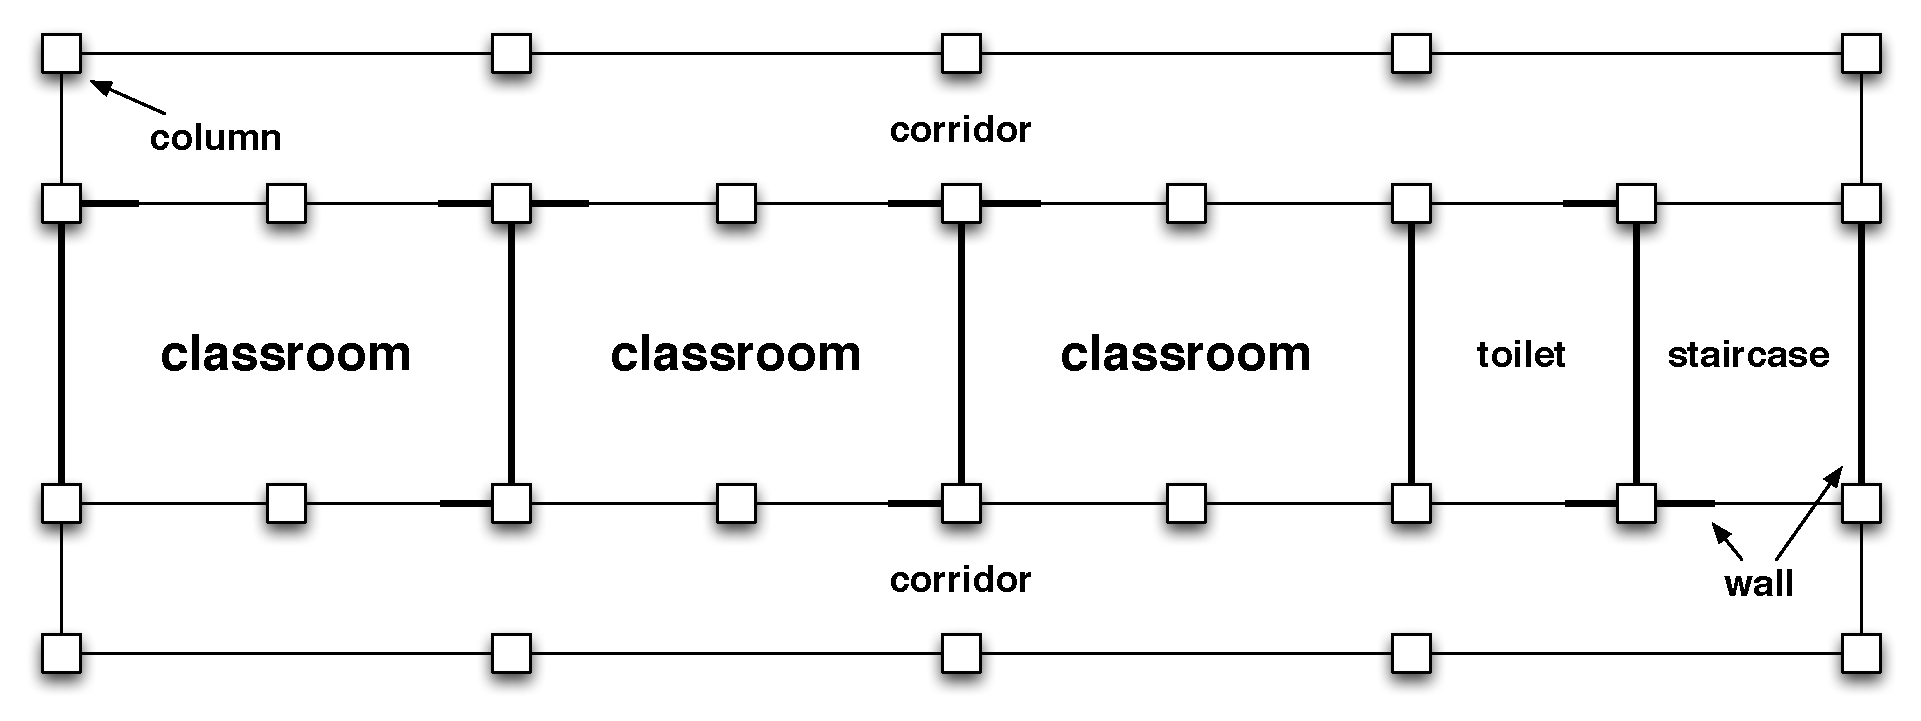
\includegraphics[width=1.0\textwidth]{figures/trad-school-building.pdf}
    \caption{典型校舍} 
    \label{fig:TSB}
  \end{center}
\end{figure}

典型校舍因為其結構形式單純,只需要少量的屬性便可以完整的描述建築物的結構,不用完整詳細的記錄所有的樑柱等構件之個別尺寸強度與位置,只需要紀錄少量的資訊就可以建立出分析用的數值模型,因屬性數量較少,其校舍資料很適合進行各種資料分析的研究,其數量在本國所有校舍當中所佔比例也相當高,而不符合典型校舍特性之校舍,則都歸類為非典型校舍,非典型校舍可能為形狀特殊或是結構規模較大,無法只用少量的資訊就還原出該校舍之結構體的數值模型,因此評估的過程非常仰賴評估人員之專業能力,而校舍耐震資料庫對於非典型校舍則主要在記錄結構物的主要構件的尺寸、分佈、數量等資訊,無法詳實的反映出其特殊的設計,也因此本研究之資料探勘均針對典型校舍進行資料挖掘。

\section{資料收集範圍}

校舍的耐震能力補求流程如圖~\ref{fig:FLOW}~所示。可以分為四個大步驟,分別是校舍普查、初步評估、詳細評估、補強設計與施工,校舍普查主要之目的為全國所有校舍之基本資料建檔,並簡單調查一些主要的設計參數,是由國震中心主導進行,其性質類似於人口普查,是整個計畫中非常重要的基礎建設;接著第二個步驟的初步評估則是根據於校舍普查之基礎,對校舍進行初步評估(preliminary evaluation),其通常的方法是基於結構物之設計及現況填寫評估表,所填寫資料再依評估公式計算出結構物耐震能力之評分等級或指數,此類方法之評估速度快,但是結果可靠度較低,主要的目的是對大量結構物之耐震能力作排序與篩選,這類型評估方法所使用之評估表與評估公式通常是使用已經收集的其他結構物資訊,用數值統計的方法迴歸,或是根據基本的結構耐震能力供需比以及專業人士相關的經驗設計得到的,其所適用之結構物類型也有所限制,評估表並不能套用到各種類型的結構物上;接著經過初步評估後,對於耐震能力有疑慮之校舍,需要進一步進行詳細評估(detailed evaluation),此類方法為對結構物進行詳細的結構耐震分析,通常是使用結構分析程式以電腦數值模擬結構物遇到地震時的非現性行為,並根據模擬結果為依據,準確詳細的檢驗評估出結構物的耐震能力;詳細評估之後,才根據技師的專業判斷,對於耐震堪慮之校舍,依嚴重程度,由工程專業人員,進行結構耐震之詳細評估,倘尚符合補強之經濟效益,即進一步作耐震補強之設計,若不符合補強之經濟效益,則將之列為拆除重建。


\begin{figure}[hbtp]
  \begin{center}
    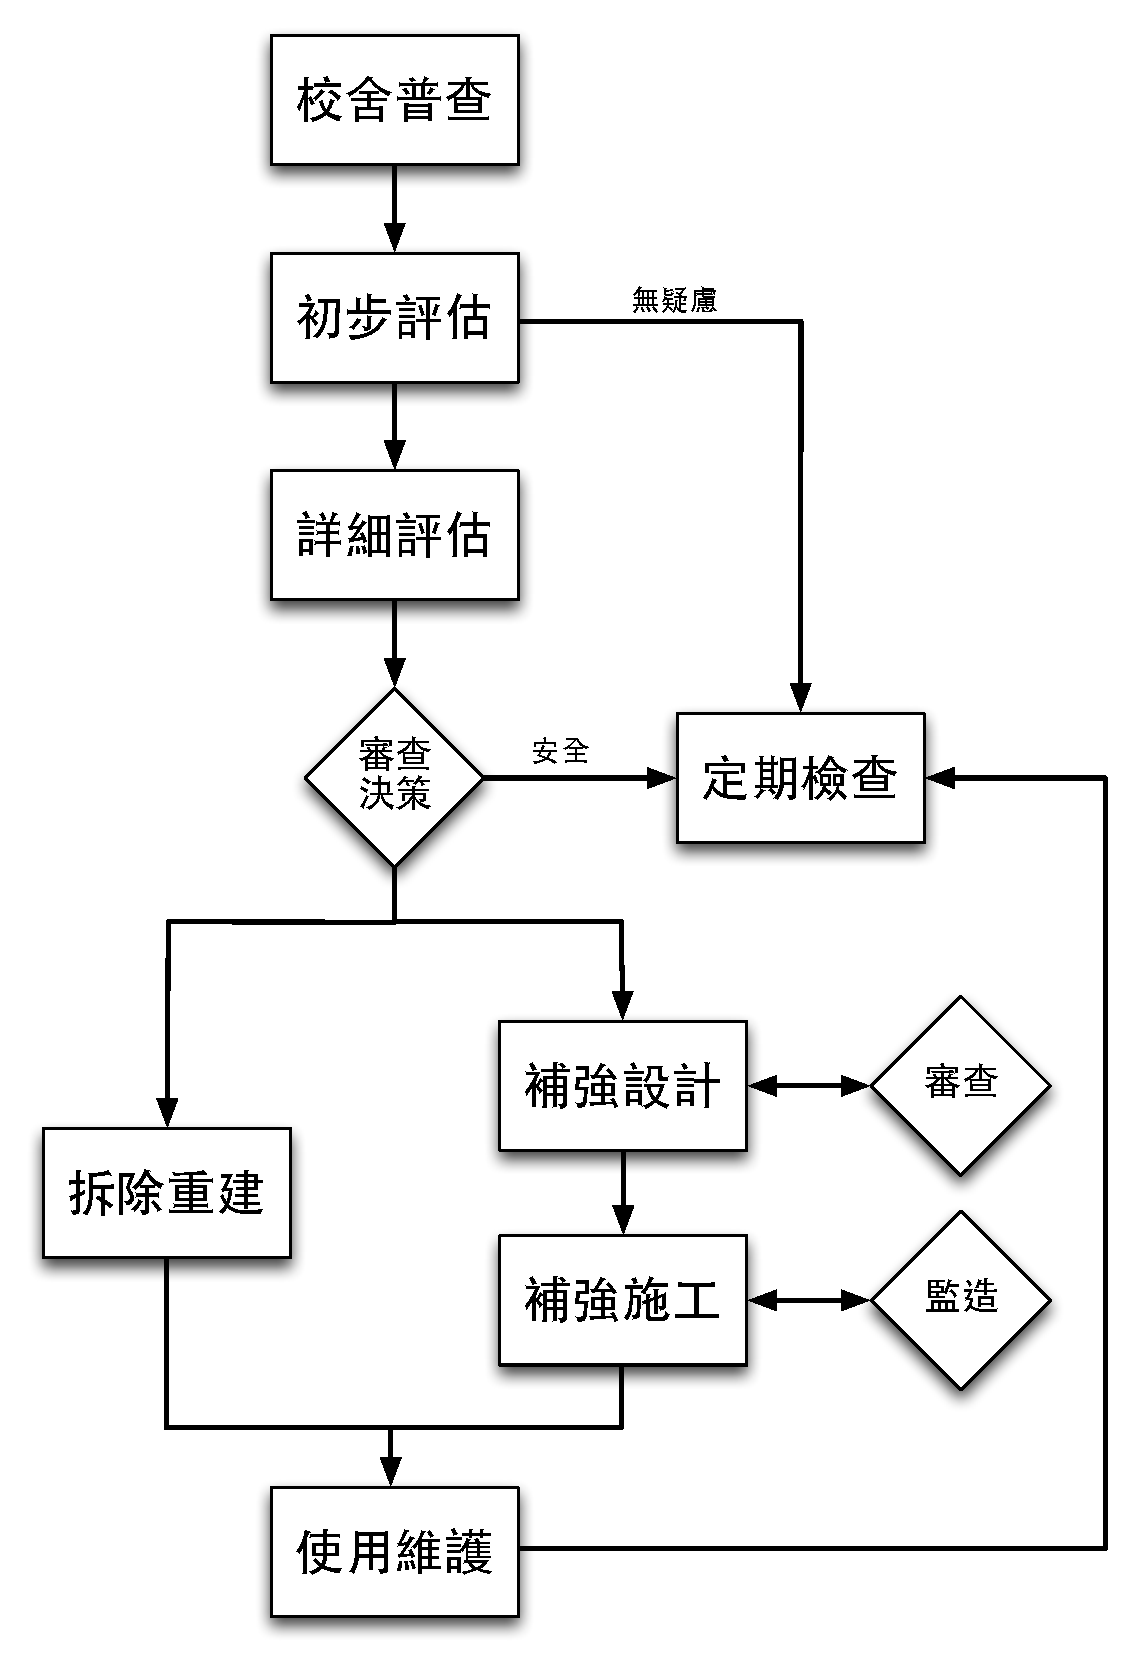
\includegraphics[width=0.8\textwidth]{figures/survey-flow.pdf}
    \caption{評估流程} 
    \label{fig:FLOW}
  \end{center}
\end{figure}

詳細評估方法的可靠度較高,但是花費相當昂貴,所需要的時間也比使用評估表要來的久很多,由於中小學校舍數量龐大,若直接大量投入人力物力,可能造成大量之資源浪費,也無法快速的鎖定耐震能力不足之校舍建築,故針對有效達成此一校舍耐震評估標準需求以及基於上述標準耐震評估程序之精神,國震中心才提出先經由初步評估方法進行篩選的分段式評估方法,有效的將校舍結構之耐震能力排序,以縮小問題之規模,提升整體校舍耐震能力評估作業的效率。

在此過程中會產生的校舍資料最重要的為:初步評估、詳細評估、補強設計、補強工程等四組資料,以下分別介紹四組資料之背景原理及所收集的資訊。

\subsection{初步評估}

詳細評估的原理是分別求取結構物對於地震的需求(demand)和可以承受地震的能力(capacity),然後取其比值,也就是耐震需求比(Capacity Demant Ratio,$CDR$),如果耐震需求比大於~1~則表示建築物的耐震能力足夠,足以承受未來可能發生的大地震。而初步評估雖然是簡化的評估方法,但其原理也和詳細評估相同,是以求得結構物的耐震需求以及耐震能力的比值為目標,其中,耐震需求的部分,是以校舍所在地所可能發生的~475~年週期之最大地震力作為其所需夠能夠承受之地震。至於耐震能力是根據結構物的載重元件尺寸例如牆、柱之斷面積,以及國震中心歸納之公式所推算得到之乘載元件等效強度,求得之值即為校舍之基本耐震性能~$E$,其公式為:

  \begin{equation}E = \dfrac{ 0.354 NF \times (T_{AC} \times T_{AW}) }{(-1 + 6 NF) \times (0.4 S_{aD}) \times Af} \end{equation} 

其中,~$NF$~為樓層數、$T_{AC}$~為柱等效強度、$T_{AW}$~為牆等效強度、$Af$~為總樓地板面積、$S_{aD}$~為一般工址或近斷層區域之工址設計水平譜加速度係數。
求得~$E$~後,還要根據校舍現況及專業人士判斷做調整,調整的方法則是使用國震中心先歸納整理出的調整因子~\cite{ncree03049},總共有六項:

\begin{description}
  \item[平面及立面對稱性($q_1$)]
  本評估表參考建築耐震設計規範之規定,若結構及其側向力抵抗系統的平面幾何形狀具有凹角,超過凹角部分於兩水平方向之結構 尺寸同時大於沿該方向結構總長之~15\%~以上者,表示該結構具有凹角性,則耐震能力折減為~0.95~倍;若該結構具有凹角,但超過凹角部分於任一方向之結構尺寸不足沿該方向結構總長之~15\%~,且無其他平面及立面不規則之情況,則耐震能力不予折減;若該結構不具任何凹角,且無其他平面及立面不規則之情況,則耐震能力增加為~1.05~倍。
  \item[軟弱層顯著性($q_2$)]
  若結構物之一樓因為使用性等考量,而使得二樓以上~RC~牆或磚牆於一樓中斷,致使一樓之極限層剪力強度與勁度降低,將造成地震力作用時變形集中,以致於韌性用盡,建築物就發生軟弱層破壞。故本表格依據牆體中斷的程度折減其對應之耐震能力,若~2/3~以上牆體中斷,則耐震能力折減為~0.8~倍;若~1/3~至~2/3~之牆體中斷,則耐震能力折減為~0.9~倍;若~1/3~以下之牆體中斷,則不折減其耐震能力。
  \item[裂縫鏽蝕滲水等程度($q_3$)]
  鋼筋混凝土構材若具有裂縫,代表混凝土品質不良或強度不足;保護層不足等因素使得鋼筋鏽蝕膨脹,鋼筋鏽蝕將會降低構材之強度,鋼筋鏽蝕膨脹亦會導致混凝土剝落,並加速鋼筋鏽蝕的程度,這些因素都會影響結構物的耐震安全,故以結構物整體之裂縫鏽蝕滲水等程度作為調整項目。若稍有裂縫鏽蝕滲水等情形,則耐震能力折減為~0.95~ 倍;若裂縫鏽蝕滲水等情形較為嚴重,則耐震能力折減為~0.9~倍;若無,則不折減其耐震能力。
  \item[變形程度($q_4$)]
  結構體基礎若有明顯的差異沉陷,將會造成部分構材承受額外的載重,甚至造成嚴重變形,使其耐震能力降低。故若結構體有明顯的變形程度,則耐震能力折減為~0.9~倍;若無,則不折減其耐震能力。
  \item[平面耐震性($q_5$)]
  典型的校舍建築多為數間並排相連,而呈現一字形的平面配置,其走廊形式為了滿足學生活動空間之要求,多將廊柱省略而成為懸臂走廊,故這類校舍結構系統之贅餘度較少。校舍之結構系統贅餘度越多,則於地震時越能發揮韌性與力量重分配的能力,將有助於減少地震時倒塌之可能性,故本研究將典型的校舍建築簡單分為三大類,一為廊外無柱或其他,其耐震能力不予調整;一為單走廊且廊外有柱或中間走廊,其結構系統無懸臂走廊之形式且贅餘度較多,故其耐震能力增加為~1.1~倍;最後一種為雙走廊且廊外有柱,其結構系統贅餘度最多,故其耐震能力增加為~1.2~倍。
  \item[短柱嚴重性($q_6$)]
  一般老舊校舍之柱箍筋間距多為~20cm~至~30cm~左右,其剪力強度不高,且老舊校舍於設計時假設為純梁柱系統,並沒有考慮教室窗台及樓梯廁所等牆壁開氣窗所造成之短柱效應,然而這種短柱效應將會使得剪力容量不足之柱於地震時發生非預期之剪力破壞,導致結構韌性不足,若該校舍有過多之柱受到短柱效應之影響,將易造成校舍瞬間倒塌。故若校舍因窗台或氣窗造成短柱現象之柱根數達到全部柱根數之~50\%~以上,則耐震能力折減為~0.9~倍,若不足~50\%~則不予折減其耐震能力。值得注意的是,短柱嚴重性具有方向性,故評估時只需考慮評估方向之短柱比率是否超過一半即可,另一方向開窗等因素造成之短柱效應不需考慮。
\end{description}


最後乘上調整因子後得到之耐震指標為~$Is$~,其公式如下:

  \begin{equation}Is = E \times \prod_{i=1}^6 q_i \end{equation} 

%  \begin{equation}Is = E \times q1 \times q2 \times q3 \times q4 \times q5 \times q6 \end{equation} 

$Is$~是一個百分制系統,以~80~作為耐震能力堪慮之標準,若校舍調查所得之耐震指標~$Is$~值低於~80~分,表示其耐震能力頗為不足,確有耐震疑慮,若有相當於~475~年週期發生一次之最大地震時,將有嚴重損壞或倒塌之疑慮,應最優先進行耐震能力之補強設計與施工;耐震指標~$Is$~值介於~80~分及~100~分,表示校舍耐震性之安全係數尚不符合耐震設計規範對於此等重要性建築物之耐震需求,仍有耐震性能不足之疑慮,若有相當於~475~年週期發生一次的最大地震時,將有可能發生嚴重結構上之破壞,其耐震能力之提升列為次優先對象;耐震指標~$Is$~值高於~100~分,表示其尚無耐震疑慮,若有相當於~475~年週期發生一次之最大地震時,應不至於發生嚴重結構上之破壞。雖然根據上述耐震指標~$Is$~低於~100~分就須接受耐震能力補強,但根據觀察校舍資料內資料,初步評估結果~90~至~100~分進行詳細評估後,絕大部分都不須進行補強,80~分以下~70~分以上也有一些進行詳細評估後也是裁定不需補強,因此雖然耐震指標~$Is$~不是最後決定補強之最後依據,但也具有相當之影響力。

%初步評估相較於詳細評估的模擬運算而言,是簡化許多的耐震能力評估方式,評估的方式是使用地震中心根據過往資料與相關規範所設計而得,其設計的基礎與詳細評估的 $CDR$ 值相同,皆為校舍的耐震能力與耐震需求的比值,主要的對象為典型校舍,假設校舍之破壞位置為長向的一樓,耐震需求為則為建築物需要能承受其所在地所可能發生的的475年週期最大地震之地震力,由推估的校舍載重以及地震之地表加速度推估而得。而耐震能力則是根據校舍之柱、牆等尺寸,並根據實驗數據推估所得到的等效強度,兩者相除後再乘上調查人員根據校舍現況所填入之調整參數 $Q$,所得到的 $Is$ 即為使用初步評估表格所評估之校舍耐震能力。

\subsection{詳細評估}

美國針對鋼筋混凝土(RC)建築物之耐震能力規範~ATC-40\cite{applied1996seismic}~中,建議用來評估建築物耐震能力之方法稱為容量震譜法(capacity spectrum method),此一評估方法可以分為兩個部分,第一部分是進行側推分析(pushover analysis)取得容量震譜(capacity spectrum),流程如圖~\ref{fig:capacity-curve}~所示,第二部分是根據建築物所在地的各種相關資訊和規範取得需求震譜(demand spectrum),接著使用容量震譜法(capacity spectrum method)以取得建築物性能點,根據性能點座標帶入公式計算可以得到建築物的破壞地表加速度以及耐震能力指標(aseismic ability index),如圖~\ref{fig:performance-point}~所示。

\begin{figure}[hbtp]
  \begin{center}
    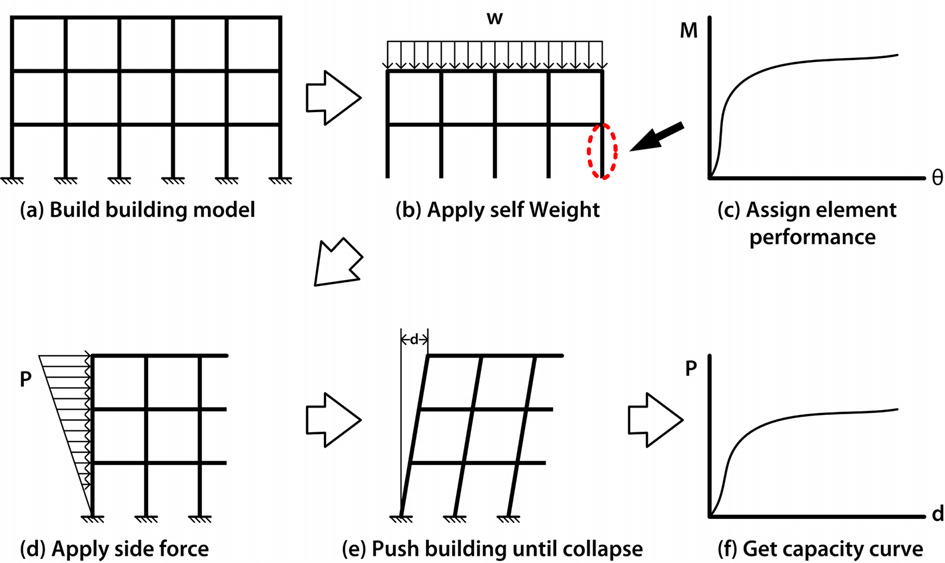
\includegraphics[width=1.0\textwidth]{figures/capacity-curve.png}
    \caption{結構物容量震譜計算流程圖}
    \label{fig:capacity-curve}
  \end{center}
\end{figure}

求取容量震譜的側推分析法需要先建立建築物完整的非線性分析模型,此模型要由進行評估的專業人士根據建築物的幾何尺寸資訊來建立基本的建築物框架。接著根據建築物的材質計算建築物自身重量以及需要承載的人員和配設物件之重量,並將其附加到柱、牆等承載元件上。接著最重要的是設定建築物各構成元件如樑、柱、牆受力時的非線性行為,這些力與變形的關係多為實驗得到或是利用其他分析模擬方法得到的。至此,側推分析要用的數值模型才算建立完成。而側推分析其程序是依照~FEMA-440\cite{fema440}~
之建議,逐步地給結構模型施加增量的側向外力,將結構物向某一方向推動,每次增量即進行一次結構分析計算每一構件之應力與變位,之後與上一次的分析結果累加即可得到每一個構件於此受力階段之反應,並判斷構件是否破壞,例如開裂、降伏,甚至達到極限強度,之後各構件依其破壞程度更新其行為,例如改變其勁度,或者將已發生破壞的構件從結構模型中抽離,如此重複分析直到結構不穩定而崩垮為止,側推分析完成後可以得到建築物之容量震譜。

需求震譜是根據建築物環境現況,參考規範製成之地震需求頻譜。參考的環境狀況如土層種類,堅硬的土層可以讓建築物有較好的抗震能力。另外靠近斷層的建築物在地震發生時往往會因為斷層於地震時產生的反應而受到嚴重的損害,因此建築物與斷層的距離也納入參考的資料之一,稱為近斷層效應(special effects of near-source earthquakes),其他還需要的資料有地層資料、地震震區等,綜合這些資料並參考規範即可得到該建築物所需符合之需求震譜。

\begin{figure}[hbtp]
  \begin{center}
    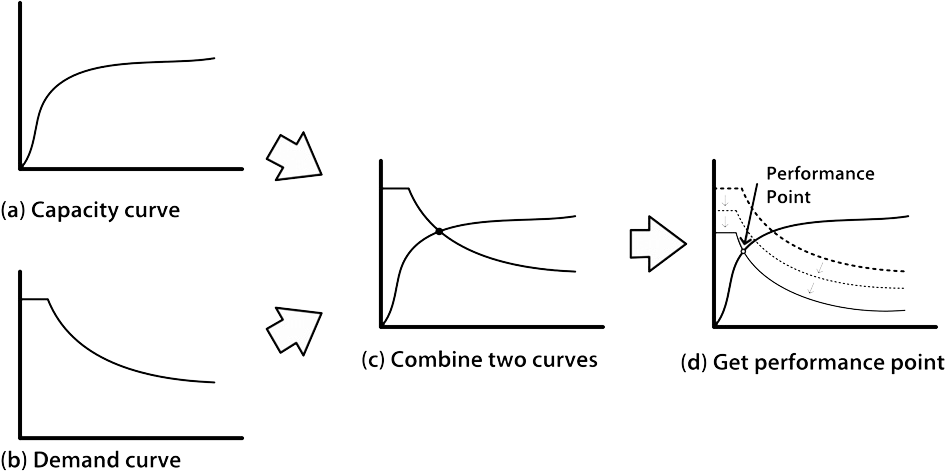
\includegraphics[width=1.0\textwidth]{figures/performance-point.png}
    \caption{結構物性能點計算流程圖}
    \label{fig:performance-point}
  \end{center}
\end{figure}

容量震譜法(capacity spectrum method)最後是將需求震譜以及容量震譜轉換格式後相疊,求取建築物之性能點(performance point),性能點之物理意義為該建築物在特定水準地震下所能承受之最大變位及剪力,但是由於結構物受地震力作用進入非線性行為時,結構物的阻尼效應會產生消能的作用,因此還要視情況對需求曲線進行折減,此為一個迭帶運算的過程,可能需要不斷折減需求曲線,並進行性能點正確性的檢核,直到檢核通過,才能得到建築物真正之性能點如圖~\ref{fig:performance-point}~,由建築物性能點之座標帶入公式可以求得建築物的破壞地表加速度(collapse ground acceleration,~$A_C$),詳細評估所使用的耐震能力值為耐震需求比($CDR$),其定義如下:

\begin{equation} CDR = \dfrac{A_C}{A_D} \label{eq:CDR}\end{equation} 

$A_D$~為根據建築物所在地的並依據規範所得到的,建築物所需要能承受的~475~年週期最大地震所產生之地表加速度,$CDR$~大於~1~代表此一棟建築物能夠承受該地區~475~年一遇的最大地震。

\subsection{補強設計與竣工資料}

如果校舍經過詳細評估過後,負責的專業人士認為此棟校舍確實有安全疑慮,但尚可以補強,不需要拆除重建時,則該棟校舍就會進入補強設計階段,此一階段的工作也是委託專業人士執行,負責的專業人士需要依據詳細評估的結果,設計出兩種不同的補強方案,並且對不同的補強方案進行詳細的耐震能力評估,因此這個階段的資料包括兩組補強設計的資料,以及兩組補強後的耐震能力詳細評估資料。補強設計收集的資料主要為使用的補強工法以及補強量,主要收集的補強工法包括了六類:增設構件、柱補強、牆補強、樑補強、減載措施、基礎補強。

增設構件所可能增加的構件包括了剪力牆、翼牆、斜撐、柱、樑等,皆為結構物之乘載構件,其優點是可以有效且直接的增加結構物的乘載能力,缺點是增加的構件可能讓結構物的隔間變化,讓使用功能性變差。而另外一種補強方式則是在現有的構件上加強,包括了柱補強、牆補強、樑補強,這三種補強工法都是針對現有的結構元件加強,例如擴柱、鋼板貼片、複合材料貼片等,這類方法不改變節結構之基本設計,對於結構物之使用性影響較小,但仍然可能影響到建築物之採光、通風等。減載則是屬於比較消極的補強方式,藉由減少結構物的乘載重量來檢少結構物受到地震力作用而倒塌的可能性,而其措施包括了拆除樓層,通常為從上往下拆除、樓層數則是專業人士評估判斷,另一種方式則是變更用途,如果校舍結構物對於自重本身的乘載能力已經足夠,則可以考慮改變部分樓層的用途,減少其所需要乘載的載重,而減載措施相較於其它幾種補強方式,是屬於成本較低的補強方式。

補強設計階段,負責設計的專業人士會提出不同的補強方案做為校舍補強工程的參考,而後根據預算和學校單位的需求以及校舍安全性等因素綜合考量以決定補強方案,並進行補強工程,在工程完成後,國震中心還會收集相關的資料,包括補強方法、補強構件的數量、不同類型工程之花費、補強材料強度報告等,而在這些資料當中,補強工程的經費是一個非常重要的數據,因為此一資料數值是校舍補強流程當中最後一個階段才會得到的,但卻是在整個校舍補強計畫當中,初期編列預算就非常需要,影響很大的數據。

\section{資料庫結構}

此一校舍耐震資料庫使用的是用途非常廣泛的關連式資料庫,其實體關係圖如圖~\ref{fig:school-er}~所示,實體關係圖是在初步設計資料庫結構時所用,可以呈現關連式資料庫中各資料表間的關係,使用的呈現方式是實體關聯模型(ER model),此一資料模型是透過實體(entity)與關係(relation)兩種物件來作表示,實體是所欲儲存資料於現實中之實際物體,關係則是各實體間的關係,設計之結果可以用實體關係圖之形式表示,實體關係圖則以矩形代表實體、菱形代表關係、橢圓形代表實體的屬性。


\begin{figure}[hbtp]
  \begin{center}
    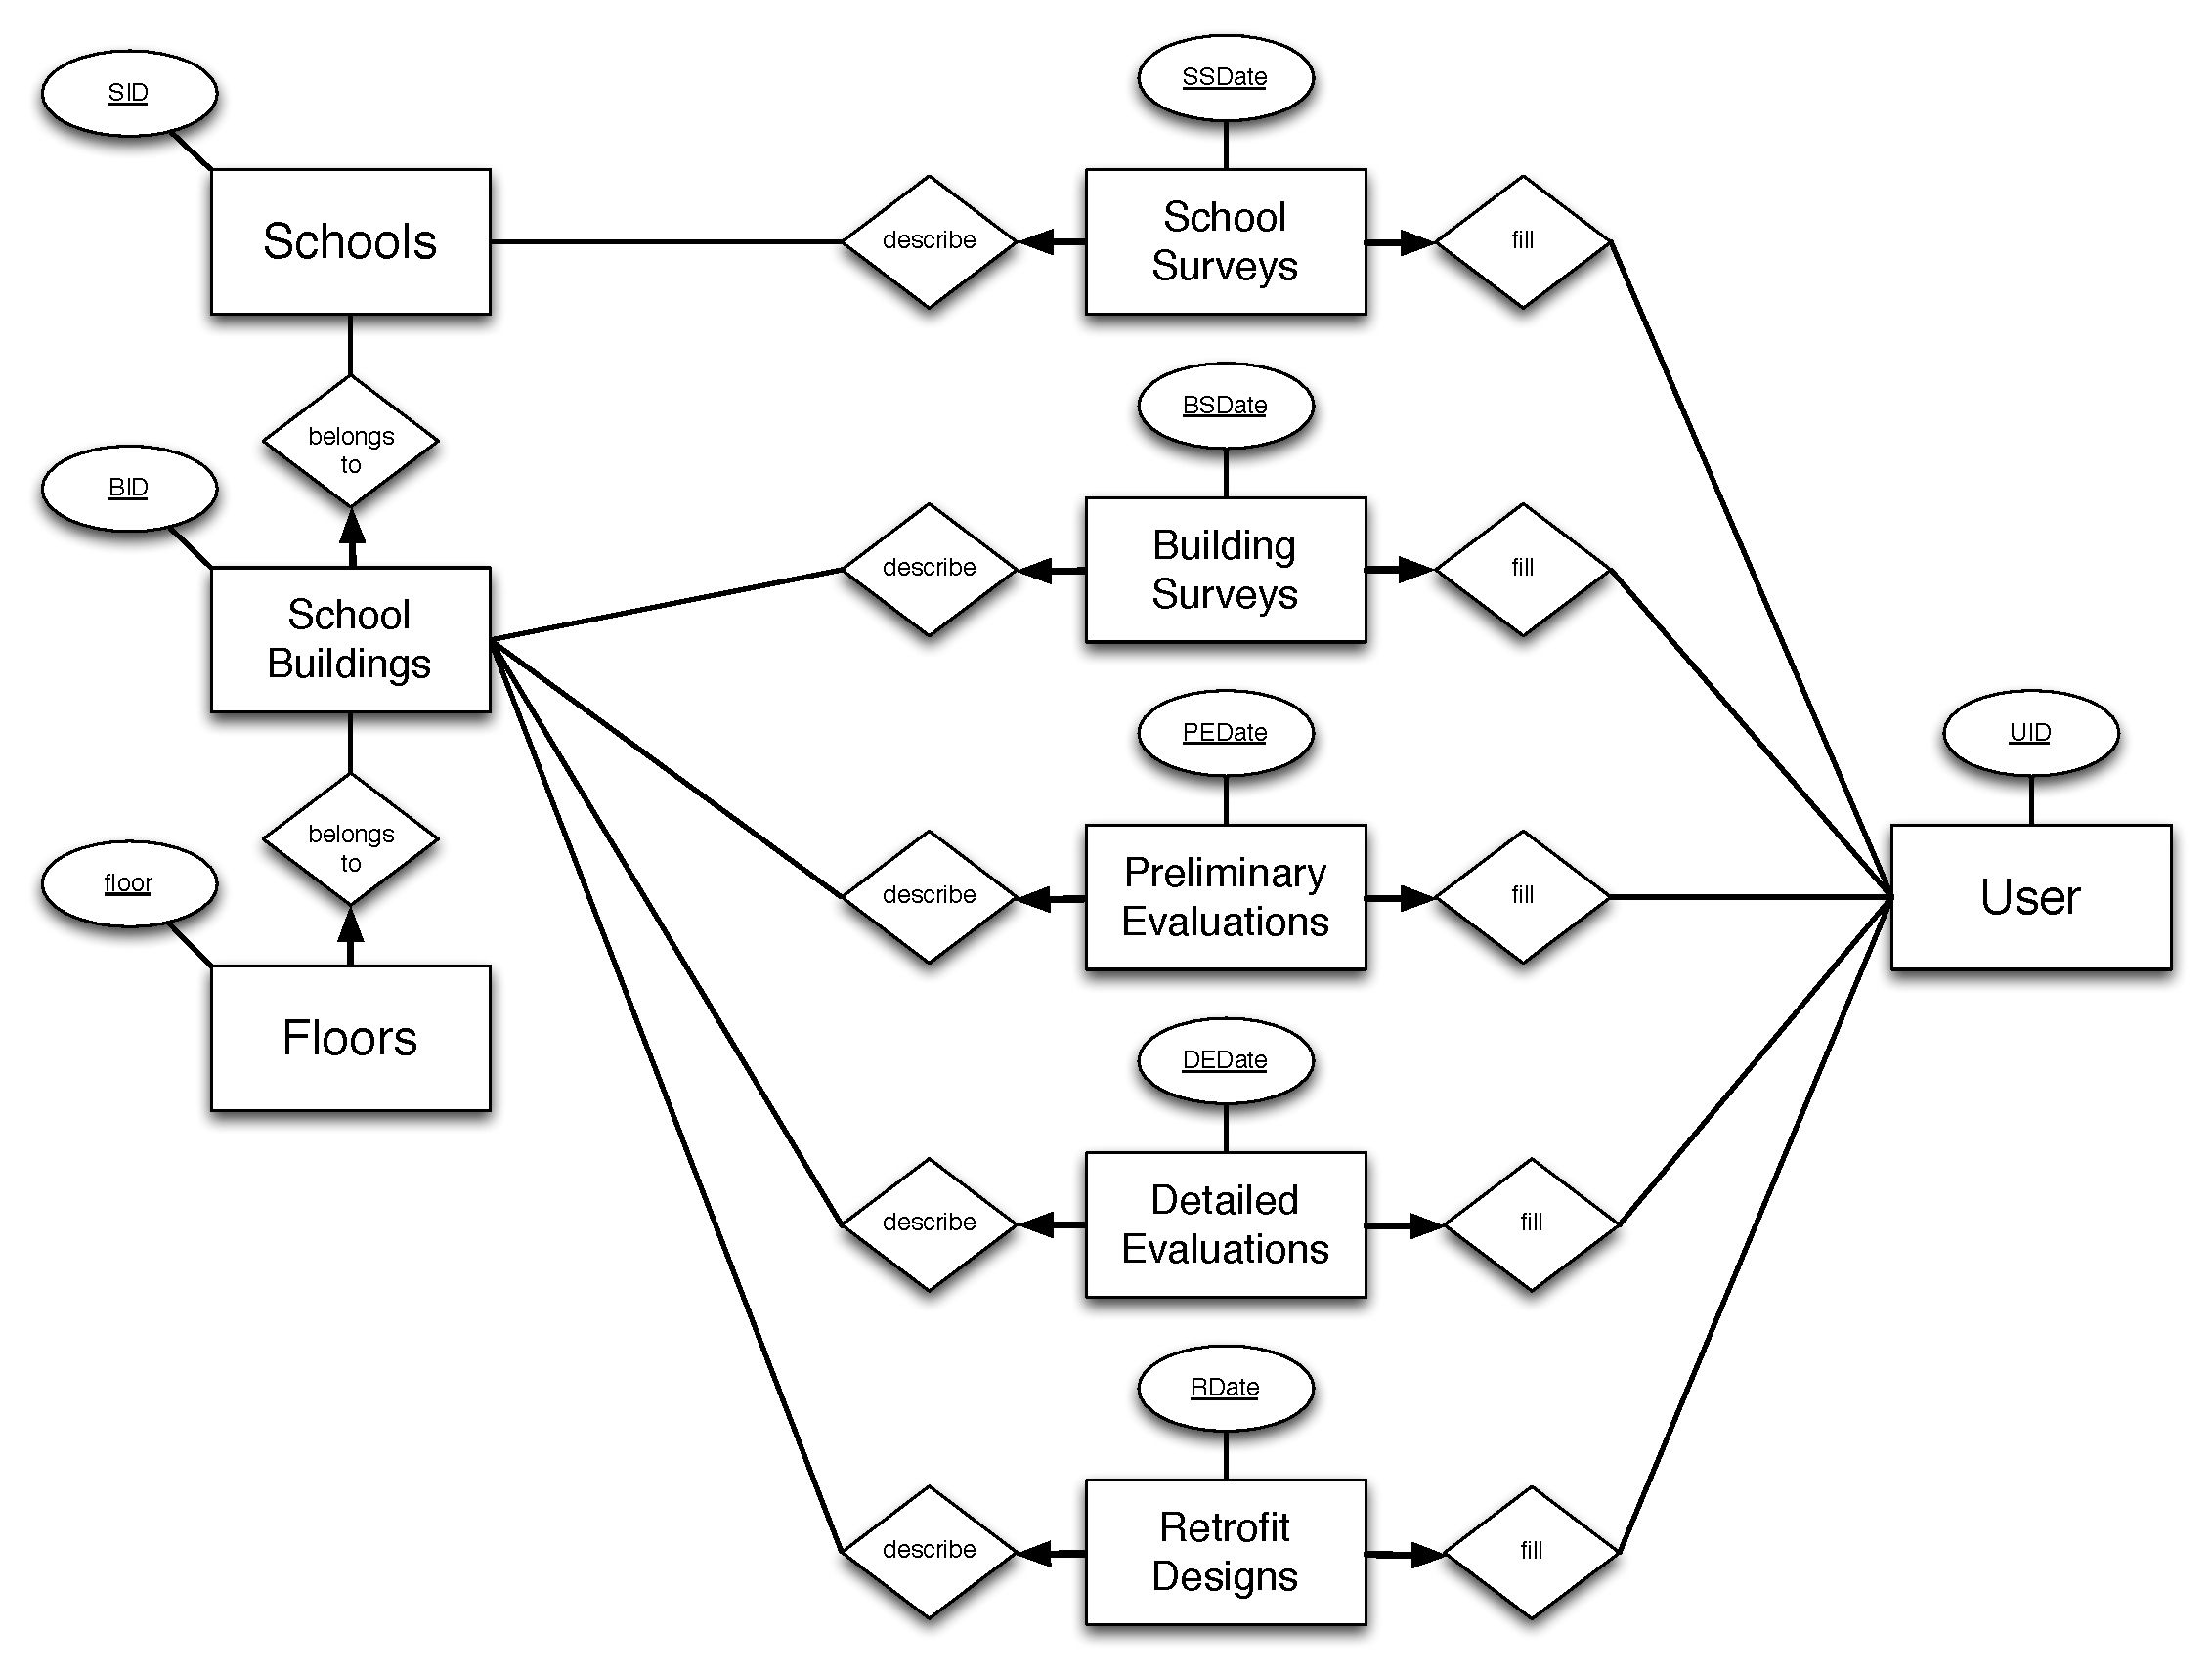
\includegraphics[width=1.0\textwidth]{figures/school-er.pdf}
    \caption{校舍耐震資料庫實體關係圖} 
    \label{fig:school-er}
  \end{center}
\end{figure}


圖~\ref{fig:school-er}~之標示採簡化之表示法,即各表格之屬性(attribute)只標示出其主鍵(primary key),校舍耐震資料庫的基礎是~School~和~School Building~兩個資料表,Schools~代表所有學校基本資料集合之實體組(Entity Set),構成~Schools~之每個實體(Entity)均是代表某學校,資料庫系統是以紀錄了此學校的基本資料,包含學校名稱、地址、GPS~座標等資訊為屬性,而~School Buildings~代表所有校舍集合之實體組,構成~School Buildings~之每個實體均是代表某學校之某校舍,每棟校舍是以紀錄其之校舍名稱、建造年代、設計圖等資訊為屬性,因每一間學校內多有多棟校舍,故其與~Schools~間為一對多之關係,而與校舍的樓層數為不定數量,故把樓層相關之資料屬性獨立出來存放在~Floors~資料表,其代表所有樓層集合之實體組,構成~Floors~之每個實體均是代表某學校某校舍之某一樓層,每層樓是以儲存該樓層之樓高、樓地板面積、教室間數這類各樓層獨有之資訊,由於每棟校舍均有多層樓,故其與~School Buildings~為一對多之關係。

有了以上的基礎後,資料表設計便基於圖~\ref{fig:FLOW}~之流程,將不同階段的調查表、評估分為不同之資料表。圖中之~School Surveys~方塊即表所有簡易調查集合之實體組;構成~School Surveys~之每個實體均是代表對某學校所作之某次簡易調查,每次調查是以紀錄學校整體之損害狀況等調查資料為屬性代表之,由於某學校之狀況會隨時間改變,學校之調查會定期重新調查,故其與~Schools~間為一對多之關係,此假設同一日不會有兩次的調查,故其與~School Surveys~不另設獨有的~ID~為主鍵,而是採~SID(調查學校)與~SSDATE(調查日期)之組合;構成~Building Surveys~之每個實體均是代表對某學校之某校舍所作之某次簡易調查,其即以該次調查所填調查表格之資料為屬性代表之;構成~Preliminary Evaluations~之每個實體均是代表對某學校之某校舍所作之某次初步評估,其即以該次評估所填評估表格之資料為屬性代表之,Detailed Evaluations~實體組代表詳細評估之集合;Retrofits~實體組則是補強設計之集合,而後續包括補強施工和竣工報告等都與~School Buildings~實體。此四個實體組與校舍間如同~School Surveys~與~Schools~間之關係,由於每棟校舍均可能於不同時間進行不只一次,故其與~School Building~間關係為一對多關係。Users~實體組代表所有填表人之集合,系統是以紀錄某填表人之簡易資料,包括姓名、聯絡方法、職稱等為屬性代表之,因為一個填表人可能負責評估多間校舍,故~Users~與上述四個代表評估調查之實體組間之~fill~關係組也為一對多之關係。








	\renewcommand\thetable{\arabic{chapter}-\arabic{table}}
%\renewcommand\thefigure{\arabic{chapter}-\arabic{figure}}
\renewcommand{\theequation}{\arabic{chapter}-\arabic{equation}}
\chapter{資料探勘與探勘目標分析}
\label{cha:data-mining} 

過往在各種不同商業、工業、學術等領域都隨著產業逐步的數位化,有各種資料庫甚至資料倉儲系統的建置與資料收集,例如零售業的交易紀錄,各種學術實驗的結果記錄等等,而隨著時間推移,這些資料庫和倉儲系統收集的資料數量都成長的非常龐大,資料間的關係和複雜度也越來越複雜,這些資料除了當初建置的目的和資料的統計分析外,研究人員還開始思考更進一步的資料應用,希望能把資料中以往隱藏不可見的知識找出來,因此資料探勘(data mining)此一研究領域就因應而生。應用在資料探勘研究的演算法非常多種,包括統計、人工智慧(artificial intelligence)、機器學習(machine learning)、模式識別(pattern recognition)等,只要能夠用來在大量資料中尋找有用知識的方法,都可以作為資料探勘的演算法。

而資料探勘的結果優劣,除了演算法和欲解答問題間的契合度之外,整體資料探勘流程中,不同階段工作執行的品質也是很重要的因素,資料探勘的流程在不同領域有各種不同的規範,其中最廣為被使用的是~CRISP-DM\cite{shearer2000crisp}(Cross Industry Standard Process for Data Mining)這個跨領域的資料探勘流程,其是由~SPSS~以及~NCR~兩大廠商在~1990年開始發展的,它的流程架構如圖~\ref{fig:CRISP-DM}\cite{crispdmdiagram}~所示,將一個完整的資料探勘流程分為六個步驟,分別為:

\begin{figure}[hbtp]
  \begin{center}
    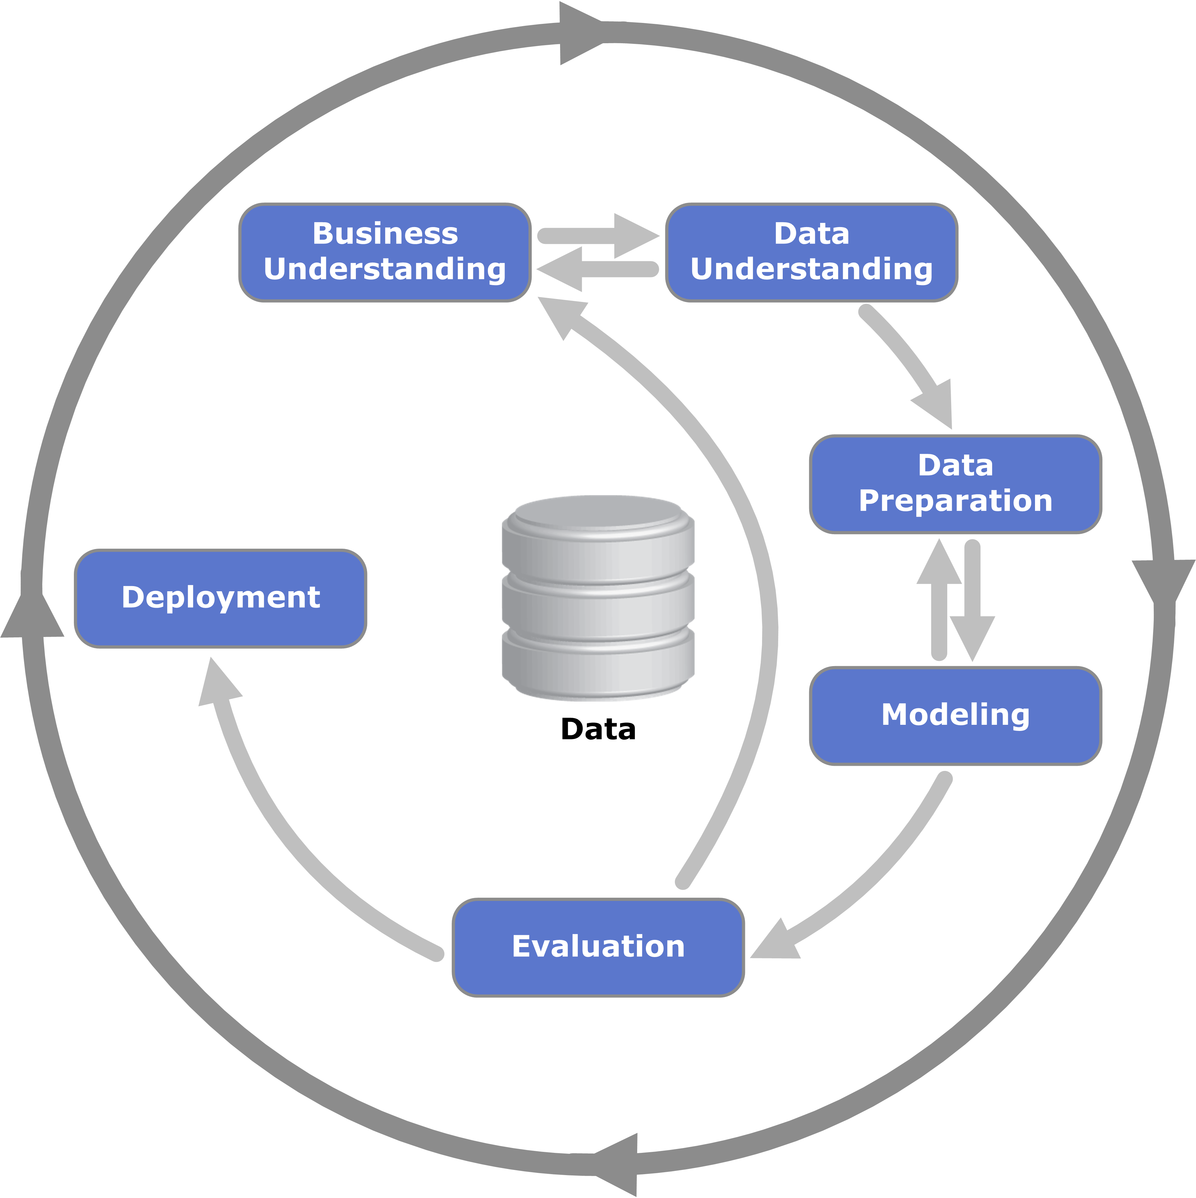
\includegraphics[width=1.0\textwidth]{figures/1196px-CRISP-DM_Process_Diagram.png}
    \caption{CRISP-DM 流程圖 (c)Kenneth Jensen, CC BY-SA 3.0} 
    \label{fig:CRISP-DM}
  \end{center}
\end{figure}

\begin{enumerate}
\item \textbf{定義領域問題}(Business Understanding):CRISP-DM~所定義的資料探勘步驟第一步要將希望解答的問題瞭解並定義清楚,有清楚明確的問題定義,才能夠規劃出需要收集哪些資料,用哪種類型的資料探勘方法來挖掘知識,解答問題。
\item \textbf{定義分析資料}(Data Understanding):有明確的問題定義之後,就能夠更深入的探討有哪些相關的資料,要解答此一問題所需要的相關資料為何,並且實際的去收集這些資料。
\item \textbf{資料前處理}(Data Preparation):此一步驟是資料探勘流程當中,相當重要的一個步驟,對於模型的品質優劣會有相當大的影響。會需要資料前處理的原因主要有兩個,第一個原因是由於現實世界的資料都會有很多雜訊在其中,像是人為輸入的錯誤、較為極端的離群案例資料等,因此在真正的訓練並建立模型之前,需要先把這些雜訊去除,這些雜訊在資料庫中的呈現通常為缺漏值、過大或過小的數值或是意義上不合常理的數值;另一個原因則是要將不同的輸入屬性的數值作整理,讓不同的資料探勘演算法可以更容易的根據不同屬性的特性來建立模型,這些前處理的方法包括了數值正規化、取指數對數、單位調整甚至是重新組合出新屬性,像是主成分分析法。
\item \textbf{建立模型}(Modeling):選擇適合該問題的資料探勘方法對前處理過的資料進行分析與模型建立,模型之建立工作包括了適合演算法的挑選以及不同演算法參數之挑選,兩者都是需要不斷嘗試並調整的工作。
\item \textbf{評估模型}(Evaluation):評估前兩步驟中所建立的模型品質是否符需求,並且要避免過適(overfitting)的現象,實務上是將資料分為訓練集與測試集兩組來驗證模型的可靠度,更為嚴謹的分析可以使用十群交叉驗證方法來處理,判斷的依據則根據不同的資料探勘方法有不同的模型品質指標,例如決定係數、線性關係、正確率等等。
\item \textbf{應用模型}(Deployment):將模型產出的知識實際納入應用,抑或是將探勘結果整理成完整的報告。
\end{enumerate}

其中資料探勘在收集完資料後的大部分的工作,均在資料前處理以及建立模型兩個步驟,此二步驟的操作對於最後產出模型之品質有相當大的影響。而本研究之流程較~CRISP-DM~之流程稍有不同,是先基於一個現有的特定領域的校舍耐震資料庫作分析,找出校舍耐震資料庫中各種潛藏知識的可能性,定義出這些知識所能夠解決的問題,詳細分析問題的需求,之後則是照著~CRISP-DM~的流程進行,從校舍耐震資料庫中挑選出相關的資料屬性,然後接著進行資料前處理、建立模型、評估模型幾個步驟。

資料探勘技術方法繁多,Fayyad~\cite{fayyad1996data}根據其處理的問題形式,將資料探勘的方法分為分類、分群、迴歸以及關聯等四種主要的問題類型。其中,分類方法處理的問題是用來判斷資料的類別,而且這些類別是已知的類別,例如將所有的校舍資料分類成有安全疑慮和沒有安全疑慮的方法就是屬於分類問題。分群問題和分類問題有點相似,一樣是將資料分成數個群組,最主要的差異是分群問題的各個群組的特性在一開始並不清楚,分群方法是將資料根據其屬性數值為依據,分析其相似度,把相似的放在同一個群組,不同群組的特性是要在分出群組後才能夠進行分析瞭解的。迴歸問題就是要用迴歸方法來從資料的屬性中,找出特定屬性與其他屬性間的關係模型,這些屬性間的關係可能是非線性的,而且沒有解析解的關係模型,因此常見的方法是用統計的方式,從現有的資料來反向歸納出關係方程式,又或著是用像類神經網路之類的機器學習方式,透過現有的資料來讓機器學習以求出關係模型,以校舍耐震資料庫來說,校舍耐震能力指標的預測就是一種迴歸問題,校舍耐震能力指標與其校舍的設計參數間的關係就是一個非線性關係,要得到兩者之間的非線性模型就需要用到回歸問題的分析方法,迴歸問題也是最常見的資料探勘問題種類。最後一種是尋找屬性間的關聯,這種問題的主要目標在尋找不同筆資料屬性間所存在的關係,舉例來說,使用校舍耐震資料庫的資料來作關聯分析,可能可以去尋找像是:五層樓的校舍的校舍長度深度有什麼趨勢,或是民國八十到九十年之間所建校舍的校舍走廊設計是否偏好有走廊柱等。本研究在定義好所欲解答的問題後,根據問題的性質判斷,使用的資料探勘方式以迴歸為主,分類分群的方法則是為輔助。

以下分別介紹本研究所使用到的各種分析方法,除建立模型的各種訓練和學習演算法外,還包括資料前處理和驗證所使用的分析方法以及驗證指標。


\section{資料前處理方法}

資料前處理方法常見的目的有:找出重要性較高的屬性、凸顯資料特性、剔除特異資料點等;本研究主要的資料過濾方法為資料的合理性分析,其是根據資料特性,根據經驗與專家意見等參考依據,建立出資料合理性的判斷方法。而除了合理性分析外,尚有較為簡單的數種方法,包括:

\begin{itemize}
\item 輸入屬性篩選
\item 子資料集挑選
\end{itemize}

輸入屬性篩選的主要目的在剔除和探勘目標不相關的資料屬性,減少資料維度,可以讓機器學習的效率更好;子資料集挑選是針對特定屬性,如果有非常不平均之分佈情形,例如一個二元指標,有很大比例的資料之值都相同,那就可以透過子資料集挑選的方法,將這一大類的資料挑出,和輸入屬性篩選一樣可以減少資料的複雜度。而除了以上的三種前處理方法外,還有主成分分析法,是透過數學統計分析求得最能夠代表資料變異的屬性。

\subsubsection{主成分分析}

主成分分析(Principal Component Analysis, PCA)是常見的前處理方法,它可以用來減少資料的維度,其數學原理是將資料向量投影到不同的座標系統,將原始的資料轉換成不同座標系的的向量資料,且能保持最大程度的,輸入屬性對於輸出屬性的貢獻,如圖~\ref{fig:pca}\cite{ben2013pca}~所示,在一個~X~Y~座標系統中分佈的資料點,可以透過~PCA~分析,找到兩個更能夠代表資料特性的屬性座標軸~$\sigma^2_{signal}$~和~$\sigma^2_{noise}$。

\begin{figure}[hbtp]
  \begin{center}
    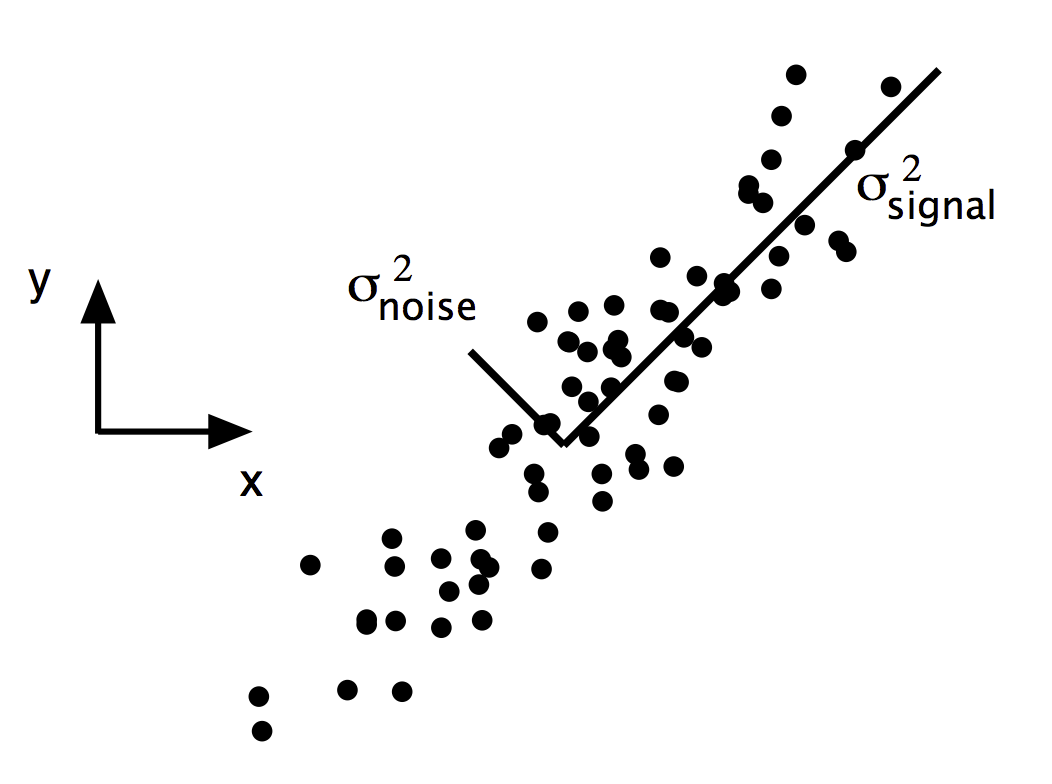
\includegraphics[width=0.6\textwidth]{figures/pca.png}
    \caption{主成分分析原理} 
    \label{fig:pca}
  \end{center}
\end{figure}


% PCA, a very common data preparation method, can identify very important attributes among various attributes. The goal is to convert the original variables through vector transition into mutually independent variables of a linear combination. The ideal situation is that principal components obtained from linear combination retain most of the information of original variables.

\section{資料探勘方法}

資料探勘的方法分為分類、分群、迴歸以及尋找關聯~\cite{fayyad1996data}~,其中迴歸是最常使用到的一種,本研究的主要目標皆可以歸納為迴歸類的問題,因此使用到的迴歸演算法最多,接著才是作為輔助用的分類和分群演算法。

迴歸、分類、分群三種資料探勘所建立的模型可以簡單的定義為:

\begin{equation} y = f(x) \label{eq:ModelEqu}\end{equation} 

$f(x)$~就是透過資料探勘分析學習而得到的模型函數,~$x$~代表輸入參數,輸入參數是各種已知的屬性資料,例如可以簡單透過量測得到的校舍尺寸資訊,~$y$~則是代表輸出參數,也就是希望透過這個模型所得到的,比較難取得的屬性資料,例如需要經過詳細評估才能的到的校舍~$CDR$~值、或是校舍分類的類別索引。

\subsection{迴歸方法}

\subsubsection{Generalized Linear Model}

廣義線性模型是由Nelder and Wedderburn~\cite{citeulike:5485398}所提出,比起迴歸分析(simple regression)更為彈性,此模型是假設資料點的分佈有一分佈模式,且輸入參數~$x$~與輸出參數~$y$~之間的關係是由一連結函數(Link Function)建立,如~log function、power function~等,其定義之~$x$~與~$y$~間之關係模型如下:


\begin{equation} g(E(y)) = x\beta + O, y \sim F \label{eq:GLM}\end{equation} 

$g(.)$是為所選的鏈結函數,$E(y)$~是~$y$~的期望值,~$O$~是偏移(offset)變數,~$F$~則是~$y$~的分佈模型,其是用牛頓法(Newton-Raphson Method)不斷的調整~$\beta$~使的~$x\beta + O$~逼近~$g(E(y))$~,最後最接近的方程式即為~$x$~與~$y$~兩者的關系式。比起迴歸分析,此方法還需要了解~$y$~值分佈狀況,選擇出最適合的分佈函數,並假設~$x$~與~$y$~間的鏈結函數形式,雖然越多的參數選擇代表了更多的模型不確定性,但廣義線性模型卻能夠提供比迴歸分析更廣的應用範圍,也可能得到更接近真實的關係模型。


\subsubsection{類神經網路}

類神經網路(Artificial Neural Networks,ANNs),其是希望能模擬建構出人腦內的神經網路,以處理各種複雜的問題,人類大腦是由大約千兆個神經元(Neuron)所構成,而每個神經元又會和其他約一萬個神經元連結,構成一個龐大且複雜的神經網路,這樣複雜的一個神經網路讓人類可以學習並了解各種事物與知識。McCulloch and Pitts~\cite{mcculloch1943logical}所提出的模型為後續類神經網路發展的雛形,而目前最為被廣泛使用的類神經網路結構為倒傳遞類神經網路(Back-Propagation Network, BPN),為一種監督式學習網路,應用十分廣泛。Werbo~\cite{werbos1974beyond}首先提出隱藏層及倒傳遞學習理論的概念,但在當時並未受到重視。直到~Rumelhart~及~McClelland\cite{rummelhart1986learning}於~1986~提出~BPN~學習演算法及通用差距學習法則(Generalized Delta Learning Rule),採引起學者的廣泛討論。倒傳遞演算法是將一組樣本~1/0~問題變為一個非線性最佳化的問題,其基本原理是利用最陡梯度下降法(Gradient Steepest Descent Method)以計算且調整網路權重,使推論輸出值與目標輸出值間的誤差最小化,得到精確的學習。因此,倒傳遞類神經網路是用於診斷與預測上,若將此模式視為輸入與輸出間的映射關係,則~BPN~演算法是一種輸入輸出的映射過程,一個標準的~BPN~類神經網路可以分為輸入層(input layer)、隱藏層(hidden layer)、輸出層(output layer),其結構如圖~\ref{fig:ANN-network}\cite{larose2005discovering},分別介紹三種神經元如下:

\begin{description}
  \item [輸入層神經元]
  用以表現網路的輸入變數,其處理單元數目依問題而定,通常相等於所使用的輸入參數,使用線性轉換函數,即~$f(x)=x$。
  \item [隱藏層神經元]
  用以表現輸入處理單元間的交互影響,其處理單元數目並無標準方法可決定,經常需以試驗方式決定其最佳數目,使用非線性轉換函數,網路可以不只一層隱藏層,也可以沒有隱藏層。
  \item [輸出層神經元]
  用以表現網路的輸出變數,其處理單元數目依問題而定,使用非線性轉換函數。
\end{description}

\begin{figure}[hbtp]
  \begin{center}
    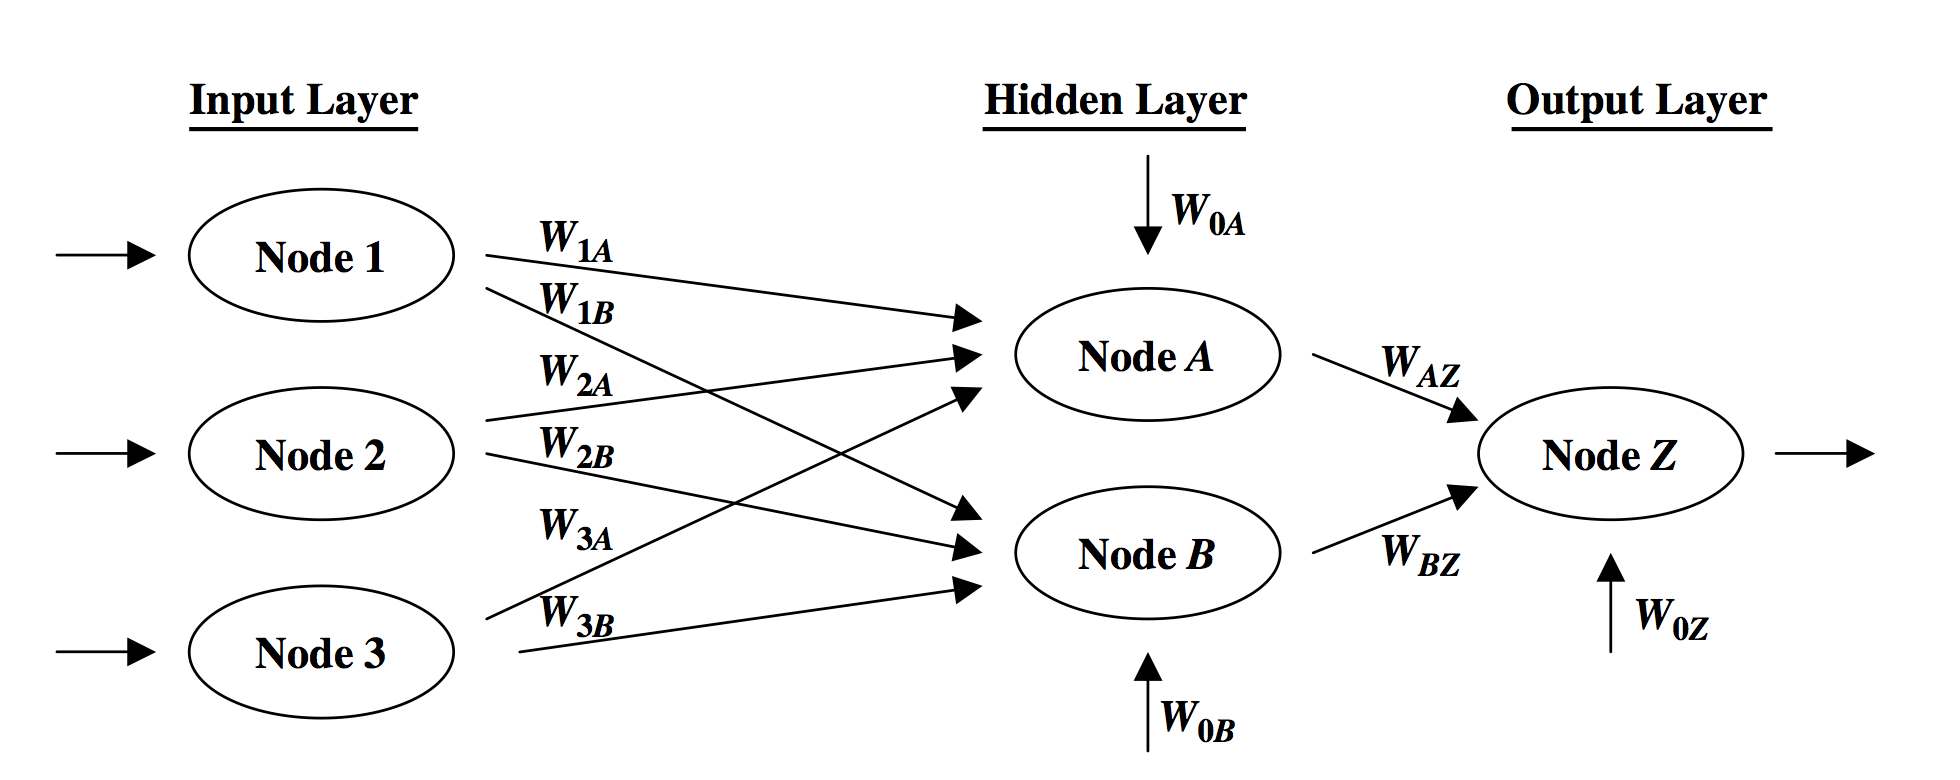
\includegraphics[width=1.0\textwidth]{figures/anns-network.png}
    \caption{類神經網路結構圖} 
    \label{fig:ANN-network}
  \end{center}
\end{figure}

處理單元其輸出值及輸入值的關係式,一般可用輸入值的加權乘積和之函數來表示:

\begin{equation}\begin{split}  Y_j &= f(net_j) \\ net_j &= \sum W_{ij}X_i - \theta_j \label{eq:anns}\end{split}\end{equation} 

其中,$Y_j$~為輸出層第~$j$~個處理單元之推論輸出值,$net_j$~為輸出層第~$j$~個處理單元之集成函數,$W_{ij}$~為第~$i$~個輸入層單元與第~$j$~個輸出層單元間之連結權重。$X_i$~為輸入層第~$i$~個處理單元之輸入值。$\theta_j$~為輸出層第~$j$~個處理單元之閥值,$f$~為轉換函數,是為神經元從輸入層加總轉換至輸出的一種映射規則亦是將非線性的影響導入網路中的一種設計。而轉換函數的選擇相當多, 本研究採用的轉換函數為對數雙彎曲函數,如下所示:

\begin{equation} f(x) = \dfrac{1}{1 + e^x}  \label{eq:annsf}\end{equation} 


\subsubsection{基因規劃}

基因規劃(Genetic Programming,GP)是基於基因演算法(Genetic Algorithm, GA)發展而來,而~GA~是~1975~年由~John Holland\cite{holland1975adaptation}~所提出的演化求解方法,其是基於生物演化的過程為基礎,假設問題的目標可以轉換為二元的基因序列,再透過模擬生物交配、突變的進化過程,求得最佳化問題的解,和傳統的演化求解方法相比,基因演算法可以比較容易的找到全域最佳解,且其可以快速的找到足夠好的解,即使問題的複雜度很高。基因演算法的應用領域相當廣泛,在營建領域也有不少的應用,Huang...et. al.\cite{minshui2009study}~就使用GA預測梁模型受力後會產生破壞的位置及其嚴重性,Šešok和Belevicius\cite{vsevsok2008global}~則使用基因演算法建立一個~truss topology~最佳化的建議系統。

基因規劃則是~1992~年由~Koza\cite{koza1992genetic}~所發表的方法,它是基於發展許久的基因演算法而來,將基因演算法所要演進發展的基因序列換為樹狀結構的分析樹(parse tree),並藉由與基因演算法相同概念的交配、突變和篩選等機制來達成解析樹的演化,並達成最佳化目標,如果要求得一數學關係方程式,則可以使用運算樹(operation tree)作為欲演進的解析樹結構。運算樹是一個二元樹結構,如圖~\ref{fig:GP-struct}~,其底層的末端點是方程樹的輸入變數或是其它常數、數值等,其餘的分支節點都是運算子(operator),藉由置換各個節點的輸入數值和運算子,就可以組成各種可能的數學方程式。此一方法的特色是其模型之輸出形式即為輸入~$x$~和輸出~$y$~的關係方程式,且其方程式之形式不受限於基因演算法之特性。在營建領域使用~GP~加上運算樹進行最佳化的應用少有人做,Yeh and Lien\cite{yeh2009knowledge}~使用GP方法來預測混凝土強度。Tsai\cite{tsai2011using}~則使用修改過的~Weighted Genetic Programming~方法建立出~squat wall strengths~的方程式,並且還利用一些修剪公式的方法來調整得到的公式,讓公式可以更精簡,但是還保留有一定程度的可靠度。

\begin{figure}[hbtp]
  \begin{center}
    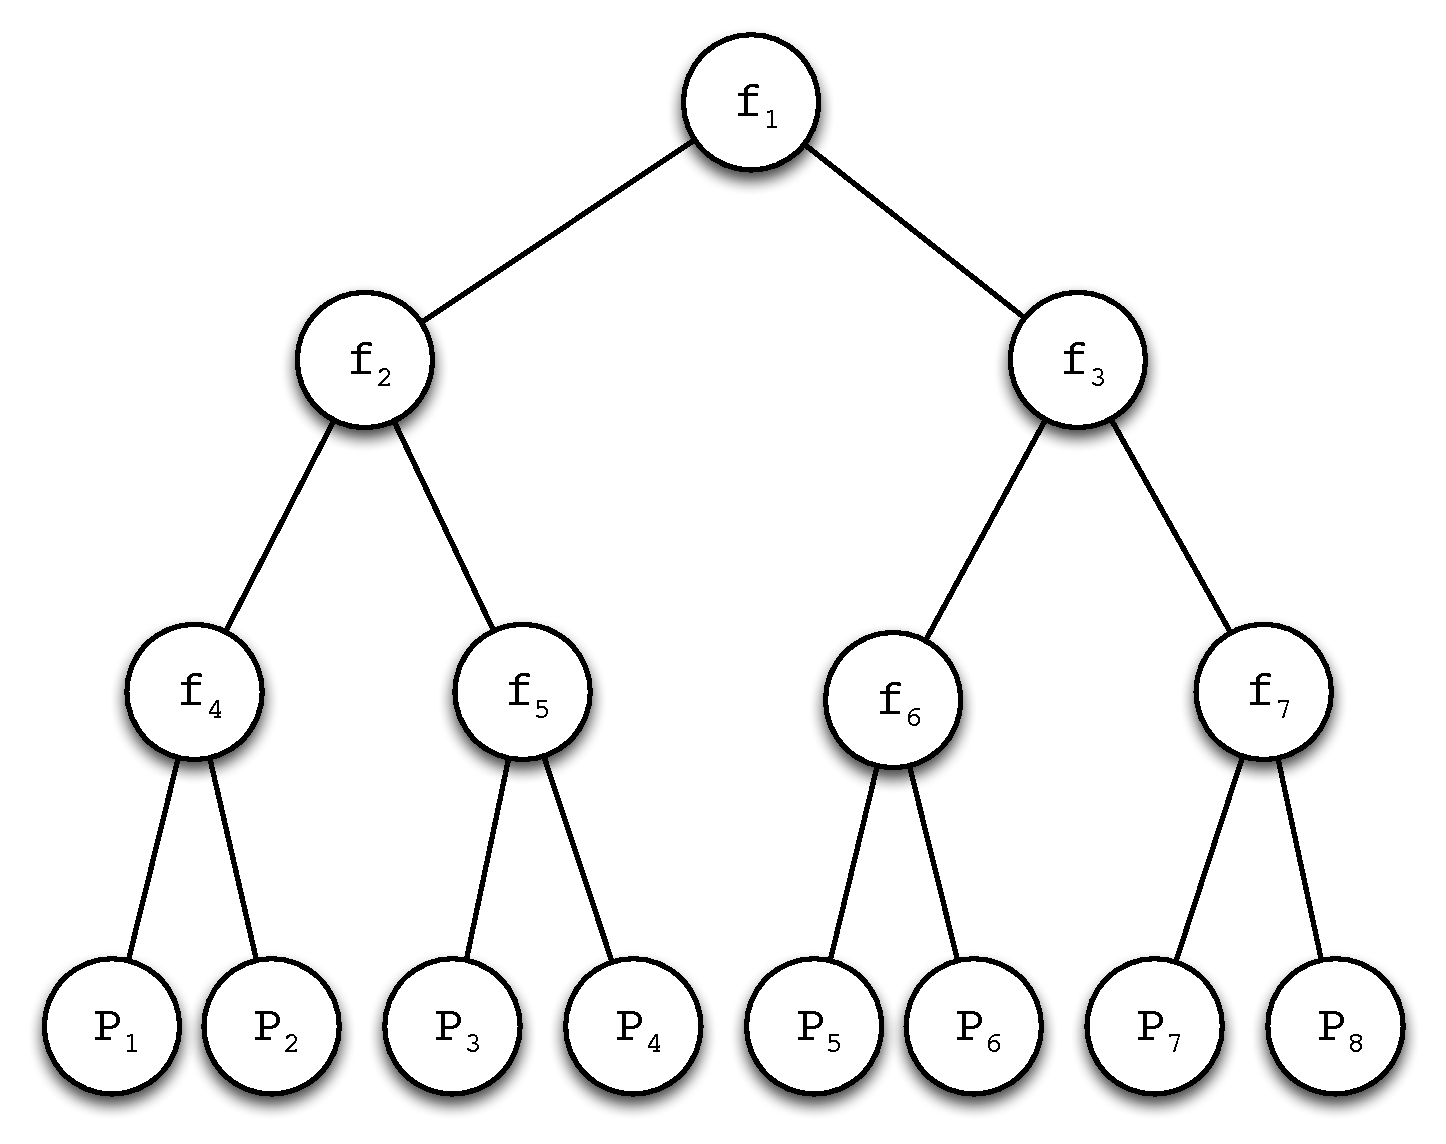
\includegraphics[width=1.0\textwidth]{figures/gp-struct.pdf}
    \caption{GP 運算樹結構示意圖} 
    \label{fig:GP-struct}
  \end{center}
\end{figure}

基因規劃藉由這樣的運算樹設計,再透過基因演算法最佳化輸入參數的選擇、不同運算節點的運算子,便可以根據資料建立出一個屬性與所求目標的關係方程式。

\subsubsection{加權基因規劃}

加權基因規劃(Weighted Genetic Programming,WGP)是由~Tsai\cite{tsai2011predicting}~所提出,基於~GP~ 方法發展而來,不同之處在於其運算樹的每個節點前都加上一個權重~$w$~,最佳化的過程除了對方程式結構和參數的選擇最佳化外,還要同時最佳化所有的權重,因此其輸出的關係方程式可能性遠大於~GP~方法,故可以處理更為複雜的問題。~WGP~的運算樹結構如圖~\ref{fig:WGP-sample}~,每個運算樹都可以組成一個數學方程式,如圖~\ref{fig:WGP-sample}~之運算樹即可組成方程式如下:

\begin{equation} w_1(w_3(\dfrac{w_7P_2}{w_8P_6}) - w_4sin(w_9\bar{C}))+w_2 \times cos(w_{12}c \times w_{11}P_1) \label{eq:WGP-sample}\end{equation} 


\begin{figure}[hbtp]
  \begin{center}
    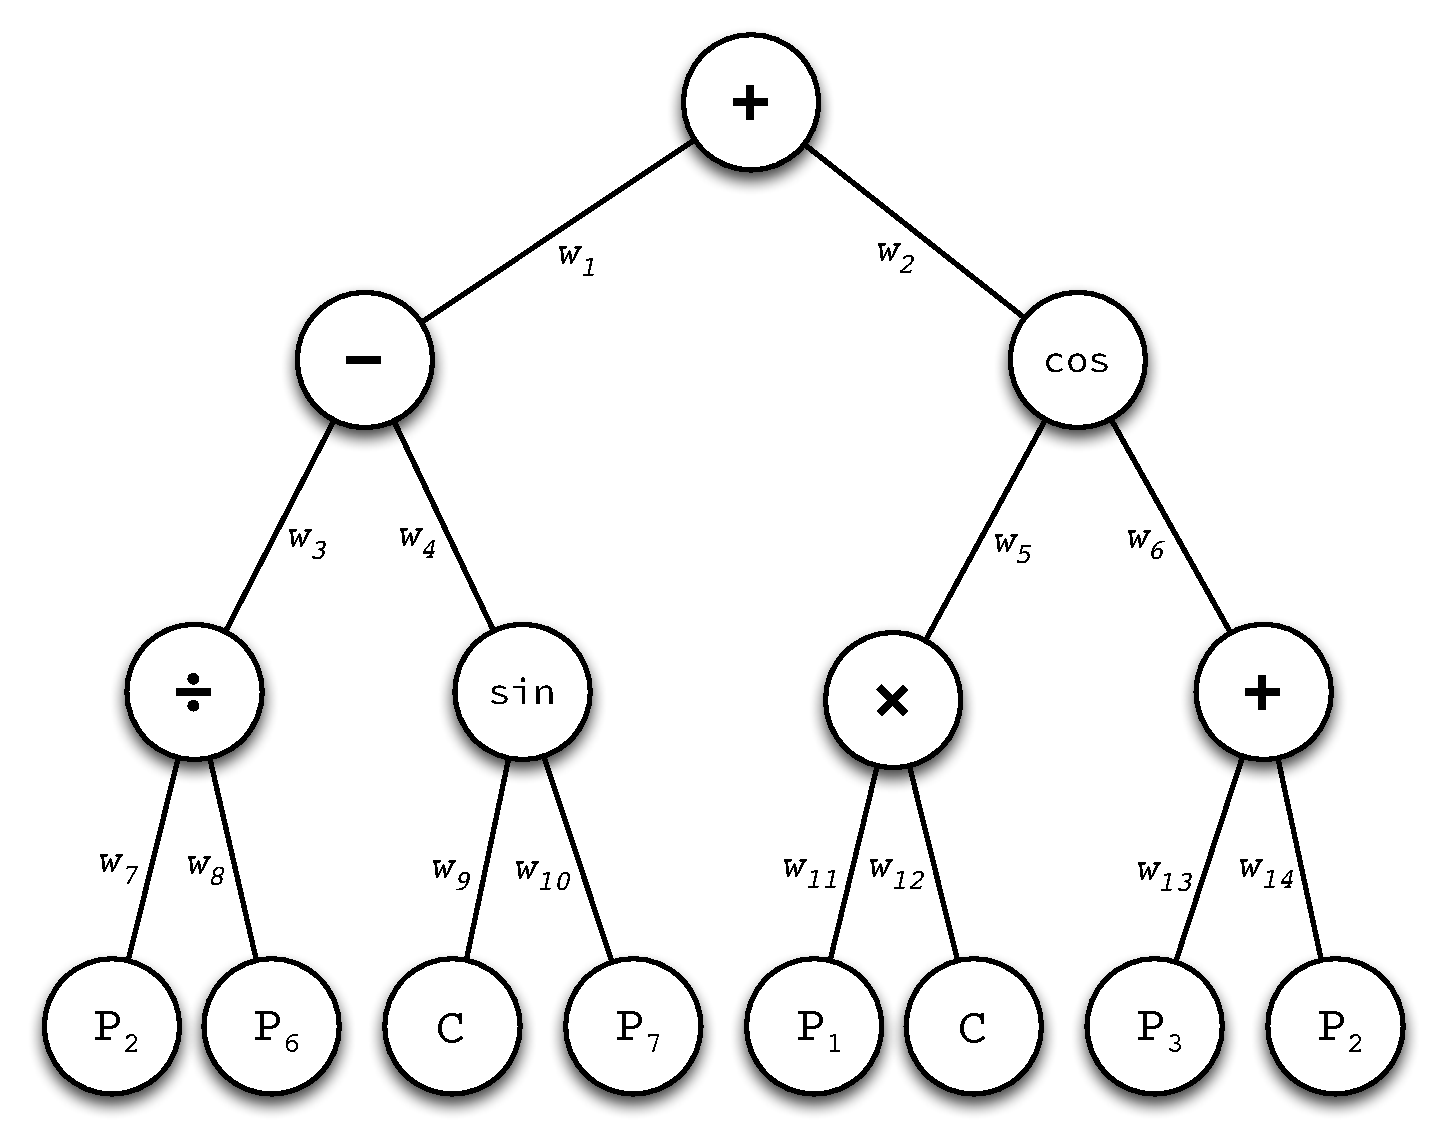
\includegraphics[width=1.0\textwidth]{figures/wgp-sample.pdf}
    \caption{WGP 運算樹結構示意圖} 
    \label{fig:WGP-sample}
  \end{center}
\end{figure}


運算樹可以分為兩種層級,運算層全部都是運算子節點,輸入層則是輸入參數的選擇,運算層每多一層,需要最佳化的節點和權重都會以等比級數成長,運算層的層數也影響到最佳化結果的方程式複雜度,而輸入層則全部都是輸入節點,每層之間的每個連結都有一個權重參數,這些權重即為~WGP~方法最大的特色,這些權重可以讓運算樹組成的方程式有無限多種,也可以用以表示不同參數的重要性,因此雖然加入權重會讓最佳化更費時間,但仍然值得加上權重。

圖~\ref{fig:wgp-unit}~是一個構成~WGP~運算樹的基本單元,和圖~\ref{fig:gp-unit}~所示的~GP~運算樹的基本單元類似,包含一個父層節點和兩個子層節點,父層的節點是運算節點~$F$,透過權重參數連接到兩個子層節點,子層節點可能是其它的基本單元或是輸入節點,而整個基本單元的輸出~$y$~為:

\begin{figure}
  \begin{center}
    \subfigure[GP]{
      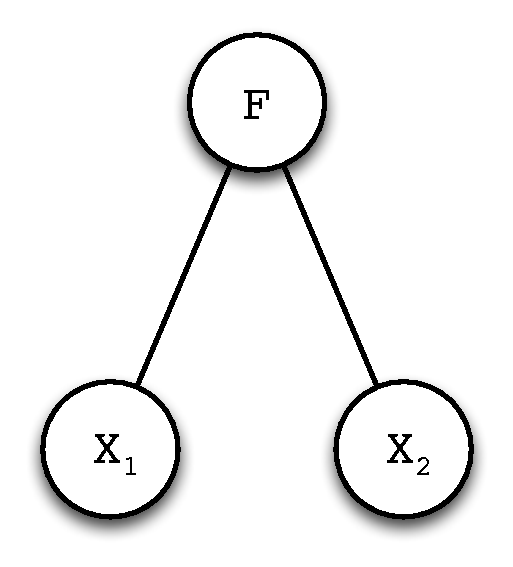
\includegraphics[width=0.4\textwidth]{figures/gp-unit.pdf}
      \label{fig:gp-unit}
    }
    ~
    \subfigure[WGP]{
      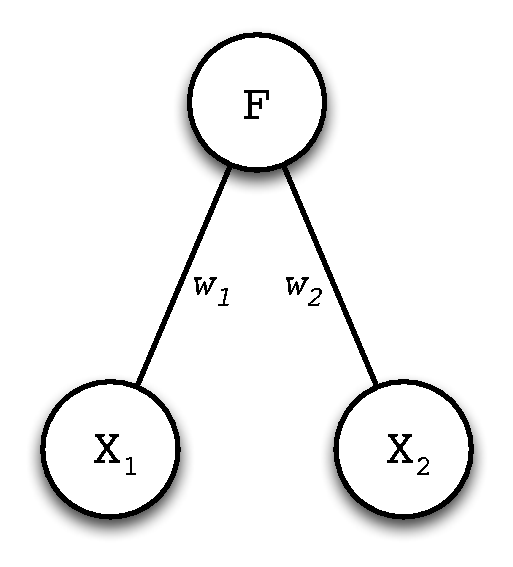
\includegraphics[width=0.4\textwidth]{figures/wgp-unit.pdf}
      \label{fig:wgp-unit}
    }
    \caption{GP 系統之單位元素}
    \label{fig:gps-units}
  \end{center}
\end{figure}

\begin{equation} y = \text{one of}\;\begin{cases}
  f_1 = w_1x_1 + w_2x_2 \\
  f_2 = w_1x_1 - w_2x_2 \\
  f_3 = w_1x_1 \times w_2x_2 \\
  f_4 = w_1x_1 \div w_2x_2 \\
  f_5 = \abs{w_1x_1}^{w_2x_2} \\
  \hphantom{f_1\;\;}\vdots \\
  f_n = \dfrac{1}{sin(w_1x_1)+cos(w_2x_2)}
\end{cases} \label{eq:WGP-y}\end{equation}

運算子~$F$~可能有數種選擇,同時配合最佳化演進得來的權重和子層節點的~$x_1$、$x_2$~,便可以計算得到這個基本單元的輸出~$y$,而子層節點的~$x_1$~和~$x_2$~有兩種可能的來源,一是此一基本單元的子層仍為運算層,則其數值要藉由計算該基本單元而來,另一種可能是子層為末端的輸入層,則~$x_1$~、~$x_2$~的值如下:

\begin{equation} x_i = \text{one of}\; \{1, P_1, P_2, P_3, \cdots P_j, \cdots P_{NI}\},\; j = 1 \sim NI \label{eq:WGP-xi}\end{equation}

其中~$NI$~為輸入參數的數量,$P_j$~為第~$j$~個輸入參數,$x_1$、$x_2$可能為輸入參數的任一個,而輸入參數也可能為常數~$1$。

運算樹的層數~$NL$~定義為有運算節點的層數,即運算層的層數,運算樹的層數大小會影響到需要最佳化的基因數量~$N_g$,其公式為:

\begin{equation} N_g = 2^{NL} - 1 + 2^{NL} + 2^{NL + 1} - 2 = 2^{NL + 2} - 3  \label{eq:WGP-N}\end{equation}


其中運算層節點的函數選擇有~$2^{NL} - 1$~個、參數層的參數選擇有~$2^{NL}$~個、以及參數的權重~$w$~有~$2^{NL + 1} - 2$~個。藉由這樣的運算樹設計,再透過~GA~最佳化輸入參數的選擇、不同運算節點的運算子和各個節點不同的權重,~WGP~方法便可以根據資料建立出一個屬性與所求目標的關係方程式。


\subsubsection{CHAID 決策樹}

CHAID(Chi-squared Automatic Interaction Detector)是由~Kass\cite{kass1980exploratory}~在~1980~所正式定名的建立決策樹的演算法,圖~\ref{fig:Decision-Tree-sample}\cite{kass1980exploratory}~即為一個典型的決策樹,決策樹是一個從根節點開始,然後根據數入屬性得資料以及不同分支的條件,移動到不同子節點,最後到達的節點的目標值即為此筆輸入屬性的預測值。CHAID~是利用卡方檢定來分析判斷輸入屬性的分割合併點,並根據不同輸入屬性對目標屬性的顯著性($p$-value)來挑選不同節點分割所依據的輸入屬性,依此建立出決策樹的分割點,可以建構出兩個以上分支的決策樹,有別於只有兩個分支的二元樹。決策樹一般是用來做分類形式的資料探勘,無法處理數值形式的迴歸,不過如果先將目標屬性區段化,則決策樹方法也可以建立出迴歸形式、用以預測數值的迴歸樹,不過由於其模型之性質,預測之目標屬性數值會分佈在特定數個數值。

\begin{figure}[hbtp]
  \begin{center}
    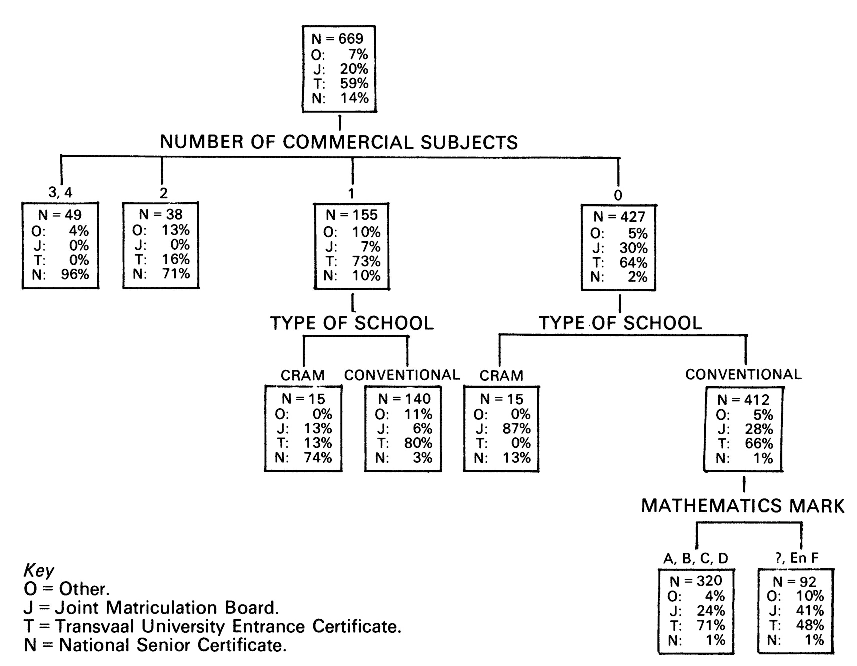
\includegraphics[width=0.8\textwidth]{figures/decision-tree.pdf}
    \caption{決策樹示意圖} 
    \label{fig:Decision-Tree-sample}
  \end{center}
\end{figure}


\subsection{分類方法}

\subsubsection{支持向量機}

支持向量機(Support Vector Machine, SVM)最早是BOSER~\cite{boser1992}等人,在~1992~年的~COLT(Computational Learning Theory)所提出,~SVM~是一個基於統計學習理論的分類方法,用來處理二元分割的問題,其原理是將原本無法線性分割的問題如圖~\ref{fig:svm}(a)\cite{verplancke2008support},將資料點轉換到一個不同維度的空間(kernel)後,假設該空間存在一超平面(hyperplane)如圖~\ref{fig:svm}(b),此一超平面可以正確的將資料分開,並將尋找此一超平面的問題轉換為一最佳化問題,求解後將此一超平面轉換回原本維度的空間即可得到二元分割邊界的方程式。而除了分類問題,Harris Drucker, et. al.,\cite{drucker1997support}~將此二元分割問題轉換為迴歸分析問題,故~SVM~也可以處理迴歸問題。

\begin{figure}[hbtp]
  \begin{center}
    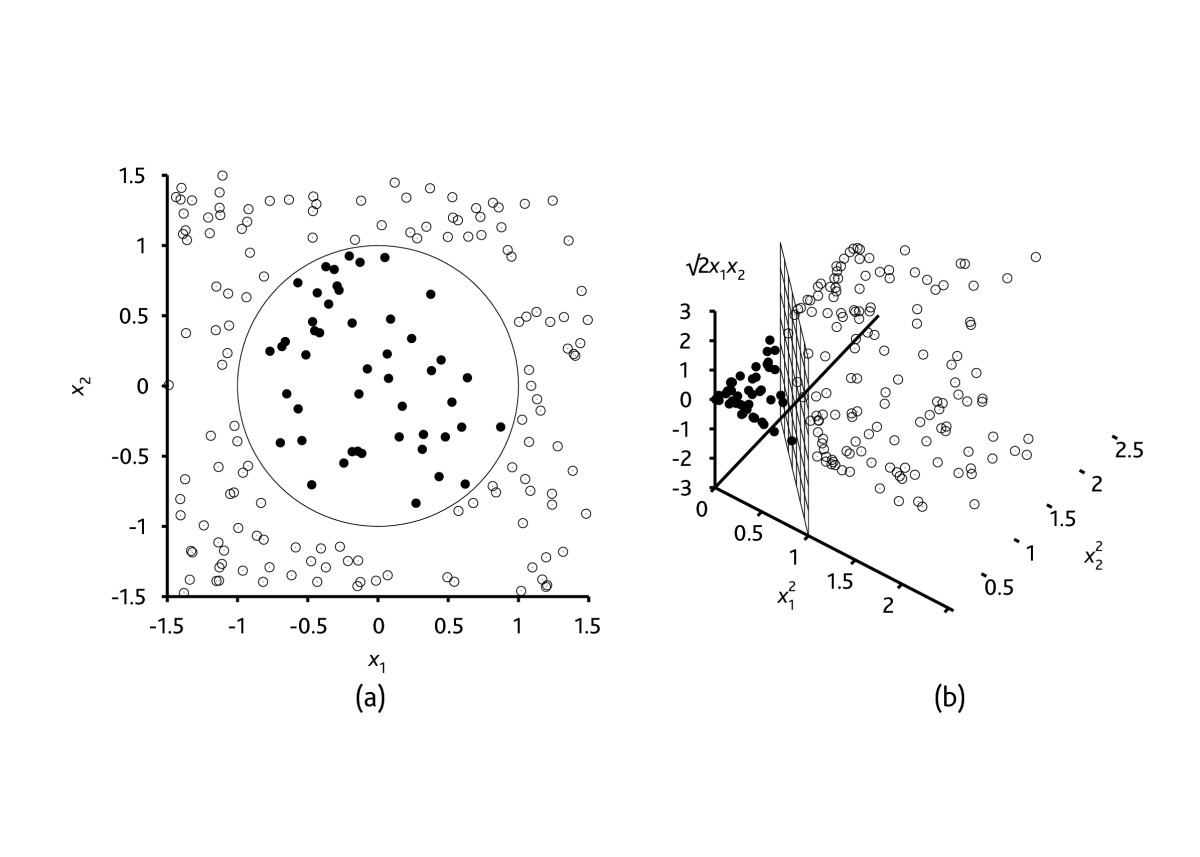
\includegraphics[width=1.0\textwidth]{figures/svm.jpg}
    \caption{SVM 示意圖}
    \label{fig:svm}
  \end{center}
\end{figure}

\subsection{分群方法}

\subsubsection{K-means}

K-means~是由~MacQueen\cite{macqueen67}~所提出,也是最常被使用的分群演算法之一,屬於機器學習方法,其主要步驟為:

\begin{enumerate}
\item 使用者決定要將資料分為幾個群集,群集數為~$K$~。
\item 將資料隨機分到~$K$~個群組,並且計算出此時分群狀態下的每個群組的中心點。
\item 將每個資料點重新分群到新的群組,新群組的選擇方法為中心離它最近的那個群組。
\item 用新的分群狀態計算出新的群組中心點。
\item 重複步驟~3~和~4~直到每個資料點的群組都穩定不再變化。
\end{enumerate}


% As proposed by MacQueen~\cite{macqueen67}, K-means is one of the most common clustering methods and has a wide application scope. Notably, it is a machine learning method; its principal steps are as follows.


\subsubsection{兩步分群}

由於各種學術、商業研究所處理的問題資料量越來越大,分群演算法所需要的運算時間也急遽的成長,為了讓分群演算在處理大量的資料時也能有良好的效能表現,而發展出兩步分群法(Two-Step Clustering),其是由~Zhang~、~Ramakrishnan~與~Livny\cite{zhang1996birch}~所提出,此一方法分為兩個主要步驟:第一步是先把資料依據其與相鄰資料的相似度來排序並分成數個小群集,相似度的計算則是使用~log-likehood~函數,接著第二步再使用階層式分群方法,將這些群集慢慢組合或拆分直到達成停止條件。其特色在於運算複雜度較其他演算法來的低,例如~K-means~演算法就需要不斷的重複運算直到所有的資料歸屬都收斂不再變化為止,因此資料量成長時也不會讓運算時間成長到無法應用的程度。

% Based on of the massive volume of basic data for school buildings in the database, this study chooses two-step clustering method. The basic concept was first proposed by Zhang, Ramakrishnan and Livny~\cite{zhang1996birch} for handling large amounts of data. This method has two major steps. The first step sequences data and pre-clusters sequences into small subclusters based on the similarity of adjacent data, thereby reducing the amount of data. The second step divides several small subclusters into the desired number of clusters using a hierarchical clustering method. The hierarchical clustering method then combines close subclusters slowly until the stop condition is met. The computing speed of this method is influenced slightly by the volume of data.

%\section{探勘結果驗證方法與指標}
\section{探勘結果指標}

%\subsection{驗證方法}

%\subsubsection{10 fold cross validation}

%\subsection{結果指標}

要驗證資料探勘所取得模型的可靠度如何,有很多的指標可以使用,分別可以從不同的角度呈現出模型的優劣,而本研究使用決定係數~$R^2$~做為判斷模型優劣的主要指標,並以其他的指標來做為輔助。

\subsubsection{敏感度分析}

敏感度分析並非用來判斷模型的優劣之用,而是用來判斷不同的輸入屬性,其資料的變異與輸出目標資料變異間的關係,定義為:

\begin{equation}  S_i = \dfrac{V(E(Y|X_i))}{V(Y)} \label{eq:sensitivy}\end{equation} 

其中~$S_i$~是第~$i$~個輸入參數的~Sensitivity Index,$V(Y)$~是目標屬性的變異數,而~$E(Y|X_i)$~是目標屬性隨著第~$i$~個輸入參數變化的期望值,$V(E(Y|X_i))$~則是此一數值之變異數,$S_i$~的值介於~0~到~1~之間,數值越高表示輸出目標對此一輸入屬性的敏感度越高,可以認為是重要度較高的輸入屬性。


\subsubsection{決定係數}

決定係數(coefficient of determination)又稱為~$R^2$~,其公式為:

\begin{equation} R^2 = 1 - \dfrac{SS_{res}}{SS_{tot}} = \dfrac{SS_{reg}}{SS_{tot}} = \dfrac{\sum{(\hat{y_i} - \tilde{y})^2}}{\sum{(y_i - \tilde{y})^2}} \label{eq:RSQ}\end{equation} 

其中 $y_i$ 是關係模型輸出屬性之值, $\hat{y_i}$ 則是該輸出屬性之實際值,$\tilde{y}$ 則是所有資料的輸出屬性實際值之平均,透過此一指標可以了解輸出屬性中有多少比例的資訊是由輸入屬性的變量所產生的,也代表著關係模型的正確性,而其值恰巧為關係係數\cite{aldrich1995correlations}~$R$(correlation coefficient)的平方,透過關係係數可以了解實際的輸出屬性數值與透過關係模型得到的推估值之間的線性關係,其值之範圍為~$0 \sim 1$,線性關係越高表示兩者之間越接近,也代表著關係模型所建立關係之正確性。

\subsubsection{平均絕對百分比誤差}

平均絕對百分比誤差(Mean Absolute Percetage Error, MAPE)~的公式如下:

\begin{equation} \text{MAPE} = \dfrac{\sum{\dfrac{\abs{y_i - \hat{y_i}}}{\hat{y_i}}}}{N} \times 100\% \label{eq:MAPE}\end{equation}

其中~$N$~是資料的總數,~$y_i$~是使用探勘得到的關係模型所求得的輸出屬性預測值,~$\hat{y_i}$~則是該屬性的實際值,此一指標代表了模型產出結果的平均誤差,可以呈現模型的準確度,數值越低代表模型品質越好。


\subsubsection{均方根誤差}

均方根誤差(Root Mean Squared Error, RMSE)定義如下:

\begin{equation} \text{RMSE} = \sqrt{\dfrac{\sum{(y_i - \hat{y_i})^2}}{N}} \label{eq:RMSE}\end{equation}

其中~$N$~是資料的總數,~$y$~是透過資料所建立的關係模型所求得的輸出屬性預測值,~$\hat{y}$~則是輸出屬性的實際值,此一指標代表了模型產出結果的平均誤差,數值越低越好,和~MAPE~相比,其差異在~MAPE~只表現了模型輸出數值的誤差平均,而~RMSE~還包含了誤差量的離散度資訊在內,~MAPE~表現相同的模型,其單筆資料誤差值分布越離散,~RMSE~的表現會越差,其可接受範圍則要根據輸出屬性的數量級和問題複雜度而定。


\subsubsection{命中率}

命中率(hit rate)是用來判斷關係模型的正確率的,判斷連續數值形式的模型正確率時,其定義為:

\begin{equation} \text{Hit Rate} = \dfrac{ \sum{I\{(1 - \alpha)y_i \le \hat{y_i} \le(1 + \alpha)y_i \}} }{N} \label{eq:hitratenum}\end{equation} 

其中~$I\{L\} \in \{0, 1\}$~,如果~$L$~為真,則~$I\{L\}$~為~1~,反之則為~0~,~$y$~是透過資料所建立的關係模型所求得的輸出屬性預測值,~$\hat{y}$~則是輸出屬性的實際值,而~$\alpha$~為命中率的容許誤差,且~$0 \le \alpha \le 1$~,如果~$\alpha = 0.1$~則表示誤差~$10\%$~內都算是有預測模型有預測命中,如果是判斷非連續數值形式的目標正確率時,例如布林值,其定義為:

\begin{equation} \text{Hit Rate} = \dfrac{ \sum{I\{y_i = \hat{y_i}\}} }{N} \label{eq:hitrate}\end{equation} 

此公式表示關係模型之目標為非連續數值形式時,要完全預測正確才會記入命中,命中率越高代表關係模型的結果越好,是一個非常直觀的模型品質指標。



\section{探勘目標分析}

由於本研究之目標在於使用各種不同形式之資料探勘方法,盡量的發掘校舍耐震資料庫中的隱含知識,因此研究的第一個步驟便是根據資料探勘方法的特性,以及校舍耐震資料庫當中所及的各種校舍資料,分析各種可能得到的知識,而根據四種主要的資料探勘知識形式及校舍耐震資料庫,分析可能可以從中探勘得到之知識如圖~\ref{fig:bigpicture}~所示。

\begin{figure}[hbtp]
  \begin{center}
    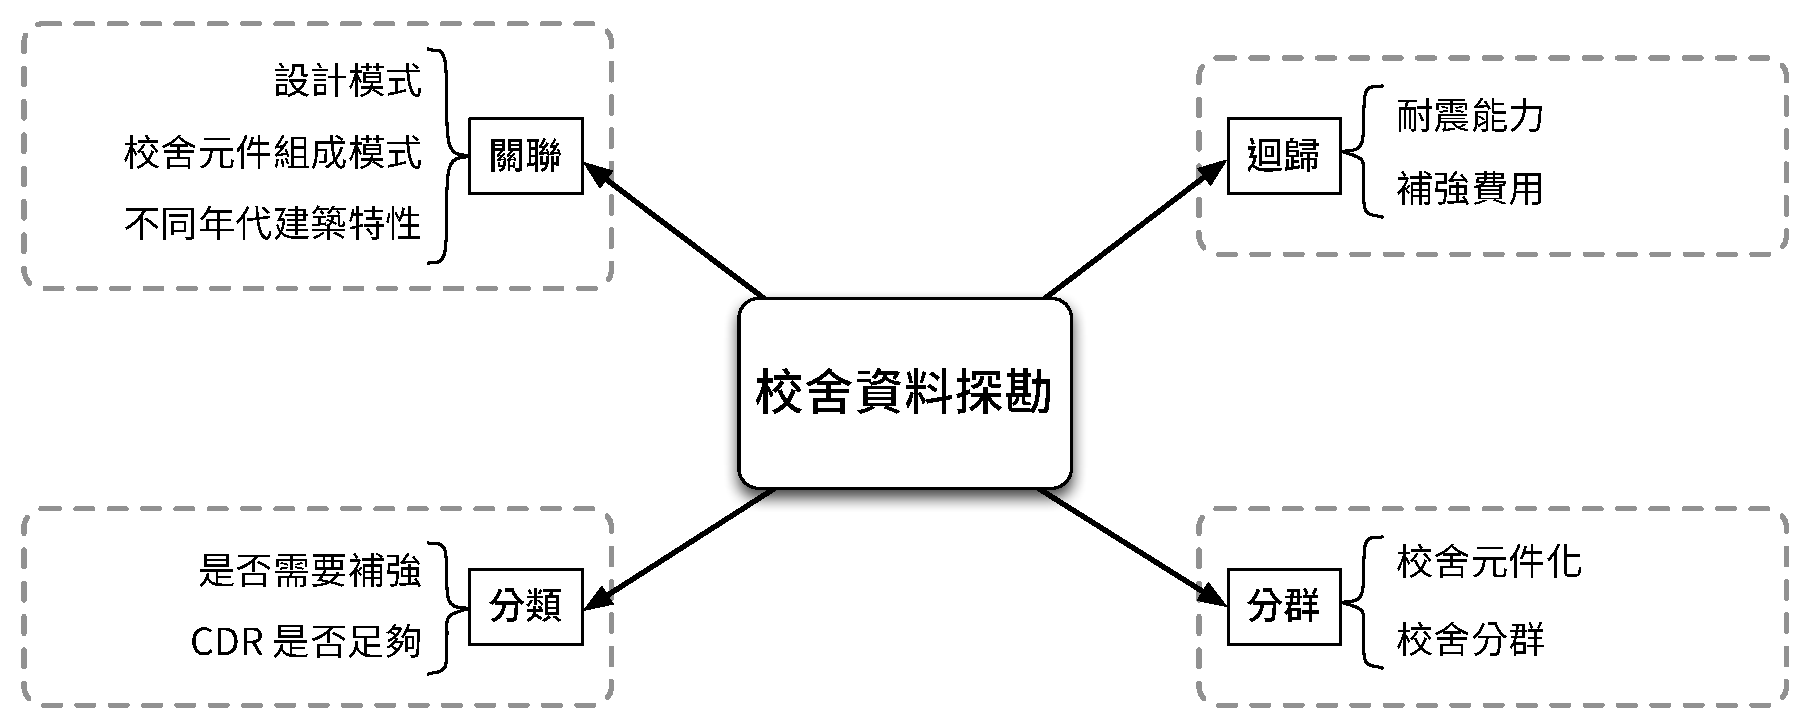
\includegraphics[width=1.0\textwidth]{figures/big-picture.pdf}
    \caption{知識挖掘規劃} 
    \label{fig:bigpicture}
  \end{center}
\end{figure}

其中,迴歸是屬於最常見的資料探勘形式,本研究所設計之迴歸形式的探勘問題包括了初步評估的~$Is$~值、詳細評估的~$CDR$~值、補強實際所花的總工程費等,在校舍耐震補強計畫中,不同階段的階段目標數值的迴歸關係模型,這些數值都是屬於連續性的數值,其數值應該與調查所得的校舍特性之間有所關聯;分類形式的知識則是以校舍是否需要補強這個詳細評估後得到的二元指標做為探勘的目標,校舍是否需要補強是整個耐震能力補強計畫當中一個非常重要的資料,如果可以透過關係模型來得知校舍是否需要補強,應該能夠讓校舍耐震能力補強計畫前半的篩選工作更有效率的執行,而在實際進行資料探勘研究後,還設計了另外一個知識探勘目標,詳細評估後的構件破壞情形與其設計參數、現況間之關係,校舍受到地震力後的構件破壞資訊可以讓,;分群形式的知識則設計有兩個,第一個是基本的校舍分群,將相近的校舍歸在同樣的群集當中,一來可以分析群集是否有顯著的特性可以探討,二來群集的資訊也可以做為其它資料探勘的參考輸入資訊。第二個分群的探勘目標是希望能夠將台灣典型校舍的結構,拆分成一些基礎的組成元件,例如教室、走廊、樓梯間等等,然後將不同的元件的各種可能模型,透過分群的方式找出,可能可以找到~10~種教室的形式、6~種走廊的配置等等,然後就可以將這些元件組合出台灣各種典型校舍,並且根據所挑選的元件,就可以得到一個可靠度足夠的校舍結構模型,並可以用來做一些模擬分析;最後則是關聯形式的知識,這類型的知識主要是可以呈現出不同的資料屬性間的趨勢與關係,因此設計上希望可以得到的知識包括了從校舍設計參數間找出校舍的主要模式,不同年代的校舍設計特色等。

而在這些研究初期所設計的資料探勘目標當中,本研究最後得到有可靠度足夠的模型為:

\begin{itemize}
  \item 校舍資訊與耐震能力之關係模型
  \item 校舍資訊與破壞構件之關係模型
  \item 校舍資訊與補強經費之關係模型
\end{itemize}

另外也使用分群方法建立出校舍的分群模型,使用~K-means~演算法將校舍分為三個群集之外,還使用~Two-Step~演算法將校舍分為兩個群集,並使用其資訊輔助耐震能力關係模型的建立,可以對模型品質有些為幫助,不過改善不明顯,且也還尚未找到明確的群集特性。而校舍元件化的分析使用初步評估所調查的校舍資料,推估出校舍的長、寬、教室柱尺寸數量、是否有窗台牆等資訊做為尋找教室元件的輸入資料,並用~K-means~分群做為主要的分析演算法,雖可以得到一些教室群集的模型,但是這些群集的特性並無法明確的判斷出來,且其屬性數值的變異性過大,不同群集但是屬性值重疊的資料比例高,難以簡單的從結構形式上分辨出不同的教室群集,因此無法更進一步的根據探勘結果將這些教室群集轉換成為教室元件,並建置出教室元件的的數值模型。而至於關聯形式的知識,目前的研究方法是做出各種假設來做探勘,例如不同年代的設計特色,就將校舍的建築年代做為關聯探勘中,屬性關聯式中一邊的屬性,關係式的另一邊則放入和校舍幾何設計相關的屬性,使用 SPSS Clemitine 的 Apriori 演算法進行分析,不過目前也還無法從這個資料庫中找到可靠的屬性關聯。



	\renewcommand\thetable{\arabic{chapter}-\arabic{table}}
%\renewcommand\thefigure{\arabic{chapter}-\arabic{figure}} 
\chapter{校舍資訊與耐震能力之關係模型}

在校舍耐震資料庫中,不同階段的調查資料有不同的校舍耐震能力指標,這些指標都是以數值形式來量化校舍建築物的耐震能力,有了此一數值後,可以快速找出有安全疑慮的校舍,根據耐震能力排序,甚至推算會需要多少預算來補強多少棟校舍等等,都可以使用此數值作為依據來達成,可以說是非常重要的校舍特性,然而要取得此一數值非常耗時耗力,如果有其他快速便宜的方法可以取得此一數值,那便可以大幅度的減少校舍耐震能力補強作業的所需要的時間與經費,因此本研究的第一個資料探勘目標,便是找出預測耐震能力索引的預測模型,得到此一預測模型後,便可以根據校舍的設計參數與現況作為輸入參數,快速的得到該校舍的耐震能力索引參考值。

初步評估階段資料的耐震能力指標是 $Is$ 值,此一數值為專業人士於現場良策、調查後,使用國家地震中心的專家根據過往的實驗數據統計分析後,所設計出的一個評估表計算而得到的,為一初步的評估值,較詳細評估所計算的耐震能力指標可靠度來的低,但仍是校舍補強計畫初期的篩選工作中非常重要的數值。詳細評估和補強設計階段的耐震能力指標則是 $CDR$ 值,$CDR$ 值是由專業人士根據校舍的設計與實際狀況建製結構模型,並進行非線性的推垮分析所得到的,此數值與建築物之設計參數為高度非線性的關係,也是最接近校舍建築物實際耐震能力的量化指標。

而除了數值量化的耐震能力指標外,本研究還將「校舍是否需要補強」($D\_isR$)這個二元指標作為耐震能力來作為校舍耐震資料庫中的第三個耐震能力指標,$Is$、$CDR$、$D\_isR$ 這三個耐震能力指標的預測模型,即為本研究所取得的第一個校舍耐震資料庫隱含知識,以下便針對不同指標的預測模型的資料探勘流程與結果詳細介紹。

\section{Is 值與校舍設計之關係模型}

校舍耐震資料庫中的初步評估資料表的耐震能力索引是為 $Is$ 值,初步評估是校舍耐震能力補強作業中,很重要的篩選過程,因為建築物的詳細評估所需要的金額極高,評估需要的時間也很長久,因此需要一個速度、價錢和可靠度都可以接受的評估方法,用比較短的時間找出耐震能力有疑慮的校舍,盡早處理。而地震中心所設計的初步評估表即為一個速度、價錢和可靠度都可以接受的評估方法,只要根據建築物的設計參數,像是樓層數、長度、深度、柱子尺寸以及校舍現況等,就可以快速的得到一個極具參考價值的耐震能力指標,而其計算的原理也與詳細評估的耐震能力指標索引 $CDR$ 值一樣,為耐震容量與耐震需求的比。找出 $Is$ 值與校舍設計參數之間的關係模型,可以進一步分析初步評估表中各種數據的重要性,並將結果回饋到此一初步評估表,將初步評估表調整的更為精簡,負責評估的人員也可以更快速的完成此意評估表格。

The proposed prediction model, based on data-mining technology, has six steps – business understanding, data understanding, data preparation, modeling, evaluation, and deployment – as recommended in the cross industry standard process for data mining (CRISP-DM) proposed by Chapman et al. (2000) (Fig. 9). The objective of this work is to construct a prediction model for the aseismic ability indices of school buildings and collect complete data. Hence, the major tasks are data preparation, modeling, and evaluation. Fig. 10 shows the procedural plan based on needs and the methods chosen. 

\subsection{資料前處理}

首先,從國震中心的校舍耐震資料庫中,將各棟校舍的 $Is$ 值與其校舍的相關資料挑出並整合在一起,第一步是過濾掉明顯不合理的錯誤資料,這些資料通常是人為的錯誤造成的,而過濾的方法則是使用國陣中心建議的過濾條件:

\begin{itemize}
\item 校舍總長或總深度超過兩百公尺
\item 有任意牆厚度超過五十公分
\item 有任意柱的長或寬超過一百公分
\item 柱間垮距超過八公尺或小於兩公尺
\end{itemize}

大約有八百筆資料符合這組基本的過濾條件,而在初步的過濾之後,前處理的第二個步驟則是減少資料屬性的維度,主成分分析(Principal component analysis)是很常使用的資料前處理方法,這個分析方法可以找出所有資料屬性中,重要度較高的屬性,它是把原始的多個資料屬性,透過向量轉換的方式,線性組合出主要的資料屬性。

Roughly 800 bits of valid data are obtained. After filtering using these conditions. Principal component analysis (PCA) is then used to reduce the dimensionality of data attributes. Notably, PCA, a very common data preparation method, can identify very important attributes among various attributes. The goal is to convert the original variables through vector transition into mutually independent variables of a linear combination. The ideal situation is that principal components obtained from linear combination retain most of the information of original variables.

校舍的分群則是基於校舍的設計模式,目標是要找出校舍建築物的幾種特定設計模式,也就是要分析校舍的幾何設計參數、柱量、牆量等等,經過不斷的測試及調整,最後找出了五個主要成分屬性:

\begin{itemize}
\item 走廊柱資訊
\item 教室柱資訊
\item 強設計資訊
\item 牆量資訊
\item 柱量資訊
\end{itemize}


Clustering analysis of school buildings is based on the design patterns of school buildings; the goal is to find several design patterns. Hence, the attributes for analysis are the geometric information of school buildings, such as dimensions and quantity of walls and columns, and width and height of school buildings. Other attributes, such as year of construction and locale, may not be incorporated into PCA analysis. After continuous testing and adjustment, five major attributes are obtained and the importance of constitutional fields is considered as the basis for naming. The five attributes are as follows: corridor column information; classroom column design information; wall design information; data for number of walls; and, data for number of classroom columns.



在前面的處理完成後,還使用分群分析將校舍分群,以幫助後續的 $Is$ 值關係模型的建立,分群的目標是將校舍依照不同的設計模式特性區分開來,將相近設計的校舍放在同一群集,分群的依據是主成分分析法所找出的五種主要校舍設計相關屬性,圖十一是使用 SPSS Clemitine 進行此一分群分析時的節點設計圖,分別使用的 K-means 和 Two-Step 兩種分群演算法,其參數設定如下:

After data preparation, clustering analysis is utilized to find hidden design patterns of school buildings. This study uses the K-means and two-step clustering methods. Fig. 11 shows the node deployment for clustering using the SPSS Clementine (2007) software. The parameter choices for the two methods are as follows.

\subsubsection{K-means}

此一分群方法最重要的設定參數是初始的群集數 $k$,雖然有許多研究都在研究如何找出最佳的 $k$ 值,但是目前仍沒有一個方法可以宣稱它找到 $k$ 值是最佳的,唯有對該領域的專業了解以及詳細的測試才能得到最佳的 $k$ 值,在本分析案例中,K-means 分群的停止條件是設定為 20 次迭代,如果 $k$ 太大,那會造成分群結果無法在 20 次迭代內收斂,如果 $k$ 小於 6,則分群的結果就可以在 20 次迭代內完整的收斂,每筆資料都會故底定在所屬的群集內,不在變動,最後挑選的 $k$ 值是 5,而根據此意參數的分群結果可以找出三個主要的校舍群集,分別的比例是 28\%、56\% 和 16\%。

The most important parameter with this clustering method is the initial group, k. Although many researchers have developed methods for choosing the initial K value, no method can confirm that it has found the best K value. The best K can be found only based on researcher understanding and problem testing. In this study, K-means clustering is set to stop after 20 iterations. If the K value is too large and cannot be completely converged after 20 operations, some data points will continue to change the clusters to which they belong. When the K value is reduced to <6, Clustering models can be completely converged after 20 iterations, become stable, and no longer change cluster label of all data bit. The K value chosen is 5, and three major clusters are obtained. The remaining two clusters have few data and are considered outliers. The distribution of three major clusters are 28\%, 56\%, and 16\%.

\subsubsection{Two-Step}

Two-Step 分群有兩個優點,一是複雜度不高,運算時間與資料數量間之關係為線性關係,第二個優點就是不需要由人工決定分群的群數,演算法即可自己根據資料狀況決定,操作人員只需給予上下限,在本分析中,上下限的設定為最少兩個群集,最多八個群集,而最後的分析結果是所有的資料都被分到兩個群集中,分別佔了 54\% 和 45\%。

This clustering method has two features. The first is enhanced scalability. The algorithm has low complexity. Computing time does not grow nonlinearly as data volume increases. The other feature is that it can determine the number of clusters, unlike K-means clustering, which requires manual designation of parameters. However, this work can designate the upper and lower limits for the number of clusters. This work sets the limit to 2–8 clusters based on experience with K-means clustering. Consequently, all data are divided into two clusters, accounting for 54\% and 45\% of all data.






此資料探勘分析還用了十群交叉驗證來驗證結果的可靠度,因此資料前處理的最後一個步驟就是將整理好的資料隨機分為十組。

This work uses 10-fold cross validation to validate the prediction model. After preparation, data are grouped by first dividing data randomly and equally into 10 clusters. One cluster is then chosen as a dataset for validation and the remaining nine clusters are combined into one training dataset.

\subsection{資料探勘}

完成資料前處理,將校舍的群集分好之後,才開始建立 $Is$ 值與校舍設計參數的關係模型,本分析使用了廣義線性模型、線性回歸和類神經網路三種分析方法,每種方法都有三種分析資料群,分別為先經過 K-means 分群的資料、先經過 Two-step 分群的資料及沒有先經過分群的資料。圖 12 為使用 SPSS Clemitine 分析時的節點設計圖。以下分別對三種分析方法的參數設定作說明。

The prediction model is built only after clustering is completed. This work uses a GLM, simple regression, and ANNs to build the prediction model based on three groups of data – not clustered in advance, clustered by K-means, and clustered by the two-step method in advance. In total, nine prediction models are generated. Fig. 12 shows the node configuration within SPSS Clementine. Below are the parameters chosen for the three methods. 

\subsubsection{Generalized linear model}

廣義線性模型是假設在輸入參數和預測目邊之間有一個可以用連結函數表達的關係,這個連結函數可能是指數函數、對數函數、Logistic 函數等,經由一些測試資料的測試,我們選擇使用對數函數作為連結函數,並且根據實際的資料分布選擇了常態分布作為輸入參數的分布函數,而關係模型的分布也選擇常態分布,因其表現教其他分布形式較好。

The GLM assumes a relationship between input variables and a predictor; this relationship can be built by a link function such as identity function, log function, logit function, or power function. After available link functions testing on some data, the prediction model performs best when using log function as the link function; hence, this work chose the log function. The distribution function of the predictor is based on the actual distribution of data. This work chose the normal distribution, which is close to the real data distribution. The prediction model constructed using the normal distribution performed better than those with other distribution types.

\subsubsection{Simple regression}

線性回歸是選擇使用最小平方根法來建立校舍建築物的設計參數與其耐震能力 $Is$ 之間的關係,這也是最常使用的回歸方法之一。

Simple regression in this work uses the least square method by adopting the building design parameters as independent variables $X$ and the aseismic ability of buildings as dependant variables $Y$. The linear equation between regressed design parameters and aseismic indices serve as the model for predicting aseismic ability $Y$ based on building design parameters $X$.

\subsubsection{Artificial neural networks}

類神經網路需要決定的參數包括隱藏層的數量、每層的神經元數量、學習率、停止條件等,除了直接設定神經網路的參數,還有一些方法可以使用,例如 dynamic、multiple 或是 prune method 可以用來調整並找出最佳的神經網路大小和結構,dynamic method 是從一個小型的神經網路開始(兩個隱藏層、每層兩個神經元),慢慢成長,並且比較成長前後的神經網路效能與結果,Multiple method 則是同時產生各種不同的神經網路,並且一起訓練到達停止條件,然後在從中挑選出表現最好的一個,而 Prune Method 則是從一個大的類神經網路開始,慢慢的把重要度低的神經元節點拿掉。本分析最後挑選的是 Exhaustive Prune Method,是 Prune Method 的一種修改形式,對於節點的篩選要求較高,是所有方法中最花時間的,但是通常也可以找到最好的結果。其他的類神經網路設定參數為:初始的神經網路為兩層隱藏層,其中一層有 30 個神經元、一層有 20 個神經元,停止條件為 250 個訓練循環,在這個設定下,Exhaustive Prune Method 是表現最好的方法。

Generally, ANNs must decide on such parameters as number of hidden layers, number of neurons in each layer, learning rate, and stop condition. Aside from directly setting these parameters, methods such as dynamic, multiple, and Prune methods are available for adjusting and finding the optimal size and structure of the neural network. The dynamic method starts with a small neural network (two hidden layers with two neurons for each layer), expands network size gradually, and decides on the further expansion based on model performance before and after expansion. The multiple methods constructs multiple neural networks simultaneously, trains all neural networks to reach the ``stop condition,'' and then selects the group with the best performance. In contrast with the dynamic method, which slowly builds a large neural network from a small one, the Prune method first builds a large network and then removes neurons with low importance based on training. This work chooses the exhaustive Prune method, a special application of the Prune method. The initial neural network has two hidden layers, one with 30 neurons and the other with 20 neurons. The stop condition is set to 250 training cycles. Under this limit, the prediction model built by the exhaustive Prune method performs best.


\subsection{驗證}

驗證有兩個主要的目的,一是確保資料探勘找到的關係模型的可靠度,而不會找到只適用於該組訓練資料集的關係模型,第二個目的是可以用來作為比較不同分析方法的指標數據,本分析使用的驗證方式是十群交叉驗證,這個方法將所有的資料等分成十份,每次挑選九組出來作為訓練資料集,留下一組作為驗證資料集,如此可以得到十組模型以及其可靠度的指標,求此十組指標平均值即可得到代表此關係模型的可靠度代表值,而本分析所選擇的指標有三個,線性關係、絕對平均誤差(Mean Absolute Prediction Error, MAPE)以及 hit rate。

Validation work has two purposes. The first is to ensure model reliability instead of to generate only good performance during data training. The second is to serve as a benchmark for comparing the performance of different prediction models. This work uses 10-fold cross validation to assess and compare the performance of prediction models. This method divides a fixed amount of data into 10 groups, conducts 10 rounds of model building and validation, chooses a different group of data for testing, trains the model with remaining nine groups of data, and uses test group data to validate model accuracy. After validation for 10 times, the accuracy of the 10 models is obtained and their average is taken as the accuracy of this algorithm. This study uses linear correlation, mean absolute prediction error (MAPE), and hit rate as the indices for comparing the prediction model performance.

\subsection{結果}

此資料探勘分析會產生九個校舍耐震能力與校舍建築設計資訊間的關係模型,包括直接使用GLM、線性回歸和類神經網路的三組,混合使用 K-means 或是 Two-Step 分群的六組,要比較其優劣我們使用了線性關係 $R$ 、 MAPE 和 hit rate 三個指標,並配合十群交叉驗證,其中線性關係 $R$ 之公式為:

This work constructed nine prediction models; three are directly generated by the GLM, simple regression, and ANNs. The mixed model of K-means and two-step clustering generated three prediction models. Hence, nine models were obtained and 10-fold cross validation is used to compare the performance of the three reference indices – R2, MAPE, and hit rate. Notably, R2, the linear correlation is

\begin{equation} R = \dfrac{\sum{(\hat{y_i} - \tilde{y})^2}}{\sum{(y_i - \tilde{y})^2}} \label{eq:RSQ}\end{equation} 

其中 $y_i$ 是校舍的實際耐震能力指標 $Is$ 值, $\hat{y_i}$ 則是透過此關係模型的到的推估耐震能力指標值,$\tilde{y}$ 則是所有資料的 $Is$ 值之平均,透過此一公式即可得到實際的 $Is$ 值與透過關係模型得到的推估值之間的線性關係,線性關係越高表示兩者之間越接近,也代表著關係模型的正確性。MAPE 的公式為:

where yi is the aseismic CDR of school buildings obtained using nonlinear analysis of the database, yi is the CDR obtained from the prediction model, and y~ is the average aseismic CDR of school 651 buildings obtained using nonlinear analysis. The correlation between aseismic CDR of school buildings obtained via the prediction model and nonlinear analysis can be determined based on linear correlation. A high CDR indicates a strong correlation and many opportunities to make correct predictions. The MAPE is derived as

\begin{equation} MAPE = \dfrac{\sum{\dfrac{y_i - \hat{y_i}}{y_i}}}{N} \label{eq:MAPE}\end{equation} 

其中 $N$ 是資料總數,MAPE 的是用來表示關係模型誤差之數值,由於關係模型不可能完全沒有誤差,即使有非常高的線性關係也是會有誤差,因此會使用 MAPE 作為判斷其誤差程度的參考。 hit rate 的定義是:

where N is the number of samples. The MAPE is used to judge the  degree of error of prediction models as the prediction result always has errors, although the prediction mode has an adequately high R2. The hit rate is derived as 
hit rate

\begin{equation} hit\ rate = \dfrac{ \sum{I\{(1 - \alpha)y_i \le \hat{y_i} \le (1 + \alpha)y_i \}} }{N} \label{eq:hitrate}\end{equation} 

其中~$0 \le \alpha \le 1$~,且~$I\{L\} = 1$~。hit rate~是用來判斷關係模型的正確率的。在本分析中,我們設定了兩個~$\alpha$~值作為~hit rate~指標用,分別是~0.1~和~0.2~,表~\ref{tab:is_result}~列出了這九個關係模型使用這三個指標配合十群交叉驗證所得到的數值,表現最好的關係模型是先使用~K-means~分群再使用~GLM~所建立的,第二好的則是先使用~Two-step~分群再使用~GLM~所建立的,圖~13~是先使用~K-means~分群再使用~GLM~所建立模型的實際~$Is$~值與使用模型得到的~$\hat{Is}$~值的比較圖,資料點的回歸取現的斜率非常接近~1~,可以看得出來兩者之間的相關度非常高。如果單看模型的線性關係表現,類神經網路的表現比~GLM~ 和線性回歸都要來的好,這也可以驗證校舍的耐震能力與其設計參數之機善一個非線性的關係,而雖然~GLM~整體的排名較~ANN~來的好,但是~hit rate~卻是~ANN~表現的比較好,但是看到~MAPE~又會發現~ANN~的~MAPE~較大,因此我們建議在~$Is$~值的關係模型的挑選,可以依據應用的需求來決定,如果需要較高準確率的時候,建議使用~ANN~,如果是需要降低整體的誤差,則建議使用~GLM~。如果先使用分群方法將校舍資料根據設計參數分出不同群集後,再對不同群集分別探勘其耐震能力與設計參數的關係模型,結果會比沒有先分群要來的好一些,探討其原因,是因為典型校舍已經是校舍建築物的一個子集合,而此子集合的特性已經非常接近,因此再進行分群也不會有顯著的改善。


\begin{table}[hbtp]
  \begin{center}
    \caption{Cross-validation result of the prediction model}
    \label{tab:is_result}
    \scriptsize
    \begin{tabular}{l c c c c c c c c c}
      \hline
       & K-means & Two-step & ANNs & K-means    & Two-step   & Regression & K-means & Two-Step & GLM \\
       &   ANNs  &   ANNs   &      & Regression & Regression &            &   GLM   &   GLM    & \\ 
      \hline
	   R              & 80.21\% & 81.78\% & 80.76\% & 72.16\% & 72.16\% & 72.15\% & 87.41\% & 87.11\% & 87.05\% \\
       MAPE           & 28.69\% & 26.64\% & 26.51\% & 46.06\% & 46.05\% & 46.05\% & 24.68\% & 24.70\% & 24.71\% \\
       hit\_rate(0.2) & 53.12\% & 54.29\% & 54.31\% & 40.16\% & 40.17\% & 40.21\% & 48.82\% & 48.64\% & 48.52\% \\
       hit\_rate(0.1) & 27.71\% & 28.72\% & 28.75\% & 21.13\% & 20.98\% & 21.09\% & 25.05\% & 25.16\% & 25.16\% \\
      \hline
       Rank & 6 & 4 & 3 & 9 & 7 & 8 & 1 & 2 & 4 \\
      \hline
      \end{tabular}
  \end{center}
\end{table}

When 0<a<1 and I{L} = 1, hit rate is utilized to determine the percentage of data predicted correctly by the prediction model, that is, prediction model accuracy. In this work, the hit rate is ranked by setting a equal to 0.1 and 0.2, which are utilized as two assessment indices that average and rank the performance of accuracy. Table 1 lists the assessment indices of the nine prediction models. The prediction model that performs best is that built using the GLM with K-means clustering. The second best prediction model is that built via the GLM with two-step clustering. Fig. 13 compares the actual CDR and CDR obtained using the K-means and GLM prediction models. The slope of the regression curve equation approaches 1, indicating a strong correlation between school building design data and aseismic ability of building. However, the scattered distribution of actual data points corresponds to a high R2 and high MAPE. After a thorough comparison of the nonlinear analysis by ANNs, the GLM, and linear analysis by simple regression, the ANNs perform better than the GLM and linear analysis by simple regression all aspects, confirming that the design parameters of school buildings have a nonlinear relationship with aseismic ability, which conforms to the fact that the aseismic CDR in this work is obtained using nonlinear analysis. Although the GLM ranks high in comprehensive assessment, its hitate is worse than that of ANNs; ANNs also have a higher MAPE. Hence, it is possible to determine which prediction method is suitable based on actual needs when predicting the aseismic ability of school buildings. We recommend using ANNs for accurate prediction of the aseismic abilities of school buildings; however, the drawback in using ANNs is that the prediction model generated is a black box. We recommend using the GLM to minimize total error. When building prediction models by clustering first and then comparing the performance of the three assessment methods, the prediction model built with clustered data performs slightly better than those built directly, indicating that traditional school buildings are already a subcluster of various architectural patterns. One feature of subclusters is their weak correlation with the aseismic ability of school buildings. Hence, information added to the cluster will not markedly improve prediction model quality.

由於校舍補強預算和時間有限,因此其執行的優先順序就會依照評估得到的耐震能力作為參考排序,因此本分析還用此實際的應用作為另一個評量關係模型優劣的指標,此指標將所有的校舍依照其~$Is$~值排序後,照順序等分成~10~群,另外在用關係模型得到的~$\hat{Is}$~排序,一樣照順序等分為 10 群,接著比較每筆校舍所分配到的群集,如果實際所屬的群集編號和關係模型得到的群集編號一樣,則誤差(error)為~0,如果差了一號,則誤差為~1,差了兩號則誤差為~2,表~\ref{tab:is_seq_result}~即為九組關係模型的排序誤差結果。可以發現表現最好的一組仍然為先使用~K-means~分群再用~GLM~ 探勘所得到的關係模型,其誤差小於 1 的資料比例為 70.8\%,誤差小於~2~的資料比例則有~88.9\%~。

The budgets and priorities for reinforcing school buildings are based on the aseismic abilities of school buildings. This work analyzed the sequencing result of aseismic ability of school buildings by sequencing school buildings based on CDR values, dividing them into 10 equal zones, and comparing the zone number of actual and predicted values. Table 2 shows the zoning result. When Error = 0, the predicted and actual values have the same zone number; when Error = 1, predicted and actual values are in adjacent zones; when Error = 2, predicted and actual values are separated by one zone. The prediction model built by the GLM with K-means clustering performs best. The zoning error of this prediction model <1 is 70.8\%, and the zoning error <2 is 88.9\%, indicating that the prediction model already has sufficient accuracy when sequencing is used.

\begin{table}[hbtp]
  \begin{center}
    \caption{Sequencing analysis of prediction of aseismic ability}
    \label{tab:is_seq_result}
    \scriptsize
    \begin{tabular}{l c c c c c c c c c}
      \hline
       Error & K-means & Two-step & ANNs & K-means    & Two-step   & Regression & K-means & Two-Step & GLM \\
             &   ANNs  &   ANNs   &      & Regression & Regression &            &   GLM   &   GLM    & \\ 
      \hline
	   0  & 32.8\% & 35.0\% & 33.9\% & 33.4\% & 34.1\% & 33.3\% & 35.6\% & 34.9\% & 35.0\% \\
	   1  & 36.0\% & 35.2\% & 36.5\% & 35.4\% & 34.2\% & 35.5\% & 35.2\% & 35.9\% & 35.7\% \\
	   2  & 17.5\% & 15.2\% & 16.2\% & 16.6\% & 17.1\% & 16.4\% & 18.1\% & 17.3\% & 17.5\% \\
	   >2 & 13.7\% & 14.6\% & 13.5\% & 14.6\% & 14.7\% & 14.8\% & 11.1\% & 11.9\% & 11.8\% \\
      \hline
      Rank & 5 & 5 & 4 & 7 & 9 & 8 & 1 & 2 & 2 \\
      \hline
      \end{tabular}
  \end{center}
\end{table}

\section{CDR 值與校舍設計之關係模型}

校舍耐震資料庫中,詳細評估表的耐震能力索引 $CDR$ 值是用來評估校舍是否需要補強、甚至是拆除的最重要依據,此數值的取得非常耗時耗力,且與校舍結構材料、設計與現況等參數之間為高度非線性的關係,如果能夠取的此一關係模型,對於校舍耐震能力補強計畫的進行,可以有很大的幫助。

\subsection{資料前處理}

人工輸入的資料很容易發生單位錯誤或是格式不正確的資料,而資料的品質對於資料探勘的結果優劣影響很大,因此需要在資料前處理時把這些問題都處理過,資料前處理的最主要目標是讓處理過的資料能夠很確實的反映出分析問題所要尋找的資料特性,使用的方法包括資料過濾、屬性過濾、新屬性的生成等,首先,本分析中第一個前處理工作就是資料過濾,要把有問題的資料,不合理的資料都過濾掉,過濾的條件則是依照國震中心所建議的典型校舍特性的過濾條件:

Manually inputting data may result in incorrect units or formats because controlling data quality in the real world is difficult. Hence, it is necessary to pre-process data before building the relational model. Quality, as an important part of soft computing and data analysis, has considerable influence on subsequent analytic results or even on the reliability of the generated model. Apart from the actual data, the researcher also refers to expert advice from NCREE for data pre-processing. The main target of data pre-processing is to ensure the accuracy and adjustment of the data in a format that clearly reflects the target of analysis. Pre-processing includes data screening, property screening, and new property synthesis. Data screening is divided into two stages. The first stage is the rationality screening of the data. Pre-existing mistakes are unavoidable because the data in the School Building Database were entered manually; the obligation is to identify such mistakes. Most of the school buildings were I-type shaped buildings; a very common design. . With regard to the properties of these school buildings, the NCREE (2005) suggests the following screening conditions:

\begin{itemize}
\item 校舍深度介於六到二十公尺之間
\item 校舍垮距介於二到八公尺之間
\item 每間教室至少有一個垮、兩個柱
\item 
\item 校舍的破壞地表加速度是長向較小
\end{itemize}


\begin{itemize}
\item Total depth of the school building should exceed 20 meters or is less than 6 meters
\item The span exceeds 8 meters or is less than 2 meters
\item The number of spans for a single classroom is less than 1
\item The number of columns in the classroom is low
\item The collapse ground acceleration of the major direction is greater than that of the minor direction
\end{itemize}

由於並不是所有的校舍都有進行過詳細評估,因此第二個步驟就是要挑選出同時有基本設計資料以及詳細評估的 $CDR$ 值的資料,接著,由於校舍資料庫中的原始資料,每棟校舍都有上百個資料屬性,因此接著要對屬性進行篩選與合併,與國震中心之專家討論過後,挑選過濾掉大部分的屬性,但是仍然有約三十多個屬性,因此為了能夠繼續減少資料屬性,本分析接著還繼續對這些資料的屬性進行分類,根據其屬性分布挑選出一組典型校舍子集來分析,這個挑選出來的子集其特性為:

In the second stage, choosing school buildings with both basic design parameters and minimum destruction ground acceleration is necessary because not all school buildings have detailed information.According to the raw data in the seismicassessment database for school buildings, each data set contains hundreds of properties. Based on our judgment with expert which are non-structural and low importance, and synthesize some properties with similarity. There are still more than 30 properties left after this reduction process. This study further classifies school building records into subsets based on similarities in property values, and chooses one subset with major population as the data set for further studying. After the classification of school buildings, we try to do further reduction and finally determine a set of key properties which is optimal to represent the seismic characteristics of individual school buildings. The choice is based on data distribution, and a subset that correctly represents I-shaped school buildings. The features of this subset adopted in this study are listed below:

\begin{itemize}
\item 沒有走廊柱
\item 只有一種教室柱
\item 校舍沒有 RC 牆
\item 沒有四面圍束磚牆
\item 沒有三面圍束磚牆
\end{itemize}

\begin{itemize}
\item No corridor columns
\item Only use one type of classroom column
\item School buildings have no RC walls
\item School buildings have no brick walls with four-side confinement
\item School buildings have no brick walls with three-side confinement
\end{itemize}

最後前處理完成的資料總共有~107~筆。並且依照專家建議挑選出~12~個屬性,分別為表~1~中的 $P_1$ 到 $P_{12}$,其中~$P_{11}$,$S_{DS}$~ 是校舍的設計地表加速度,~$P_{12}$,$S_{D1}$~則是一秒週期的設計譜加速度,都是分析校舍耐震能力時非常重要的參數,另外也根據專家的建議,使用現有的資料組合出兩個新的屬性,分別是 $P_{13}$ 和 $P_{14}$,分別代表了校舍的教室數量和校舍建築物的垮距。

After finalizing the data for the first and second stages, 107 datasets conform to the above condition. Twelve properties are then chosen for the screened data with reference to expert advice, displayed as P1 to P12 in Table 1. In addition to the screening based on existing properties, this study synthesizes two new properties, P13 and P14. They represent the number of classrooms and number of spans for a single classroom, respectively, based on expert advice and existing data. In P11, SDS stands for design spectral response accelerations at short-periods, and in P12, SD1 stands for design spectral response accelerations at 1 sec. These two parameters represent the magnitude of the seismic force at the building’s location, and are very important parameters for analyzing the aseismic ability of buildings by non-linear analysis.

前處理的最後一個步驟是資料的正規化,因為不同屬性的物理意義不一樣,其數值的數量級差異也很大,如果有一個重要參數其數量級很小,那就會增加探勘的難度,因此為了減少數量級差異造成的影響力落差,要先把參數經過正規化處理,正規化的方法很多,可以把屬性的數值調整至~0~到~1~的區間,也可以用標準差和平均值來作調整,其最重要的目標是要保留原始數值的分布,本分析則是對~$P_2$、$P_3$、$P_7$、$P_9$~和~$P_{10}$~除以~1000,讓這些屬性的數值和其他屬性的數值比較接近。

The last step of data preprocessing is normalization. The purpose of normalization is to balance the impacts of the parameters in different scales. If an input parameter has small values of mean and standard deviation, but is of high importance and if the result is also sensitive to this parameter, then it is necessary to use data normalization to prevent its influence from being overshadowed by other larger scale parameters. Normalization methods include converting the data into the range of 0 to 1, using the maximum and minimum values, and converting data to the standard deviation of its mean. The normalization principle adopted in this paper is to retain the original values as far as possible, so only a few parameters with large values, such as P2, P3, P7, P9 and P10, are divided by 1000 to make their scale comparable to other parameters.

完成以上所有的前處理工作後,可以得到~107~筆校舍資料,每筆資料有~14~個屬性,本分析就是針對這個資料集作分析。

After the three pre-processing steps, 107 datasets and 14 properties were obtained. The subsequent analysis was based on this dataset.

\subsection{資料探勘}

\subsubsection{Genetic Programming}

雖然校舍耐震能力的資料中,最能代表校舍耐震能力的數值是~$CDR$~值,但是由於其組成成分中的~$AD$~值的數值是根據建築物所在地而決定的,和校舍設計、建築方式有關係的參數則是~$AC$。因此本分析使用資料探勘所尋找的知識為校舍設計參數與校舍破壞地表加速度~$AC$~間的關係模型,首先是使用~GP~方法來進行資料探勘,使用~GP~分析的結果可以作為了解模型複雜度的參考。運算樹的層數影響了所建構模型的複雜度,越多層可以建構出越複雜的模型,然而卻可能會造成無法收斂、運算時間太長或是太過複雜的模型等問題,本分析先使用不同的運算樹層數來進行測試和調整,最後根據運算所需時間和模型的結果表現,選擇了~4~和~5~層兩個運算樹層數來進行後續的資料探勘,在本分析中使用了多組不同的參數設定進行測試與探勘分析,最後的結果是使用~200~組基因、~5000~次的演化,並且交配率是~0.8~、突變率是~0.1~,而交配函數使用的是~Scattered~函數,突變函數使用的是~Adaptive Feasible~函數,兩者都是非常通用的函數,可以處理各種不同面向的問題。表二是此分析中~GP~演算法的資料探勘結果的~RMSE~(均方根誤差)值。

An AC model was built for this study to represent the relationship between the basic design parameters of school buildings, and minimum destruction ground acceleration. GP was the first model to be used, and based on a preset number of tiers for different operation trees; it can result in relational equations with different degrees of complexity. In this case, several operation trees with different number of tiers were tested, and it was found that the most suitable number is either four or five. Having a low number of tiers leads to reduced complexity of the relation model and hence, poor performance. Conversely, large numbers result in many difficulties, such as convergence problems, time-consuming progressive computation, and a very complicated relationship model. The optimum setting is 200 populations of 5000 progressive iterations, a crossover rate of 0.8, and a mutation rate of 0.1. The crossover function used in this paper is the scattered function. The mutation function is the adaptive feasible function. Both these functions can be applied to solve many different problems. The scattered function diversifies the child layer after crossover. The adaptive feasible function is suitable for the constrained minimization problem. This setting was chosen after the analysis was conducted 30 times. Table 2 shows the root mean square (RMSE) of the model generated.

RMSE~是本分析案例中最主要用來判斷模型品質的索引,定義如下:

RMSE is the index used in the current study to judge the quality of models, and is defined as the equation below:

\begin{equation} RMSE = \sqrt{\dfrac{\sum{(y_i - \hat{y_i})^2}}{N}} \label{eq:RMSE}\end{equation}

其中~$N$~是資料的數量,~$y$~是使用探勘得到的關係方程式所求得的建築物耐震能力~$AC$~值,~$\hat{y}$~則是詳細評估的非線性分析所得到的建築物~$AC$~值,建築物的破壞地表加速度分布在~0.04~至~0.5~之間,NCREE~專家則建議~RMSE~值需要低於~0.04~,此模型才夠有能力用來鑑別校舍的耐震能力優劣與否,表二中的控制組則是使用~SPSS Clemitine~的類神經網路所建立的模型,類神經網路的設定為使用~Exhaustive Prune method~來發展神經網路,初始神經網路為兩層隱藏層,分別有~30~個和~20~個神經元,訓練~250~個週期,結果的~RMSE~是~0.041~,非常接近目標的~0.04~,本分析使用了~WGP~來建立校舍的~$AC$~值與其設計參數間的關係模型,結果的模型其品質和使用類神經網路所建立的模型非常接近,然而類神經網路所建立的模型其複雜度太高,且其機制為一黑盒子,而~WGP~方法產生的模型就只是一個代表方程式的運算樹,可以非常快速的將結果拿到各種不同環境或平台中應用,

where n is the number of datasets, $y$ is the estimated value obtained from the equation, and $\hat{y}$ is the actual unit-less deviation index value (the smaller the better). The ground acceleration of the minimum destruction obtained from the nonlinear analysis was distributed between 0.04 and 0.5, and therefore, the relationship model has a sufficient recognition rate. Experts from NCREE recommend that the RMSE must be below 0.04. The control group is the relationship model obtained from the artificial neural network. In applying the relationship model constructed by SPSS Clementine and choosing the Exhaustive Prune method to adjust the number of tiers and nodes, the initial neural network has two hidden tiers with 30 and 20 neurons, respectively. The neurons have been trained for 250 iterations, and those with a low degree of importance are removed during the training period based on the situation. The resulting RMSE is 0.041, which is close to the target of 0.04. In this paper we use WGP to create an aseismic ability prediction model for real school buildings. The quality of our model is similar to models built using Artificial Neural Networks. However, Artificial Neural Network based models are complicated; their mechanism is in a black box. The WGP model, on the other hand, is just an equation of the building’s design parameters and its aseismic ability. Thus, it can easily be ported to other platforms and programming languages for use in many applications. The optimum model obtained from the GP pattern is represented by the relationship equation below. Function nodes in a tree topology, displayed in Figure 8, uses several symbols and text to represent the F of that node.

``+'' 代表 $f = x_1 + x_2$; \\ \indent
``-'' 代表 $f = x_1 - x_2$; \\ \indent
``×'' 代表 $f = x_1 \times x_2$; \\ \indent
``÷'' 代表 $f = x_1 / x_2$; \\ \indent
``pow'' 代表次方函數 $f = {x_1} ^ {x_2}$

結果使用~GP~方法所建立的關係模型其表現並不好,~RMSE~只能達到~0.056~,而根據圖九可以發現,其實使用~GP~方法並沒有正確的建立~$AC$~和校舍設計參數間的關係模型,因為他只使用了三個輸入參數,而且其方程式也非常的線性,可以推斷出此一個關係模型的複雜度很高,而~GP~方法並不能正確的找出這個關係。

The performance of this model is not ideal because the RMSE can only reach 0.056. Based on Figure 9, the relationship model generated did not correctly build the relationship between the design parameters of school buildings, and ground acceleration of the minimum destruction. As only three input parameters were used, it resulted in the minimum equation as the linear equation. This can be attributed to the fact that this seismic ability model for school buildings has high complexity, and the application of GP pattern alone cannot obtain the relationship between them. The WGP pattern was then used to build the relationship equation between the design parameters of school buildings, and ground acceleration of the minimum destruction because it could be used for relationships that are more complex than with the GP pattern.

\begin{equation} AC = \dfrac{P_3}{P_{11}} + P_3 P_{12} - P_3 {P_{12}}^3  \label{eq:GP_AC}\end{equation}

\subsubsection{Weighted Genetic Programming}

WGP~是本分析第二個使用的方法,和~GP~一樣選擇了五層的運算樹,其他的基因演算的參數也都和~GP~分析中使用的一樣,~200~組基因演化~5000~代,交配率是~0.8~,突變率是~0.1~,而唯一不一樣的參數則是權重~$w$~的範圍,設定為~+10~到~-10~間,在此設定下分析~30~次,從中挑出表現最好的一組關係模型,其~RMSE~直在表二中,圖10是此關係模型的運算樹結構,其符號定義與~GP~方法運算樹使用的一樣,唯一不同的是黑色實心點,代表的是~$f = w_1x_1$~,此關係模型的方程式如下:

WGP was used as the second model, which also chose five tiers of the operation tree. The optimum setting of GA is the same with GP: 200 populations of 5000 progressive iterations, a crossover rate of 0.8, and a mutation rate of 0.1. The best group was chosen after the analysis was conducted 30 times. Contrary to GP, the weight was set from +10 to -10 within the weighted (w) range. Table 2 shows the RMSE of the model generated, and the four-tier optimum equation is shown as Equation (9). The tree topology generated is displayed in Figure 10, and uses the same symbol as the GP tree topology to represent the same operator. The other symbol that was used is a black solid dot, which represents f=w1x1.

\begin{equation} AC = {({165 P_{10}}^{8.86 P_6} {P_4}^{4.86} + \dfrac{22.5 P_8 + 39.5 P_{10}}{P_{10}} )}^{-98.6 P_4{P_8}^{-1.3} - 133 P_{10} - 0.05 {P_7}^{1.38 P_{10}} }  \label{eq:WGP_AC}\end{equation}

表二列出了~WGP~方法所建立的校舍設計參數與其最所破壞地表加速度~$AC$~間關係模型的~RMSE~值,其值為~0.039~,比使用類神經網路所建立的關係模型表現還要好,圖12是此模型的推估值與實際直的比較圖,可以看得出來比使用~GP~所建立的模型要來的好。

Table 2 shows the RMSE of the optimum relationship equations generated from the two patterns. The RMSE reached 0.039, which is better than the performance of the model built by the artificial neural networks in the contrast group. Figure 12 displays the comparison between the estimated, and the actual values of the model. By comparing the results, the model constructed by the WGP pattern is superior to the model constructed by the GP pattern.

本研究還分析了此關係模型所使用到的輸入參數,表三列出了此關係模型所有使用到的輸入參數,~$S_{DS}$~和~$S_{D1}$~並沒有被使用到,因其兩者都是和耐震需求相關的參數,而本分析的主要目標是校舍的地震承受能力,也就是耐震能力相關的部份,而此結果也正可以符合預期,而其餘所有的參數都有被使用到,也可以代表前處理所選擇到的參數都有其重要性。

The parameters entered are analyzed based on the equation obtained from WGP, and Table 3 shows the input parameters obtained from the optimum relationship equations. SDS and SD1 were not used, as both are relevant to the demand of the CDR. For this study, the target is to estimate the Capacity (Aseismic Ability Index), which is irrelevant to Demand. Hence, this result conforms to the expectations. As all of the remaining input parameters were used, this indicates that the parameters chosen at the data processing stage are important.

\subsubsection{Capacity Index Formulation Tuning}

CDR~是詳細評估所得到的,校舍建築物的耐震能力指標,是校舍結構所能承受的地震力和規範所規定,校舍所在位置所需要能承受的地震力的比值,~CDR~大於~1~表示其耐震能力足夠,如果~CDR~等於~1~則表示耐震能力與需求相等,然而~$Is$~值的數量級和~CDR~不一樣,~$Is$~是百分系統,~100~表示耐震能力與需求相等,不過~$Is$~內其實還有一個調整參數~$I$~為~1.25~,而此時如果~$CDR$~是~1~則~$Is$~是~80~,這個關係可以用來將~$Is$~值轉為~$C_E$~值,其物理意義和~$AC$~相同。

Similar with the CDR obtained from the detailed estimation, the aseismic capacity index of school buildings is the demand ratio of the aseismic capacity, excluding the ability unit and measure. CDR is directly compared to the ground acceleration, and IS is the estimated force ratio. If CDR is greater than 1, then the building has sufficient aseismic capacity. If CDR is 1, the building has an aseismic capacity equal to the demand. However, it should be noted that IS is a hundred-mark system, and 100 indicates that the capacity is equal to the demand. IS also needs to consider the usage coefficient I, of buildings. When IS equals 1.25, CDR is 1 and IS is 80. This relationship can be described by a formula that converts IS into CE, which has the same meaning as the ground acceleration of the minimum destruction.

\begin{equation} C_E = f(Is) = \dfrac{Is \times Demand \times I}{80}  \label{eq:CE}\end{equation}

$I$~是確保~$C_E$~值能趨於保守用的係數,在~NCREE~的設計中,校舍的~$I$~定為常數,為~1.25~,~$C_E$~即為最小破壞地表加速度,不過其可靠度較詳細評估所得到的數值低,因此本研究下一個分析目標即為修正初步評估的公式,為~$C_E$~加上一個調整因子~$T$~,可以讓其結果更接近詳細評估所得到的最小破壞地表加速度。

I is the usage coefficient that intends to keep the seismic design at the conservative side, and prevents miscalculations caused by the insufficient estimation of the earthquake destruction. For this study, I is set to a constant of 1.25 for school buildings. Demand is set to different recommended values based on the positions of the school buildings. It represents the minimum ground acceleration that the buildings can withstand in the area. The School Building Database contains the demand data that was determined by engineers, based on the actual situations. This study adds T to CE as a revised formula, such that it is closer to the minimum destruction ground acceleration AC, of school buildings obtained from nonlinear analysis.

\begin{equation} AC = C_E + T  \label{eq:AC}\end{equation}

基於之前的結果,本分析只使用~WGP~來分析,基因演算的參數也和之前一樣,~4~或~5~層的運算樹,~200~初始基因,~5000~個演化週期,交配率為~0.8~,突變率為~0.1~,訓練出~30~組模型後,從中挑選出最好的模型,結果~$T$~的模型為一個~4~層的運算樹,如圖~11。

Based on the analysis above, this study only uses the WGP pattern to build the model, and this can be applied to complicated situations. Parameters chosen are: the operation tree has four to five tiers, 200 populations of 5000 progressive iterations, crossover rate of 0.8, mutation rate of 0.1, and choosing the best group after the analysis was conducted 30 times. The optimum T generated from the four-tier operation tree is shown in the equation below, and the tree topology is displayed in Figure 11.

\begin{equation} AC = C_E + 0.54 \dfrac{P_3}{P_2} - 24.86 \dfrac{ {P_6}^{0.36P_3} }{ {P_5}^{2.6P_9} } - ( 37.84 \dfrac{P_5}{0.67P_2 + 5.52P_7} )^{\left[ (-0.67 P_{12})^{1.23P_7/P_{13}} \right]} \label{eq:WGP_AC_IS}\end{equation}


\subsection{結果}

表二顯示了~NCREE~初步評估~$Is$~值轉換成詳細評估~$AC$~的等價數值~$C_E$~與校舍實際進行詳細評估所得到的最小破壞地表加速度~$AC$~相比的~RMSE~,為值~0.067~,距離目標的~0.04~還有一段距離,圖~13~是~$C_E$~與~$AC$~的比較圖,可以發現其趨勢相近,加上修正因子~$T$~之後,~RMSE~降低為~0.045~,圖~13~顯示了~$C_E + T$~和~$AC$~的比較,可以發現其趨勢更為接近,因此可以確定修正因子確實可以將初步評估的結果停整的更好。

Table 2 shows the RMSE after the revision. The RMSE of the IS formula used by NCREE in the preliminary appraisal is 0.067. Although there is still a gap between the target of 0.04 and this value, the emphasis is on the degree of relationship between them, and the main target is to screen out the school buildings with degrees of higher risk. Figure 13 shows the comparison between the CE converted from IS of NCREE, and the destructive ground acceleration obtained through linear analysis. Even though the data have the correct directional tendency, the model obtained from the GP method is better because of higher deviation, and a linear relationship. Subsequent to adding T to the revised formula, RMSE is reduced to 0.045. Figure 13 shows the comparison, and it can be seen that the directional tendency is quite close, thus reducing the deviation. A good revision effect is observed, making the screening result of the preliminary appraisal more accurate.

表三呈現了此分析中所有使用到的輸入參數,四層運算樹和五層運算數分別使用到的參數分開表示,其中:樓層數($P_1$)、總樓地板面積($P_{10}$)和單間教室的垮數($P_{13}$)並沒有被使用到,其中前兩個參數對於校舍結構的耐震能力來說非常重要,在~$Is$~的推估過程中已經有使用到,而本分析的修正因子並沒有使用到可以顯示~NCREE~的初步評估已經很完整正確的表現出這兩個參數所造成的影響,而單間教室垮數的資訊則可能在初步評估的過程中已經將該資訊表現在評估公式內了,因此修正因子~$T$~的公式內並不包含它,不過此參數在前一個分析中依然有使用到,因此仍然有其重要性。

Table 3 shows the input parameters used by the equation obtained from the WGP method, and by the optimum relationship equations with four to five tiers. The number of floors (P1), total floorage (P10), and number of spans in a single classroom (P13) were not used because the number of floors and total floorage, which are highly important, were already used in the IS formula. Hence, IS has been correctly included in the two properties above, and the number of spans in a single classroom can be inferred as hidden in the formula. Hence, T in the revised formula will not use this input parameter. However, the input parameter is still used to directly construct the relationship equation in the previous case, and has a certain degree of importance.



In order to estimate the aseismic ability of a building, we need to obtained detailed information about its geometric dimensions, the properties of materials used, etc. and we may need to perform sampling and other experiments to obtain certain information e.g. the properties of materials used. Based on this information, a structural model of the building has to be constructed and then non-linear pushover analysis is used to perform estimation. This process is time-consuming, and technicians are required. It usually takes about one months to estimate the aseismic ability of a building.

在校舍資訊與耐震能力之關係模型之分析中,本研究提出了基於~WGP~方法所建立的關係模型,只要透過校舍結構的基本參數就可以推估校舍的耐震能力,其前處理的工作可以分為兩個部分,第一個部分是資料的過濾與挑選,其而過濾與挑選的條件是基於專家的建議,第二個部分是找出不同資料屬性的重要性,第一步是先將和校舍結構非關以及明確不重要的資料屬性剃除,接著藉由將校舍分成不同子集,並逐步減少資料屬性,最後選出了~14~個資料屬性,然後基於這個子集進行資料探勘分析,相較於原來上百個資料屬性,本分析達到了一個非常高效的資料壓縮,減少了非常多的資料雜訊。

In this study, we adopted the WGP method to construct a relation model, which uses the basic design parameters of school buildings to estimate their aseismic ability. The pre-processing efforts carried out for the proposed prediction model can be divided into two parts. The first part is a data filter for selecting out data sets which are reasonable as typical school buildings. The selection conditions of this data filter is proposed based on judgment with expertise in structural engineering. The second part is the determination of the key properties used in the proposed model. We first eliminate some properties which are non-structural and low importance, and synthesize some properties with similarity. We further classifies school building records into subsets based on similarities in property values, and chooses one subset with major population as the data set for further studying. Based on this subset, we try to do further reduction and finally determine 14 properties which are optimal to represent the seismic characteristics of individual school buildings. In comparison with hundreds of properties in the original data, a very high reduction ratio is reached.

~WGP~最大的特色就是其產生的模型結果是使用數學方程式的形式來呈現,因此可以很簡單的就將產出的模型拿到不同的系統或平台中應用,除~WGP~外,本分析也使用了~GP~來進行分析,經過比較可以發現~WGP~方法所建立的模型的表現要比~GP~方法的好很多,可以顯示其對於複雜問題的處理能力是更為優秀的,而其~RMSE~也可以低於~0.04~,比類神經網路的表現還優秀,透過預測值與實際直的比較圖,也可以發現其趨勢都是正相關,驗證了使用挑選出的~14~個參數和~WGP~方法所建立的關係模型是可以在校舍補強工作上使用的。

Same as GP, a key characteristic of WGP is the resulting model is in the form of mathematic equation, which is very easy and convenient to be applied in engineering practice, and thus is more practical than other soft computing methods. This study also applies GP on the same set of school building data for predicting the building’s collapse ground acceleration. Compared to the prediction results by using GP, the accuracy of WGP model is much better. This case shows WGP can handle problems with more complexities than GP. Regarding the application of WGP method, this study performs 5000 iterations of revolutions for test models with operation tree from two to five levels respectively, and determines the optimized values of model parameters, such as the crossover rate and mutation rate, for this application case through repeated tests. The RMSE of the resulting model achieves less than 0.04. This accuracy in prediction is comparable with the model using Artificial Neural Networks (ANNs). In addition, the graph compared the actual values with predict values shows the distribution trend of the data points are consistent with the expected direction. The result verification indicates the proposed WGP-based model successfully establishes the relation between the 14 input properties and the output property, building’s collapse ground acceleration. In practice, the proposed model can be applied directly and efficiently for preliminary assessment of school buildings for seismic capacities.



In addition to directly inferring the aseismic capacity of school buildings from the design parameters, the current study revised the aseismic capacity index formula of school buildings designed by NCREE using GPS. The formula was to provide greater accuracy with a smaller deviation. This model can help decision makers with issues that are related to the aseismic capacity of school buildings, as well as estimating the disaster loss, during a disaster in a timely manner. These applications require that the estimation of the aseismic capacity of many school buildings be generated rapidly, and this would be impossible if traditional non-linear structural analysis were applied.

\section{D\_isR 值與校舍設計之關係模型}

「校舍是否需要補強」此一指標其數值之基礎即為詳細評估的耐震能力指標 $CDR$ 值,$CDR$ 值超過 1 表示其耐震能力尚符合安全規範,反之,則是有安全疑慮,需要進一步補強或是拆除。而 $D\_isR$ 則是標記各校設耐震能力是否足夠的二元指標,也是教育部的校舍耐震能力補強計畫中,前期篩選工作的最主要目標。找到這個指標與校舍設計、現況等參數的關係模型,與 $Is$ 值和 $CDR$ 值關係模型一樣,此一關係模型對於校舍耐震能力補強計畫中,初期的篩選工作可以有很大的助益,也可以輔助決策者編定預算、快速的根據狀況決定不同計畫年度補強的規模等。

\subsection{資料前處理}
\subsection{資料探勘}
\subsection{結果}


	\renewcommand\thetable{\arabic{chapter}-\arabic{table}}
%\renewcommand\thefigure{\arabic{chapter}-\arabic{figure}} 
\chapter{校舍資訊與破壞構件之關係模型}
\label{cha:crack} 

校舍耐震評估最準確的階段為進行詳細評估作業,但進行校舍詳細評估須歷經非常多之流程如圖~\ref{fig:FLOW}~,花費很多時間,如能有一輔助工具在校舍詳細評估前期即可粗估校舍之可能破壞構件與其破壞模式,將有助於技師與專業人是進行作業時先有初步結果之掌握,瞭解校舍的弱點以及可能的破壞形式,便能夠針對這些重點多加檢視,提升整體之評估水準,因此本研究也對於此一知識進行探勘分析。

在校舍耐震資料庫中所記錄的校舍破壞元件的資訊,是記錄在\nameref*{appendix-de}中之資訊,記錄了校舍在詳細評估的側推分析下,首先破壞的結構元件,包括了樑、柱、窗台柱、磚牆、RC~牆等構件,並且記錄了破壞樓層以及破壞形式,如剪力破壞、撓曲破壞等。而本分析之目標則是要尋找此一資料集與校舍的基礎設計參數間之關係,由於要分析的破壞構件種類較多,難以用單一個模型建構出其多重關係,因此本分析將此問題拆成數個較為單純的問題,單獨針對不同構件是否破壞進行資料探勘分析,並將主要的正向破壞挑出作為探勘目標,分別進行了五組資料探勘分析。


\section{資料前處理}

本分析之前處理分為三個階段,分別為資料合理性篩選、資料屬性的篩選以及新屬性之合成,首先,資料合理性篩選一樣依照~NCREE~所建議之規則篩選,資料屬性之挑選則分為兩個步驟,第一個步驟是根據資料之分佈挑選資料子集合,藉由此一步驟可以適當的排除少數結構形式的校舍,並同時縮減資料屬性的數量,降低資料複雜度,挑選的條件為:

\begin{itemize}
\item 鋼筋混凝土建築
\item 單邊走廊且廊外無柱
\item 無地下室
\end{itemize}

同時由於選出資料的此三屬性的數值均相同,因此三個條件相關的屬性便在此過程被過剔除;接著則是進一步挑選資料屬性,降低資料的複雜度,本分析依照不同屬性與校舍耐震能力間之關係作為挑選依據,將完全無關以及有重複性質之屬性剔除,再將重要性較高之屬性挑選出,並保持屬性數量不要過多,根據測試結果合成出部分新屬性,最後挑選之屬性如下:

\begin{multicols}{2}
\begin{itemize}
\item 校舍長度
\item 校舍深度
\item 樓層數
\item 地上層樓地板總面積
\item 一樓教室柱根數
\item 一樓走廊外柱斷面積和
\item 475~年設計地表加速度
\item 校舍垮距
\item 用途係數
\item X~向~1F~三面圍束磚牆斷面積
\item 有無三面圍束磚牆
\item 有無四面圍束磚牆
\item 有無磚牆
\item 同時有三面和四面圍束磚牆
\item 有無~RC~牆
\item[]
\end{itemize}
\end{multicols}

其中校舍跨距資料是根據現有資料推估的估計值,因此一資料並未在校舍補強工作的流程當中有紀錄,合成之公式為:

\begin{equation} \dfrac{\text{校舍長度}}{^{\text{一樓教室柱根數}}/_2 - 1} \label{eq:span}\end{equation} 

本分析其餘所挑選之資料屬性介紹與選擇說明如下:

\begin{description}
  \item[校舍長度、深度]
  中小學校舍中之典型校舍其建築形式較為固定且普遍存有耐震能力較弱之現象,因此本分析推測在這些典型校舍中,某些特定尺寸之校舍應與其極限強度下會破壞之構件與其破壞模式存有一定之相關性。因此本分析將此二屬性納入屬性集做為本探勘模型之輸入屬性。
  \item[樓層數]
  加入此屬性,其構想為假設這些校舍中應該有集中幾層樓之建築與其極限強度下會破壞之構件與其破壞模式存有一定之相關性。因此本分析將此屬性納入屬性集做為本探勘模型之輸入屬性。希望藉由其中隱藏之關聯性達到目標之預測。
  \item[地上層樓地板總面積]
  校舍之樓地板面積亦屬於建築形式之一環,因此可視為該校舍之特有形式,本分析假設在典型校舍中,特定樓地板面積大小有其普遍對應之耐震能力,抑或是某些尺寸之樓地板面積可能存有較高的機率需要接受補強。
  \item[一樓教室柱根數]
  教室柱之根數間接可表現校舍樓地板面積之大小或規模,且其為結構之乘載元件因此本分析將之視為影響工程經費之因素之一,經將此屬性納入探勘模型中測試後,也確實發現此屬性對預測之正確率有一定之提升。
  \item[一樓走廊外柱斷面積和]
  台灣中小學校舍其建築形式較為固定,教室柱之多寡或其尺寸亦可視為建築形式中之一環,因此本分析推測在這些校舍中,教室柱應該存有某些特定總斷面積大小之校舍其耐震能力較差,因此本分析將此屬性納入屬性集做為本探勘模型之輸入屬性。
  \item[475~年設計地表加速度]
  由校舍所在位於查出其工址短週期設計水平譜加速度之~0.4~倍($0.4S_{DS}$),同時也代表耐震需求,是判斷耐震能力是否足夠非常重要的屬性。
  \item[用途係數]
  此一屬性為紀錄該校舍是否作為緊急避難使用,以決定其值為~1.25~或~1.5~,為反映其因重要性所需之安全係數。如該校舍當初規劃為緊急避難使用,那其當初設計強度就會比較高,用途係數除了可以反應校舍耐震能力之需求外,校舍最初在設計建造時,校舍對於耐震能力需求的差異,應該也會直接反映在校舍實際的耐震能力上,因此將之加入本屬性集內。
  \item[X~向一樓三面圍束磚牆總斷面積]
  磚牆對校舍能提供部分耐震能力,本分析試過單獨放入三面圍束、四面圍束與同時放入三面與四面圍束磚牆,經分別試驗不同之屬性集,建立多個不同的模型,其結果以單獨使用三面圍束磚牆總斷面積做為輸入屬性,其預測之結果最佳。
  \item[有無三面圍束磚牆]
  此屬性為校舍資料庫不存在之欄位,因經測試許多屬性集與不同探勘方法發現磚牆對預測結果有一定影響力,但並不是所有校舍均有磚牆,為利用此一資訊,將資料中紀錄有無三面圍束磚牆之屬性作為依據,當該值表示該校舍有三面圍束磚牆時,此屬性值為~1~,反之則為~0~。
  \item[有無四面圍束磚牆]
  此屬性為校舍資料庫不存在之欄位,因經測試許多屬性集與不同探勘方法發現磚牆對預測結果有一定影響力,但並不是所有校舍均有磚牆尤其是四面圍束磚牆,為利用此一資訊,將資料中紀錄有無四面圍束磚牆之屬性作為依據,當該值表示該校舍有四面圍束磚牆時,此屬性值為~1~,反之則為~0~。
  \item[有無磚牆]
  此屬性為校舍資料庫不存在之欄位,因經測試許多屬性集與不同探勘方法發現磚牆對預測結果有一定影響力,但並不是所有校舍均有磚牆,因此本分析建立此一屬性單純記錄校舍是否有磚牆,如果校舍有磚牆則值為~1~,反之則為~0~。
  \item[同時有無三面和四面圍束磚牆]
  此屬性也為校舍資料庫不存在之欄位,因經測試許多屬性集與不同探勘方法發現磚牆對預測結果有一定影響力,且進一步測試發現校舍是否同時存有三面圍束與四面圍束磚牆對其預測結果,存有一定影響力。因此本分析變希望因此本分析為利用此一資訊總和上面所介紹之有無三面圍束磚牆及有無四面圍束磚牆之資訊合成出此一屬性,如果校舍同時有三面圍束和四面圍束磚牆,此屬性之值為~1~,反之則為~0~。\\
  以上四欄位之組合即隱含校舍結構物之磚牆類型組合資訊。
  \item[有無~RC~牆]
  因經測試許多屬性集與不同探勘方法發現~RC~對預測結果有一定影響力,但並不是所有校舍均有~RC~牆,因此本分析單獨建立一屬性只記錄該校舍是否有~RC~牆,如果有~RC~牆,則值為~1~,反之則為~0~。
\end{description}

前處理完成後共有~297~筆資料,並且每筆資料有~15~個資料屬性,其中有~139~棟校舍的樑有破壞,227~棟校舍有柱破壞,228~棟校舍有窗台柱破壞,11~棟校舍有~RC~牆破壞,175~棟校舍有磚牆破壞。

\section{資料探勘與結果}

由於校舍之構件種類眾多,破壞構件的種類組合也變的複雜許多,以本資料庫中有紀錄到的五種構件來說,校舍不同構件破壞的組合就有~32~種,因此本研究把原本輸出結構複雜之模型分為數個較單純的模型來探勘,每種構件單獨探勘尋找出其是否會破壞與校舍基礎設計參數間之關係模型,而構件是否破壞這個屬性為布林值(Boolean),輸出目標為布林值之模型,其知識的型態可以歸類到資料探勘中的分類形式,而支撐向量機在分類探勘上之表現良好,運算速度也很快,因此本分析採用此探勘方法,依據前處理完之~297~筆資料並挑選屬性集內之欄位,將整體資料分為訓練集與測試集,比例為訓練集~70\%~、測試集~30\%~,以此做為探勘此關係模型之方法,評斷模型優劣的指標則為關係模型之正確率,重複分析並調整參數到穩定,其中,除柱破壞模型之~kernel~為~RBF(radial basis function)~外,其餘構件之破壞關係模型所選擇之~kernel~均為~polynomial,兩者均為~SVM~常使用的~kernel type~,RBF~之特色是它代表了不同筆資料間之相似程度,而~polynomial
~則是除了各個輸入屬性的特性之外,還同時包含了不同屬性組合時之特性。SVM~之參數挑選為~$\epsilon$~為~$0.1$~、誤差之懲罰值~$C$~為~$10$,使用~RBF kernel~時之~$\gamma$~為~$0.1$、收斂條件則為~$0.001$,SPSS Clemitine~之節點架構如圖~\ref{fig:crack-flow}~所示,在此設定下所產出之模型結果如表~\ref{tab:comp_result}。

\begin{figure}[hbtp]
  \begin{center}
    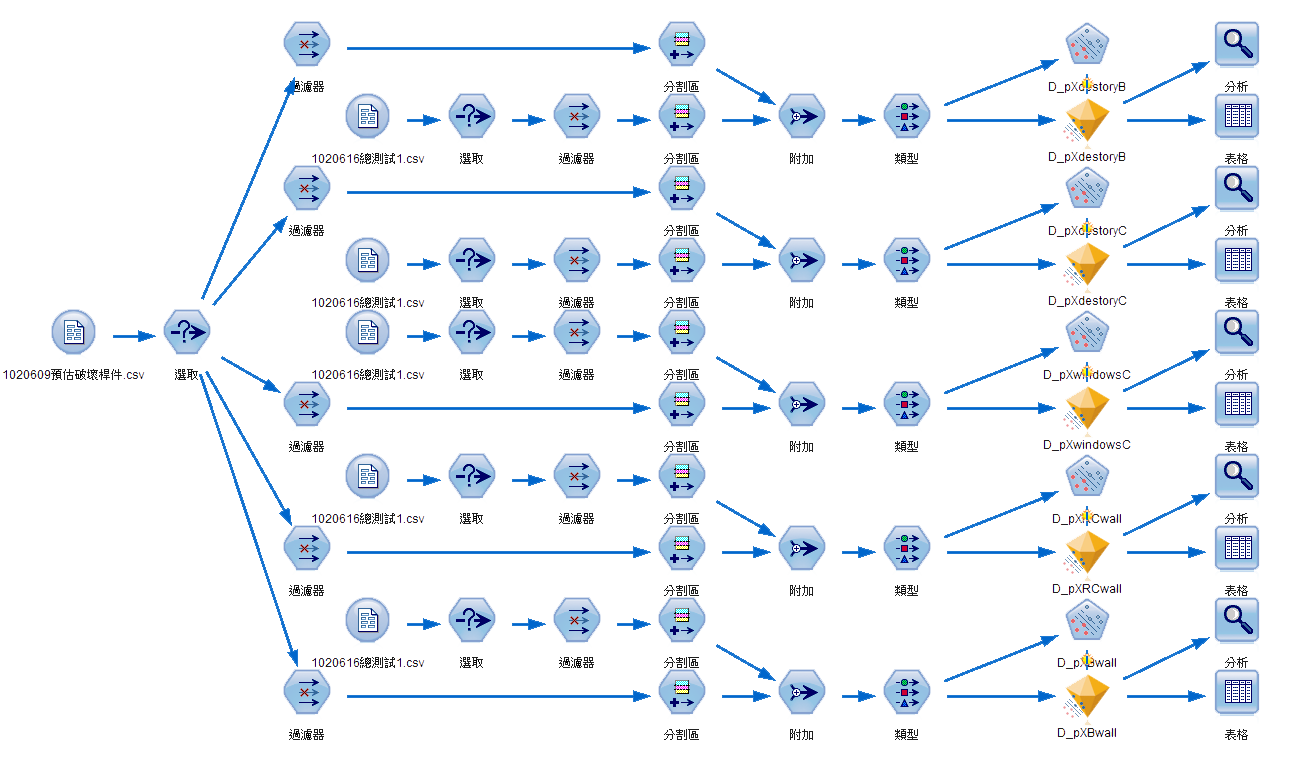
\includegraphics[width=1.0\textwidth]{figures/crack-flow.png}
    \caption{構件破壞模型探勘流程} 
    \label{fig:crack-flow}
  \end{center}
\end{figure}


\setlength{\tabcolsep}{2em}
{\renewcommand{\arraystretch}{1.5}
\begin{table}[hbtp]
  \begin{center}
    \caption{破壞構件關係模型結果}
    \label{tab:comp_result}
    \begin{tabular}{l c c}
    	\hline
    	破壞元件 & 資料集 & 正確率 \\
    	\hline
    	\multirow{2}{*}{X 正向樑破壞} & 訓練集 & 76.97\% \\
    	\cline{2-3} & 測試集 & 82.14\% \\
    	\hline
    	\multirow{2}{*}{X 正向柱破壞} & 訓練集 & 86.52\% \\
    	\cline{2-3} & 測試集 & 86.90\% \\
    	\hline
    	\multirow{2}{*}{X 正向窗台柱破壞} & 訓練集 & 79.21\% \\
    	\cline{2-3} & 測試集 & 77.38\% \\
    	\hline
    	\multirow{2}{*}{X 正向~RC~牆破壞} & 訓練集 & 99.32\% \\
    	\cline{2-3} & 測試集 & 98.25\% \\
    	\hline
    	\multirow{2}{*}{X 正向磚牆破壞} & 訓練集 & 80.34\% \\
    	\cline{2-3} & 測試集 & 80.95\% \\
    	\hline
    \end{tabular}
  \end{center}
\end{table}
}


根據表~\ref{tab:comp_result}~所示,可以發現五種構件的破壞關係模型的表現均不錯,正確率都有超過~75\%~,甚至~80\%~,其中~RC~牆的部分正確率特別高,其原因是校舍中有~RC~牆的校舍比例偏低,因此關係模型在訓練時會找到校舍是否有~RC~牆和是否有~RC~牆破壞的高度關聯性,因此沒有~RC~牆的校舍都很容易就判斷為沒有~RC~牆破壞,實際上在~297~棟校舍當中,只有~39~棟校舍有~RC~牆,如果只看這~39~棟校舍,則正確率有~89.7\%,且沒有~RC~牆的校舍當中,只有一棟校舍判斷錯誤。

%本探勘模型使用支援向量機並分別針對耐震詳細評估資料表之性能點狀態下最嚴重破壞樓層之主要破壞桿件及其破壞模式進行預測,其各項之預測正確率如下: \\ \indent
%X~正向樑破壞 97.06\% \\ \indent
%X~正向柱破壞 100\% \\ \indent
%X~正向窗台柱破壞 94.12\% \\ \indent
%X~正向 RC 牆破壞 100\% \\ \indent
%X~正向磚牆破壞 82.6\% \\ \indent


%beam, 139
%  train  5/262
%  test   1/34

%column, 227
%  train  36/262
%  test   0/34

%window, 228
%  train  2/262
%  test   2/34

%rc wall, 13
%  train  5/262
%  test   0/34

%brick wall, 175
%  train  48/262
%  test   5/34

% 最後並根據每棟校舍於性能點狀態下,各項破壞構件其破壞模式進 行正確率之計算,根據耐震詳細評估資料表內有五項破壞構件之欄位,因此本分析假設該校舍於每項破壞構件之欄位如預測正確,則加正確率百分之二十,共五項欄位,如各項接預測正確,則該校舍針對其性能點狀態下最嚴重破壞樓層之主要破壞桿件及其破壞模式之預測正確率為百分之百。其 34 棟總體校舍針對 5 種破壞構件及其破壞模式之平均預測正確率為 95.3\%。本預測目標其欄位屬性為類別型態,因此無法以其他評估指標進行比較,一般評估指標只能用來評估數值型資料。34 棟校舍於破壞構件及其破壞模式之預測資料與結果如,X 正向樑破壞於表 5.6 中欄位名稱為 D\_pXdestoryB,X 正向柱破壞於表 5.6 中欄位名稱為~D\_pXdestoryC,X 正向窗台柱破壞於表 5.6 中欄位名稱為 D\_pXwindowsC,X 正向 RC 牆破壞於表 5.6 中欄位名稱為 D\_pXRCwall,X 正向磚牆破壞於表 5.6 中欄位名稱為 D\_pXBwall,其餘之欄位說明如表 5.5。

	\renewcommand\thetable{\arabic{chapter}-\arabic{table}}
%\renewcommand\thefigure{\arabic{chapter}-\arabic{figure}}
\chapter{校舍資訊與補強經費之關係模型}
\label{cha:cob} 

校舍建築物的補強經費對於全國校舍的補強工作來說是非常重要的一個數值,和校舍的耐震能力並列,因其直接表示了主管機關要讓該棟校舍符合耐震安全規範所需要的成本,教育部為了提升全國高中職及中小學校舍耐震能力,歷年來已經訂定及執行了「加速國中小老舊校舍及相關設備補強整建計畫」及「加速高中職及國中小老舊校舍及相關設備補強整建計畫」。教育部將計畫委託國震中心執行,國震中心與教育部研擬商討後,再訂出執行計畫交由各縣市政府辦理。計劃的訂定需要資料的輔助,計劃的執行也需要定期的計劃報告以掌握計劃的執行進度與效力。全國校舍總數,經目前耐震資料庫中校舍普查作業已記錄之校舍數量統計共有~24930~棟,如果考慮尚未執行校舍普查作業之校舍,其實際校舍總數將更多。面對如此大量之校舍,進行總體或縣市為單位之經費估算,需耗費大量時間與人力進行估算與統計。且依照目前「高中職及國中小校舍結構耐震能力詳細評估作業規範」\cite{ncree2013moe}~規定,主管機關須等到詳細評估之承攬廠商提送期末報告書,才能得知該校舍較精確之可能補強費用。由此可知,校舍補強經費的取得也是一個非常耗時且困難的流程,要提早在校舍進入詳細評估前就推估出校舍的補強經費,以往只能透過較為簡單的經驗公式推估,

目前主管機關在提撥補強校舍的耐震能力計畫的經費時,是每個年度依據需求估算,編列該年度的固定經費,根據教育部公布九十九年九月十六日修正之國中小校舍「補強工程」之經費支用範圍及參考單價計價方式,「補強工程」費用,包含了「直接補強工程費」、「合理之間接修復費」、「工程管理費」、「補強設計及監造費」等費用支出。依公告之估價方式將校舍分為「已完成補強設計」與「尚未完成補強設計」,歸類為「已完成補強設計」之校舍,其補強工程經費依補強設計審查通過或補強設計報告之金額,教育部原則將據 以如數核定補助經費。但其補強工程單價超出~$4000~\text{元}/m^2$~者,則應經補強設計期末審查或特別審查通過並附審查意見表,始能獲教育部如數核定補助經費;否則將依單價~$4000~\text{元}/m^2$~核定補助經費。歸類為「尚未完成補強設計」之校舍(凡未附補強設計審查意見表、未附補強設計報告重點摘要部分、或佐證資料不齊全者,皆屬尚未完成補強設計):其「補強工程」之參考單價計價方式依其總樓地板面積所屬級距範圍之不同,分別計算如表~\ref{tab:cost_result_table}\cite{ncree2010moe}~所示,其中「計價面積」係由「實際面積」以無條件進位為~2~的倍數之方式轉換而成;因此計價面積為~2~的倍數且為整數。例如:實際面積~$601~m^2$~,應轉換為計價面積~$602~m^2$。

\setlength{\tabcolsep}{1em}
{\renewcommand{\arraystretch}{1.5}
\begin{table}[hbtp]
  \begin{center}
    \caption{補強工程參考單價之計價方式}
    \label{tab:cost_result_table}
    \begin{tabular}{l l}
      \hline
      建築物樓地板總面積 & 補強工程費用計算方式 \\
      \hline
      不足~$600~m^2$ & $\text{實際面積} \times 4000 \text{元}/m^2$ \\
      $600~m^2$~以上,不足~$3600~m^2$ & $\text{計價面積} \times (-0.5 \times \text{計價面積} + 4300) \text{元}/m^2$ \\
      $3600~m^2$~以上 & $\text{實際面積} \times 2500 \text{元}/m^2$ \\
      \hline
      \end{tabular}
  \end{center}
\end{table}
}

此一補強工程參考計價方式的主要依據是校舍的樓地板面積,但是實際影響補強經費的因素應該不只是校舍的樓地板面積,建築物的牆柱設計、施工品質、建造年代、不足的耐震能力等,對於補強的方式應該都有很大的影響,也間接的影響到補強經費,因此用此計價方式所得到的補強費用預估值是可靠度相對不足的數字,而此一預算編列的方式,是每年編列固定額度的預算,編列的年度預算難以在事後追加,使用可靠度不足的數字作為參考,會讓編列的預算與實際需求失準,而且每年固定的預算已經會讓每個年度能夠補強的校舍數量有所限制,對於不知何時會再發生的地震威脅,絕對是希望能夠儘快將最危險的校舍找出並做出對應處置,因此校舍耐震能力補強的經費編列和分配的影響就非常大,不過實際上在編列預算時,大部分校舍可能都還沒進行詳細評估、也還沒有建議的補強方案,因此只能透過參考資料和初步評估的資料來估算,如果可以在編列預算時,就能推估每間校舍的耐震能力、補強可能需要的經費,那麼主管機關在編列和分配預算的時候就可以非常有效率的來編列,因此本研究還試著找出校舍的基礎設計參數與其補強經費間的關係模型,透過這個模型,應該可以從校舍的初步評估資料得到一個可靠度較高的補強經費推估值。


\section{資料前處理}

本分析其構想為建立校舍評估階段初期之已調查資料以及評估階段後期結果間之關係模型。校舍耐震之補強工程經費須等到工程完成且承攬廠商提送竣工報告才能得知最後實際施工所花經費,因研究目標為達成前期預測之目的,所以需挑選補強施工以前之補強階段資料。校舍耐震評估與補強之流程如圖~\ref{fig:FLOW}~,可知進行補強施工之前尚須進行校舍普查、初步評估、詳細評估與補強設計,經了解各階段評估作業之內容與用途,校舍普查執行之人員為各大專院校之土木系學生 協助執行,且其所記錄之資料也較其他各階段為少,補強設計為補強施工之上一階段,根據「高中職及國中小校舍結構耐震能力補強設計作業 規範」規定,補強設計成果報告書中須編製工程預算書,因此即可於補強設計階段得知該補強工程之所需經費。為達研究之預測目的,本研究將採用初步評估與詳細評估(不含耐震補強方案)結果做為本探勘模型之選擇資料,並以典型校舍、鋼筋混凝土建築、單邊走廊且廊外無柱、無地下室、補強工程經費介於~100~至~1000~萬之間、初步評估與詳細評估均顯示為已送出之資料做為此模型資料選擇之條件篩選。

本模型採用初步評估與詳細評估(不含耐震補強方案)資料表中之資料做為本探勘模型之選擇資料,並以典型校舍、鋼筋混凝土建築、單邊走廊且廊外無柱、無地下室、補強工程經費介於~100~至~1000~萬之間、初步評估與詳細評估均顯示為已送出之校舍資料做為此模型資料選擇之條件篩選。模型經資料選擇與前處理之後建立資料集,下一步即是進行模型屬性之選擇,建立屬性集,本模型挑選之屬性集如下:

\begin{multicols}{2}
\begin{itemize}
\item 一樓樓地面積
\item 柱等效強度
\item 軟弱層顯著性
\item 裂縫鏽蝕滲水等程度
\item 短柱嚴重性
\item 調整因子
\item 二樓樓地板面積深
\item 二樓樓地板面積長
\item 樓層數
\item 二樓以上樓地板面積
\item 一樓教室柱根數
\item 一樓走廊外柱斷面積和
\item 非結構牆
\item X正向樑破壞
\item X正向柱破壞
\item X正向窗台柱破壞
\item X正向磚牆破壞
\item X正向性能點之屋頂最大位移
\item X正向性能點之等效基本週期
\item X正向性能點之基底剪力
\item 校舍耐震容量需求比
\item[]
\end{itemize}
\end{multicols}

以下為本預測模型屬性集內之屬性介紹與選擇說明:

\begin{description}
  \item[一樓樓地面積]
  依據教育部現行之補強工程計價公式如表~\ref{tab:cost_result_table}~,其經驗公式以樓地板面積為主要參數,而其可靠度雖然較差,但仍然是主管機關一個重要的參考數值,本分析所建立之模型為補強工程經費與校舍設計參數間的關係,而校舍之樓地板面積也是一個非常重要的設計參數,可以代表校舍結構之規模,校舍的載重,也隱含了校舍如果需要補強時,其工程規模大小之資訊在其中,因此本分析將此屬性拿來作為建立此關係模型之輸入屬性。
  \item[柱等效強度]
  柱之等效強度~$T_{AC}$~其計算公式為:

  \begin{equation}T_{AC} = (4+1.8NF)ClaAc+(2.4+1.08NF)CorAc+2.6InsAc\end{equation} 

  其中~$NF$~為樓層數,~$ClaAc$~為一樓教室柱總斷面積,~$CorAc$~為一樓走廊外柱總斷面積,~$InsAc$~為一樓隔間柱總斷面積,其公式為根據三種類結構柱之單位斷面積極限剪力牆度計算公式~\cite{su2008master}~之加總,本分析將此屬性加入探勘模型之最初原因為該公式內有教室柱、走廊外柱與隔間柱於一樓的總斷面積,而此一數值和,並且因補強施工其所補強之面積愈大其所花錢就愈多。本分析經建立多組模型與各種屬性集之測試均發現該屬性對模型之預測結果有一定影響。
  \item[軟弱層顯著性]
  \cite{ncree03049}~若結構物之一樓因為使用性等考量,而使得二樓以上~RC~牆或磚牆於一樓中斷,致使一樓之極限層剪力強度與勁度降低,將造成地震力作用時變形集中,以致於韌性用盡,建築物就發生軟弱層破壞。故本表格依據牆體中斷的程度折減其對應之耐震能力,若~2/3~以上牆體中斷,則耐震能力折減為~0.8~倍;若~1/3~至~2/3~之牆體中斷,則耐震能力折減為~0.9~倍;若~1/3~以下之牆體中斷,則不折減其耐震能力。依此敘述得知軟弱層顯著性會影響結構物之耐震能力,結構物之耐震能力愈低,極可能所需補強之工程花費就愈高,因此本分析將此屬性納入本屬性集。
  \item[裂縫鏽蝕滲水等程度]
  \cite{ncree03049}~此為初步評估之調整因子之一,建物若有裂縫鏽蝕滲水等情形會影響耐震能力,耐震能力愈差就有可能提升所需花費之工程經費,且此一資訊是最能夠帶表現社現況之資料,因此本分析將之納為輸入屬性。
  \item[短柱嚴重性]
  \cite{ncree03049}~此為初步評估之調整因子之一,而可知短柱現象為影響校舍耐震能力原因之一,因此將之納入輸入屬性。
  \item[調整因子]
  \cite{ncree03049}~典型校舍初步評估表之六項調整因子調查項目,其功能為對初步評估耐震能力產生增減,包括:平面及立面對稱性、軟弱層顯著性、裂縫鏽蝕滲水等程度、變形程度、平面耐震性以及短柱嚴重性,定義~$q_1$~至~$q_6$~分別代表六項調整因子,其中軟弱層顯著性、裂縫鏽蝕滲水等程度和短柱嚴重性三項調整因子因對耐震能力之影響較為直接,所以也分別被納本分析之輸入屬性,而除此六項調整因子外,還有定義一整體調整因子~$Q$~為上述六項調整因子之乘積,整體調整因子代表所有調整因子對於耐震能力的折減或增加的幅度,其物理意義為校舍的現況對於校舍耐震能力影響的程度,對於校舍耐震能力來說也是很重要的一個參數,且經測試後證實該屬性對預測之正確性有提升,因此本分析也將其納入輸入屬性。
  \item[二樓樓地板面積深、深]
  依據教育部現行之補強工程計價公式如表~\ref{tab:cost_result_table}~,其公式以樓地板面積為主要參數,又面積之算法為長乘以寬(深),因此亦可將它視為影響校舍補強工程經費的因素之一。本分析所預測之目標為實際施工之工程總經費,與計價公式所估經費有直接關聯性,因此本分析將此二屬性拿來作為本預測模型之輸入屬性。
  \item[樓層數]
  樓層數愈高其總樓地板面積愈多,其總樓地板面積愈多,依補強工程計價公式如表~\ref{tab:cost_result_table}~。其工程經費預算就可能愈多,因此樓層數亦可視為影響工程經費之影響原因之一。
  \item[二樓以上樓地板面積]
  依據教育部現行之補強工程計價公式如表~\ref{tab:cost_result_table}~,其公式以樓地板面積為主要參數,本分析所預測之目標為實際施工之工程總經費,補強工程計價公式為經費預算之計算方式,估算出來之經費預算往往與實際施工所花經費不太一樣,預算可能高於實際施工也可能低於實際施工,但因為目標都是估算工程經費,因此本分析將此屬性拿來作為本預測模型之輸入屬性。
  \item[一樓教室柱根數]
  由校舍教室柱之數量可以間接得知校舍樓地板面積之大小或規模,且柱子的數量可以間接代表校舍乘載能力的大小,因此本分析將之視為影響工程經費之因素之一,經將此屬性納入探勘模型中測試後,也確實發現此屬性對預測之正確率有一定之提升。
  \item[一樓走廊外柱斷面積和]
  走廊外柱總斷面積愈大其意義可能有二:其一,斷面積愈大可能代表樓地板面積愈大,而根據補強經費估算的經驗公式,樓地板面積愈大其施工所需經費即可能愈高。其二,如果校舍樓地板面積大小一樣,但其廊外柱斷面積和比較大,代表其走廊外柱可能斷面積比較大,如果要進行擴柱補強工法,其工程所花經費就會比較高。綜合以上原因,本分析即嘗試將此屬性納入探勘模型中,並且經測試後效果不錯因此保留此屬性。
  \item[非結構牆]
  此屬性為記錄該校舍,有無非結構牆,並於分析時所建立模型是否有將該非結構牆模擬成其他等值桿件進入結構模型內。因有無非結構牆可能會影響校舍之耐震能力,而本分析之探勘目標包括了磚牆和~RC~牆是否破壞,,因此將之加入輸入變數。
  \item[X~正向樑破壞、X~正向柱破壞、X~正向窗台柱破壞、X~正向磚牆破壞]
  此四屬性為詳細評估資料表中之記錄欄位,記錄詳評後校舍可能優先破壞的構件以及其破壞的形式,此分析中根據實際詳細評估資料中的破壞趨勢選擇了包括~X~正向樑、~X~正向柱破壞、~X~正向窗台柱以及~X~正向磚牆四種構件的破壞模式,區分為無破壞、剪力破壞、撓剪破壞、撓曲破壞四種破壞形式,不同之破壞形式其需補強的方式會有所不統,其所需經費也不一樣,因此本分析將之列為本模型之輸入屬性。
  \item[X~正向性能點之屋頂最大位移]
  \cite{ncree08035}進行詳細評估時,若採用推垮分析,則該欄位則須依~X~及~Y~方向分別輸入屋頂最大位移值。本分析僅挑選採用推垮分析之校舍進行建模,因屋頂之最大位移為影響校舍耐震能力的因素之一,因此也將該屬性列入。
  \item[X~正向性能點之等效基本週期]
  \cite{ncree09015}基本週期為結構物等效單自由度系統的動力參數(性能目標地表加速度),此單自由度系統在性能目標地表加速度的設計地震作用下,其動力反應將是已設定的性能需求,因此基本週期亦是影響耐震能力評估結果的因素之一。
  \item[X~正向性能點之基底剪力]
  基底剪力為側推分析中計算容量曲線之重要參數之一,校舍之耐震能力可能影響補強之工程經費,因此本分析嘗試將此屬性放入本模型中進行測試,其結果對模型預測之正確率有提升,因此將它保留至屬性集之中。
  \item[校舍耐震容量需求比]
  \cite{ncree09026}校舍建築物進行耐震初步評估後,得到一耐震指標分數~$Is$~,此耐震指標可作為是否需進入下一階段評估工作的參數,同樣地,經由專業人員完成詳細評估後,得到建築物長短向最大可抵抗之地表加速度,除以該校舍~475~年迴歸週期設計地表加速度,稱之耐震容量需求比(Capacity Demand Ratio,CDR),此數值若小於~1~時,則判定該棟建築須進行補強;反之,該棟建築耐震能力暫無疑慮,但仍須定期檢視。根據上述得知~$CDR$~可視為該校舍之耐震能力與正常安全值之距離,如果數值小於~1~且離~1~愈遠,代表需替該校舍提升的耐震能力愈多,所需花的經費就愈多,因此亦可視為影響補強工經費之因子。
\end{description}

至於探勘的目標,補強經費還可以細分為直接費用和間接費用,間接費用包括向專案管理成本之類的費用,直接費用則是和補強工程直接相關的費用,又可以分為結構補強費用和非結構補強費用,其中,和結構相關,最能夠直接反應校舍結構的耐震能力的經費數值是結構補強費用,不過考量到模型的實用性,加上資料庫內之資料也包含校舍現況等資訊,而一般的專案管理費用也是照總工程款的固定比例,應該有足夠的資訊能夠探勘出總補強經費與校舍參數間之關係模型,因此本研究所挑選的探勘目標便是總補強經費。

\section{資料探勘}

本分析採用類神經網路與~CHAID~決策樹進行資料探勘之建模,選擇此二種探勘方法,主因為本分析之預測目標,總工程經費為連續數值,最適合使用的探勘演算法為迴歸演算法,因此挑選其中應用範圍最廣的類神經網路做為基準,另外屬於決策樹方法分支之~CHAID~決策樹經初步測試應用於本分析之預測目標,其表現不錯,因此本分析以此二種探勘方法,使用前處理完之~235~筆資料,將整體資料採亂數選取方式分為~85\%~為訓練區與~15\%~為測試區,類神經網路之設定為使用~Multilayer Perceptron(MLP)之網路形式,並讓~SPSS Modeler~自動計算隱藏層數量及各層節點數,訓練~15~分鐘,然後挑出表現最佳的一組神經網路。CHAID~決策樹之模型設定為:最大決策樹深度為五層,停止條件為決策節點之資料筆數為總數之~1\%,SPSS Modeler~之節點架構如圖~\ref{fig:cob-flow}~所示,模型之訓練結果如表~\ref{tab:cost_result}。

\begin{figure}[hbtp]
  \begin{center}
    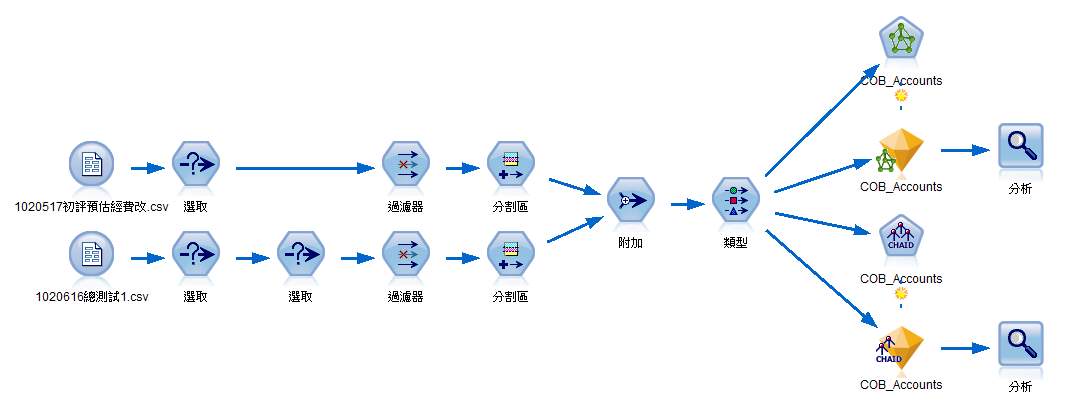
\includegraphics[width=1.0\textwidth]{figures/cob-flow.png}
    \caption{補強經費模型探勘流程} 
    \label{fig:cob-flow}
  \end{center}
\end{figure}

%先行根據既有知識挑選資料集內之欄位並配合使用試誤法直到找出最佳做為探勘模型之屬性集,做為模型訓練方法。

%最後再挑一組結果較好之模型與屬性集保留。本模型之訓練結果如表~\ref{tab:cost_result},因本模型之整體資料較少,其結果之線性相關程度目前呈現比較低。

{\renewcommand{\arraystretch}{1.5}
\begin{table}[hbtp]
  \begin{center}
    \caption{補強經費關係模型結果}
    \label{tab:cost_result}
    \large
    \begin{tabular}{l c c c c}
      \hline
       & \multicolumn{2}{c}{ANNs} & \multicolumn{2}{c}{CHAID} \\
       & Training & Testing & Training & Testing \\
      \hline
%    $R$ & 0.812 & 0.949 & 0.718 & 0.874 \\
      $R^2$ & 0.659 & 0.900 & 0.516 & 0.764 \\
      MAPE & 25.01\% &34.83\% & 27.09\% & 39.73\% \\
      \hline
      \end{tabular}
  \end{center}
\end{table}
}

\section{結果}

本資料探勘分析結果得到兩個可以從校舍基本設計資料得到其補強所需經費之關係模型,分別為使用類神經網路及 CHAID 決策樹所探勘得到,表~\ref{tab:cost_result_2}~為此兩二模型不分測試訓練集之~$R^2$~與~MAPE~,其中,第三欄之~NCREE~指使用國震中心參考計價方式所得到的補強經費。CHAID~模型之推估值與實際值之比較如圖~\ref{fig:cob-chaid-vs}~所示,而類神經網路模型之推估值與實際值之比較如圖~\ref{fig:cob-ann-vs}~所示。兩者比較可以發現~CHAID~因為其知識形式為決策樹之特性,所得到的推估值只有數種可能性,造成其~MAPE~較高,但是其在圖~\ref{fig:cob-chaid-vs}~上所呈現之線性關係,表示此模型仍保有正確之關係於模型之中,而根據圖~\ref{fig:cob-chaid-vs}~可以發現其誤差方向之分佈尚且平均,計算~235~棟校舍之平均誤差量僅為~11066~元,類神經網路模型之平均誤差量則為~33512~元,顯示此一模型尚可以用在大量校舍之整體補強預算評估上,然而如果要推估單棟校舍之補強經費,則建議使用類神經網路探勘所得到之模型,根據圖~\ref{fig:cob-ann-vs}~可以發現其數據較為集中,只是其趨勢與~$y = \hat{y}$~之目標趨勢方向稍有不同,表示此模型有確實的呈現校舍設計參數與其補強費用間的關係趨勢,然而仍然有些影響補強經費的因素尚未被找出。最後如果將此模型與表~\ref{tab:cost_result_table}~之公式做比較,也可以發現其表現優異許多,使用公式計算所得到的補強預算推估值與實際數字比較之~$R^2$~為~0.54,而類神經網路所建立之關係模型的~$R^2$~為~0.69~,準確度確實較計價公式要高,與~Jafarzadeh\cite{jafarzadeh2013predicting}\cite{jafarzadeh2013application}~之研究結果相比,補強經費關係模型之~$R^2$~表現相同,然而本研究測試集之表現較好,穩定度較高。

{\renewcommand{\arraystretch}{1.5}
\begin{table}[hbtp]
  \begin{center}
    \caption{補強經費關係模型結果(不分測試集)}
    \label{tab:cost_result_2}
    \large
    \begin{tabular}{l c c c}
      \hline
       & ANNs & CHAID & NCREE \\
      \hline
     $R^2$ & 0.69 & 0.55 & 0.54 \\
     MAPE & 26.43\% & 28.91\% & 32.95\% \\
      \hline
      \end{tabular}
  \end{center}
\end{table}
}

\begin{figure}[hbtp]
  \begin{center}
    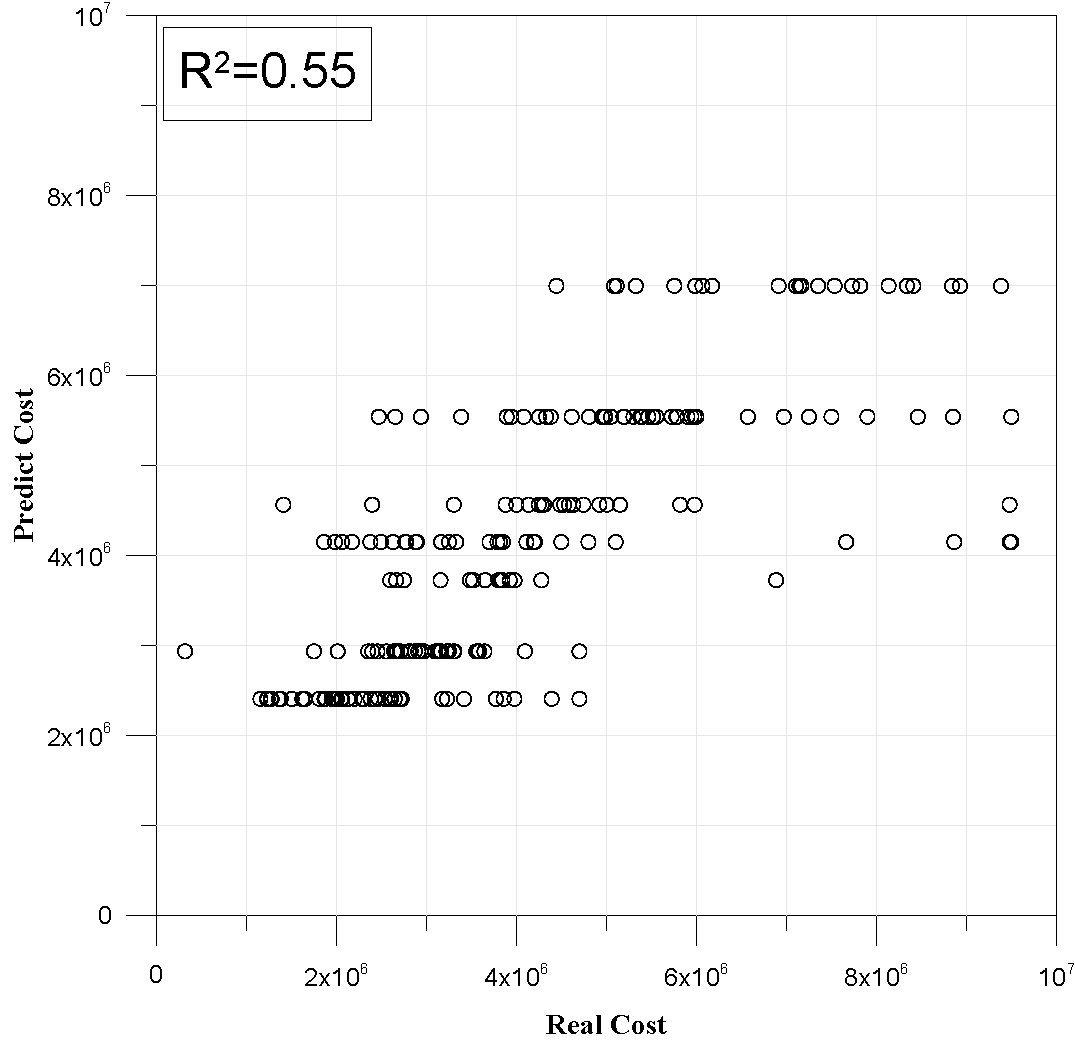
\includegraphics[width=0.7\textwidth]{figures/cob-chaid.pdf}
    \caption{補強經費實際值 vs CHAID 模型預估值} 
    \label{fig:cob-chaid-vs}
  \end{center}
\end{figure}


\begin{figure}[hbtp]
  \begin{center}
    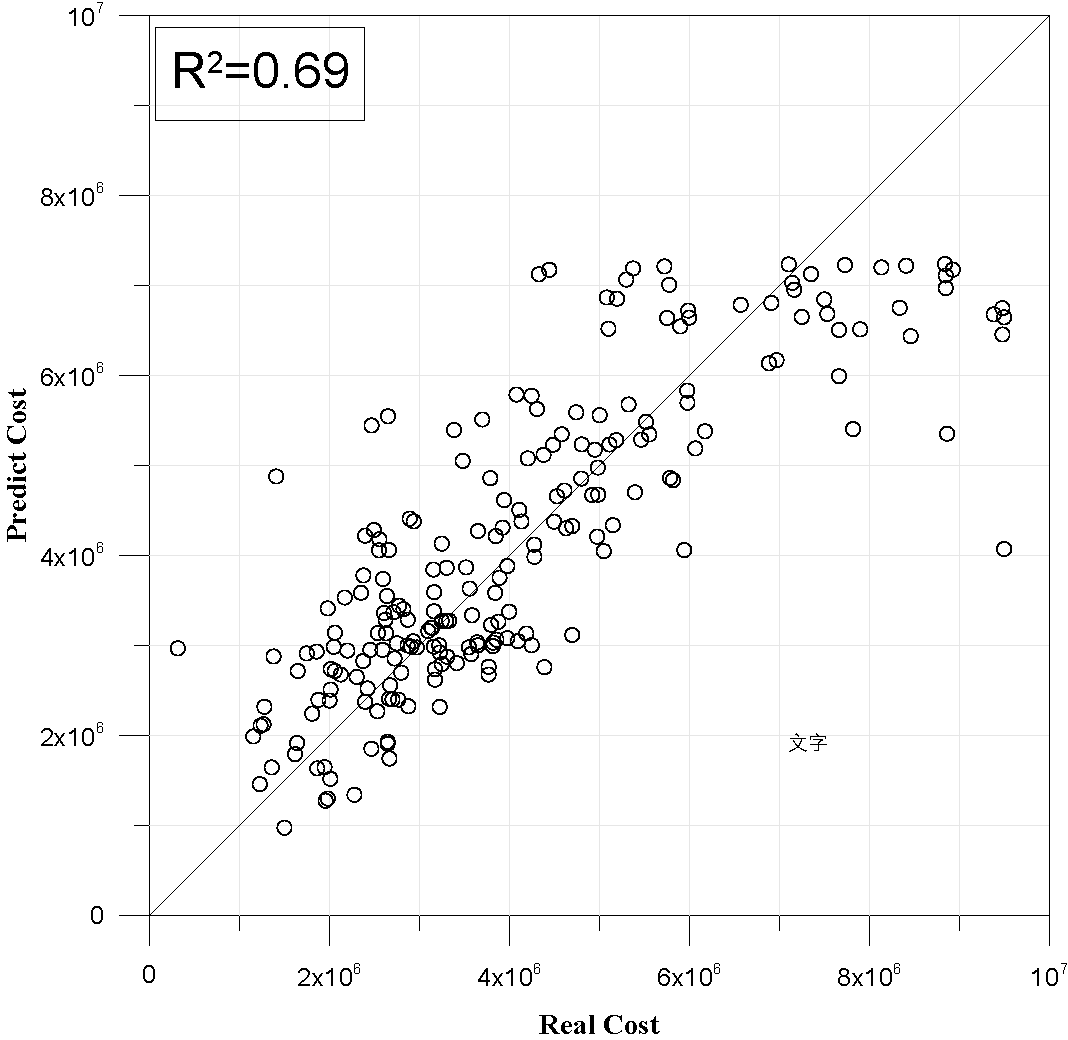
\includegraphics[width=0.7\textwidth]{figures/cob-ann.pdf}
    \caption{補強經費實際值 vs ANN 模型預估值} 
    \label{fig:cob-ann-vs}
  \end{center}
\end{figure}


%雖然相較於~CHAID~決策樹,類神經網路的表現較差,

%本分析用來判斷模型優劣的指標為~$R^2$~和~MAPE~,~MAPE~用來表示模型預測值的平均誤差,為一百分比索引值,數值越小表示模型品質越好,使用此一指標的主因在於可以用來評估此迴歸模型所估算之補強經費,其誤差可能造成之經費差距有多少,對於主管機關來說也是一個非常重要的參考依據,根據表~\ref{tab:cost_result}~,類神經網路和~CHAID~決策樹的表現均很接近,且其測試集的表現顯示此二模型均有其可靠性,最後選擇使用類神經網路作為最後挑選的模型,不分訓練測試集重新訓練建立關係模型,結果其~MAPE~為~31.8\%~,~$R^2$(相關係數)為~0.9004~,可以發現~$R^2$~的表現很好,表示此模型有確實的呈現校舍設計參數與其補強費用間的關係趨勢,然而~MAPE~表現較差,顯示仍然有些影響補強經費的因素尚未被找出。







	\input{sections/conclusion.tex}

	%----------------------------------------------------------------------------------------------------------------------------------------------------------
	% back pages 後頁
	% 包括參考文獻、附錄、自傳
	% 實際內容由
	%    my_bib.bib, my_appendix.tex, my_vita.tex
	% 決定
	% ntust_backpages.tex 此檔只提供整體架構的定義,不需更動
	% 在撰寫各章草稿時,可以把此部份「關掉」,以節省無謂的編譯時間。
	%\bibliographystyle{unsrt} 
	%
% this file is encoded in utf-8
% v1.7

%%% 參考文獻
\newpage
%\bibliographystyle{unsrt}
\cleardoublepage
\phantomsection
\addcontentsline{toc}{chapter}{\nameRef}
\renewcommand{\bibname}{\protect\makebox[5cm][s]{\nameRef}}
%  \makebox{} is fragile; need protect
%\bibliographystyle{unsrt} 
\bibliographystyle{ieeetr}  % 使用 IEEE Trans 期刊格式
%\bibliographystyle{unsrt}
\bibliography{my_bib}  %reference 所需的bib檔
%\bibliographystyle{unsrt} 

%%% 附錄
%
% this file is encoded in utf-8
% v1.7
%%% 每一個附錄 (附錄一、附錄二、...) 都要複製此段附錄編排碼做為起頭
%%% 附錄編排碼 begin >>>

\includepdfset{pages=-,pagecommand=\thispagestyle{AppendixPage}}

\newpage
\chapter*{附錄一:典型校舍初步評估表} % 修改附錄編號與你的附錄名
\label{appendix-pe}
\addcontentsline{toc}{chapter}{附錄一:典型校舍初步評估表} %建議此內容應與上行相同
\renewcommand{\thechapter}{一} % 如果是附錄二,則內容應為{二}

\setcounter{equation}{0} 
\setcounter{figure}{0} 
\setcounter{footnote}{0} 
\setcounter{section}{0} 
\setcounter{subsection}{0}
\setcounter{subsubsection}{0}
\setcounter{table}{0} 
%%% <<< 附錄編排碼 end

% 附錄內容開始
見下頁。

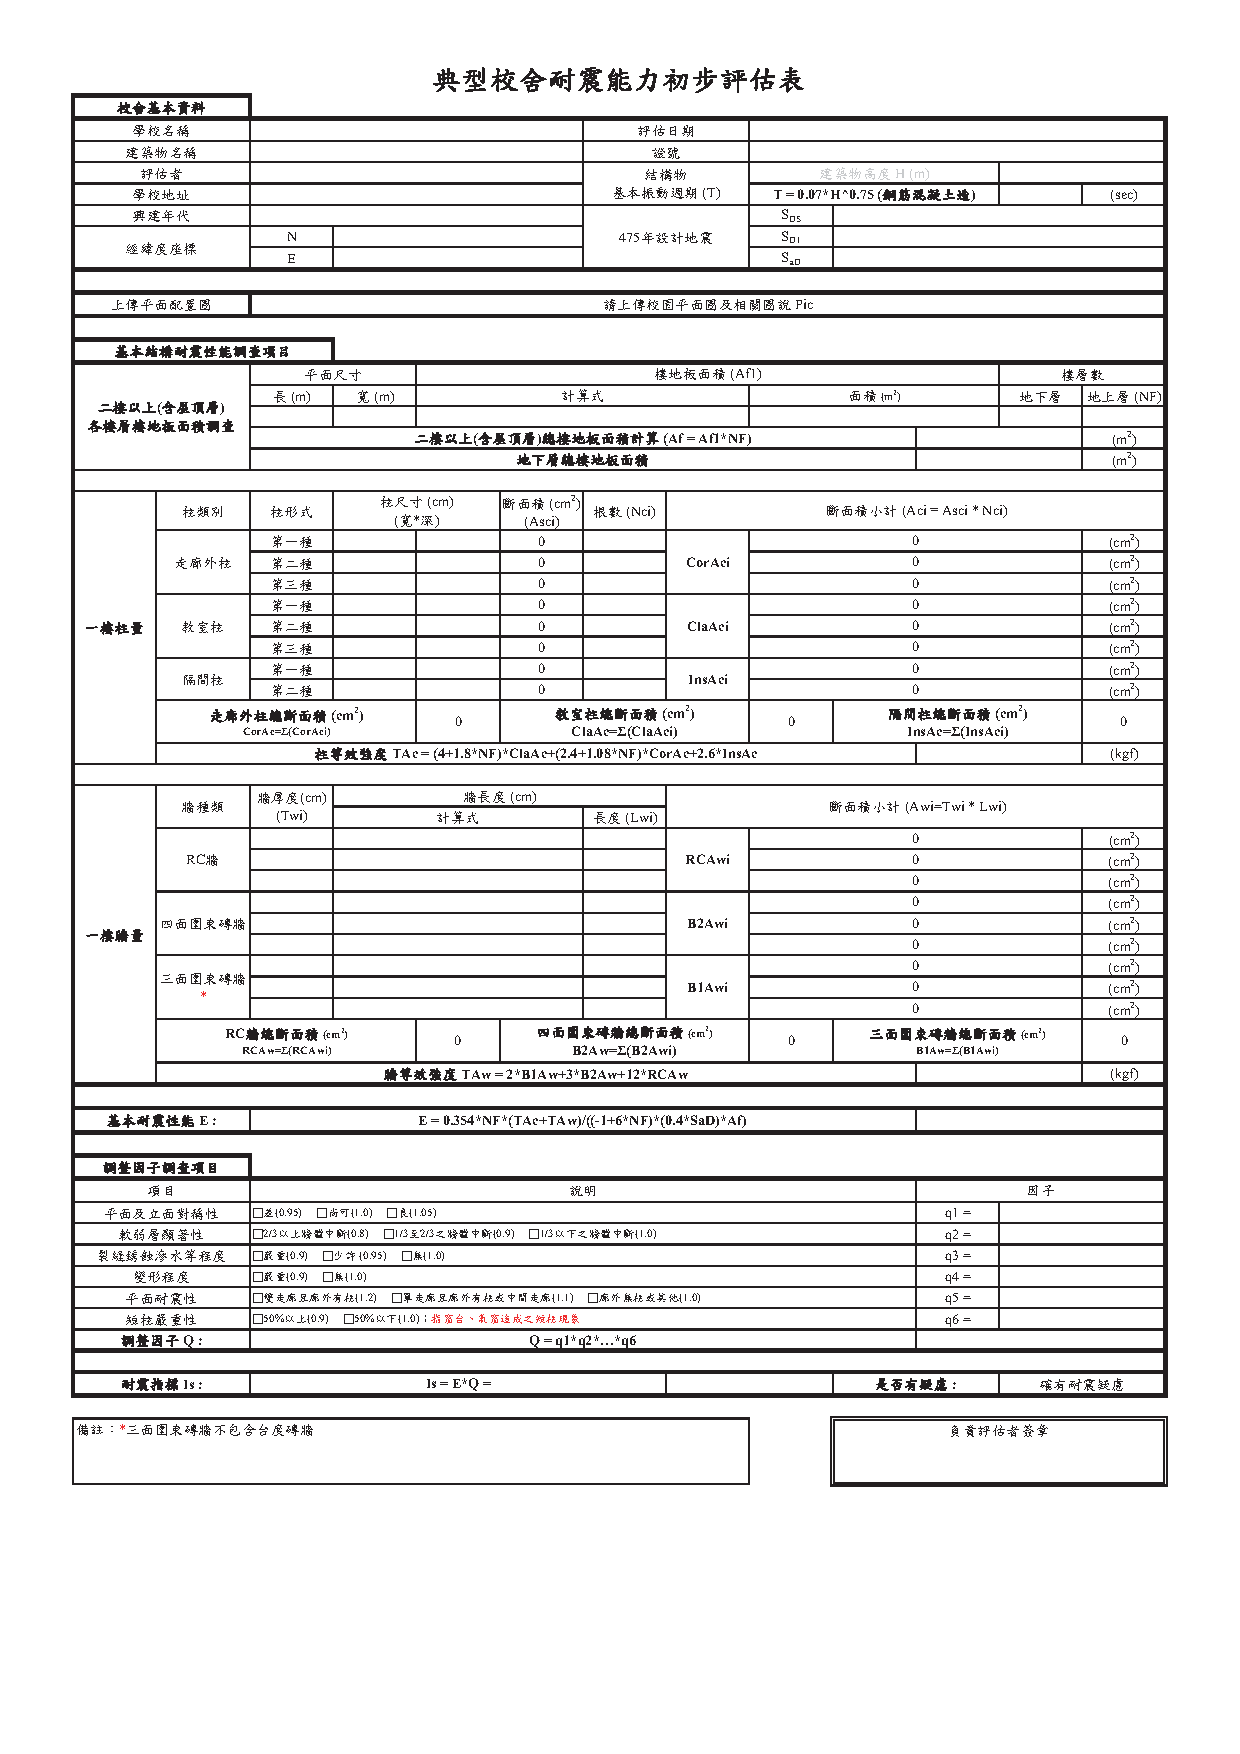
\includepdf[fitpaper=true,scale=0.95]{appendix/20120516-Preliminary-Typical.pdf}

%%% 如果有附錄二、三、...,則在此繼續加上「附錄編排」碼
% 每一個附錄會自動以新頁開始

\newpage
\chapter*{附錄二:典型校舍詳細評估表} % 修改附錄編號與你的附錄名
\label{appendix-de}
\addcontentsline{toc}{chapter}{附錄二:典型校舍詳細評估表} %建議此內容應與上行相同
\renewcommand{\thechapter}{二} % 如果是附錄二,則內容應為{二}

\setcounter{equation}{0} 
\setcounter{figure}{0} 
\setcounter{footnote}{0} 
\setcounter{section}{0} 
\setcounter{subsection}{0}
\setcounter{subsubsection}{0}
\setcounter{table}{0} 
%%% <<< 附錄編排碼 end

% 附錄內容開始
見下頁。


\includepdf[fitpaper=true,scale=0.95]{appendix/detailed-evaluation.pdf}


\newpage
\chapter*{附錄三:典型校舍補強設計表} % 修改附錄編號與你的附錄名
\label{appendix-re}
\addcontentsline{toc}{chapter}{附錄三:典型校舍補強設計表} %建議此內容應與上行相同
\renewcommand{\thechapter}{三} % 如果是附錄二,則內容應為{二}

\setcounter{equation}{0} 
\setcounter{figure}{0} 
\setcounter{footnote}{0} 
\setcounter{section}{0} 
\setcounter{subsection}{0}
\setcounter{subsubsection}{0}
\setcounter{table}{0} 
%%% <<< 附錄編排碼 end

% 附錄內容開始
見下頁。

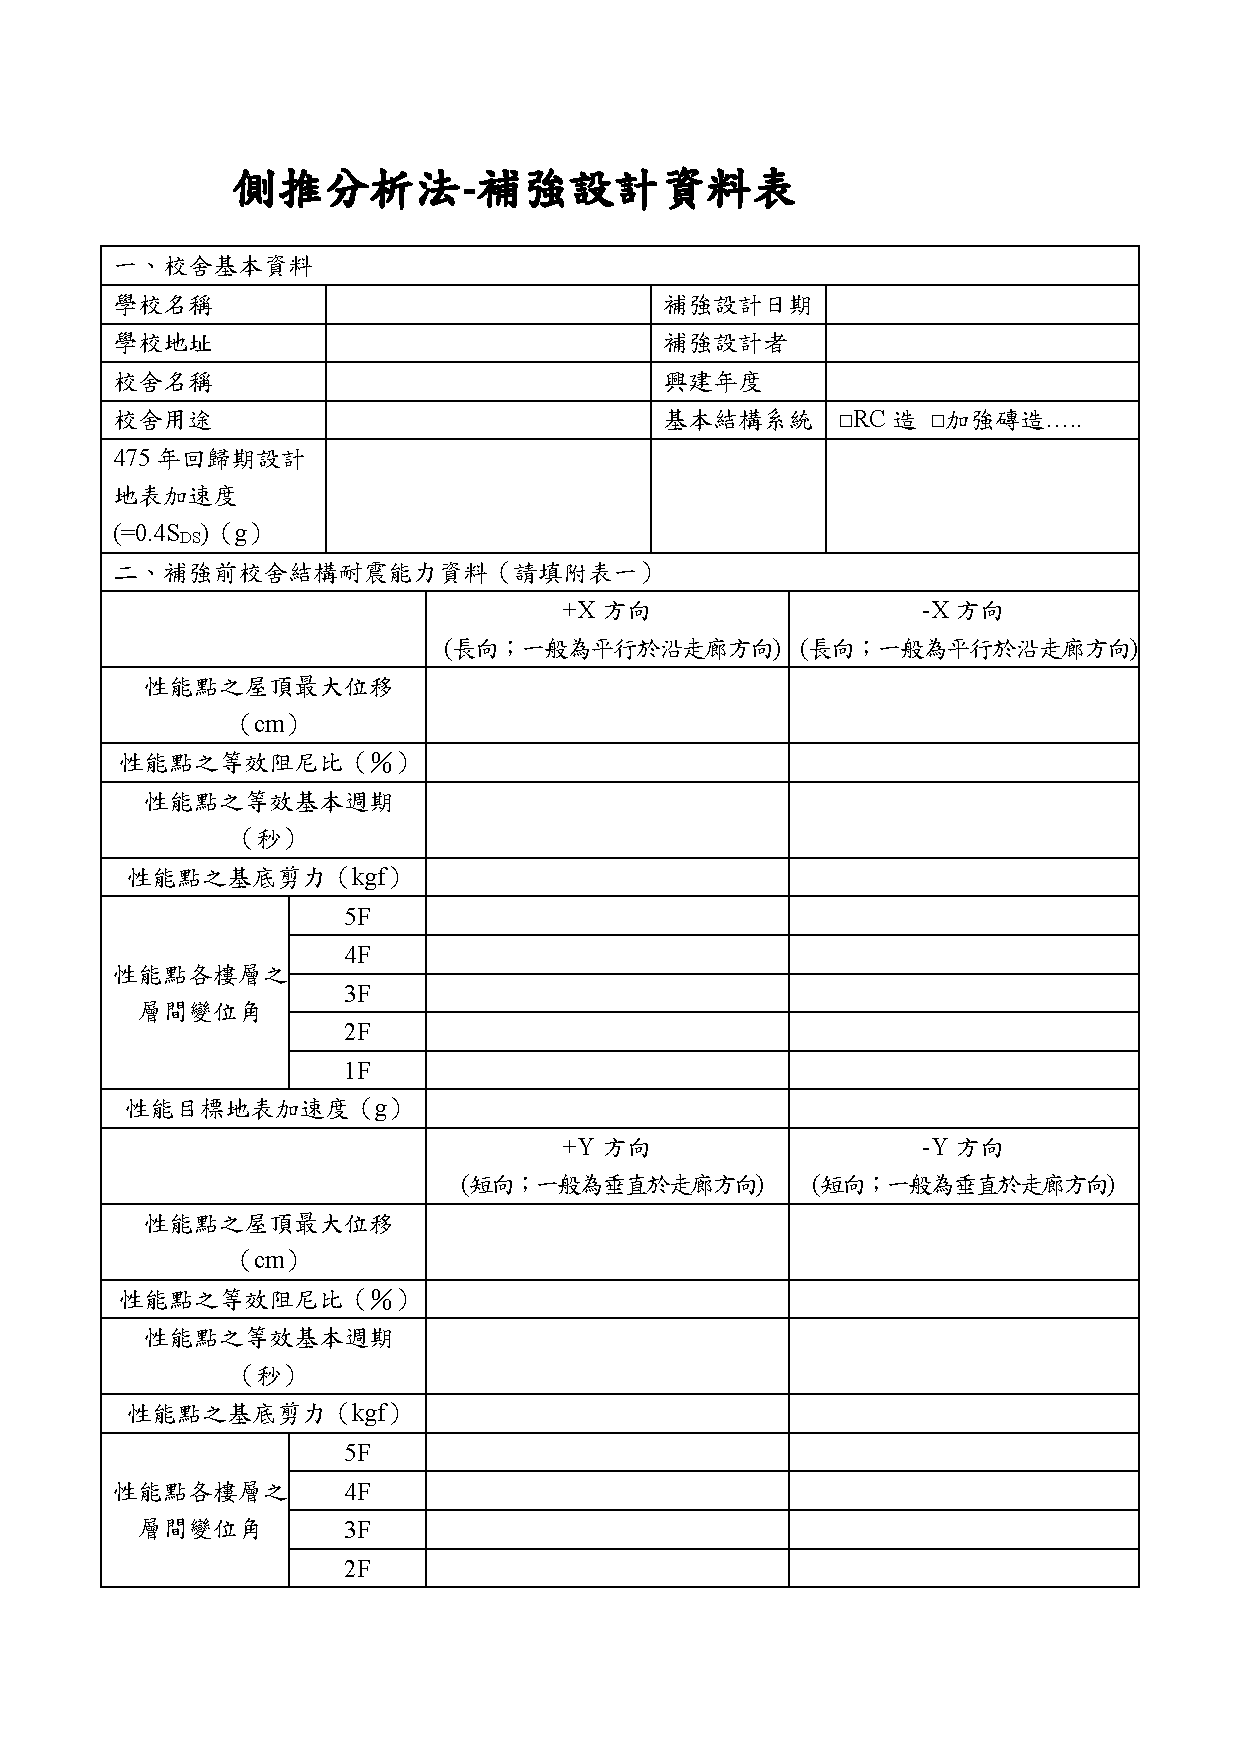
\includepdf[fitpaper=true,scale=0.95]{appendix/retrofit.pdf}

%%% 自傳
%\newpage
%\chapter*{\protect\makebox[5cm][s]{\nameVita}} % \makebox{} is fragile; need protect
%\addcontentsline{toc}{chapter}{\nameVita}
%本人生於 1981 年 1 月 1 日,在桃園內壢。家裡經營電器行,上有一位姊姊。從小就喜歡拆解店裡收回的報廢家電用品,練就了一身好手藝與探究一切的好奇心。

國小就讀平鎮國小。由於把供應全校用水的抽水馬達拆開研究裝不回去,造成全校停水,廁所污穢不堪。被校長處罰掃廁所一個星期。那真是我少時年幼無知的一頁插曲。



%%%%%%%%%%%%%%%%%%%%%%%%%%%%%%%
%       授權書 (計頁碼,但不印頁碼) 
%%%%%%%%%%%%%%%%%%%%%%%%%%%%%%%
%
% insert the printed standard form when the thesis is ready to bind
% 在口試完成後,再將已簽名的授權書放入以便裝訂
% create an entry in table of contents for 授權書
% 目前送出空白頁
\cleardoublepage
\phantomsection
%
\includepdf[fitpaper=true,scale=1,pagecommand=\thispagestyle{empty}]{backpages/G-15.pdf}

\includepdf[fitpaper=true,scale=1,angle=90,pagecommand=\thispagestyle{empty}]{backpages/img-122151637-0001.pdf}


	%\bibliographystyle{unsrt} 



\end{document} 
 
